% LaTeX source for 'Python: In Hydrology'
% Copyright (c)  2011  Sat Kumar Tomer

% Permission is granted to copy, distribute and/or modify this
% document under the terms of the GNU Free Documentation License,
% Version 1.1  or any later version published by the Free Software
% Foundation; with no Invariant Sections, no Front-Cover Texts,
% and no Back-Cover Texts.

% This distribution includes a file named fdl.tex that contains the text
% of the GNU Free Documentation License.  If it is missing, you can obtain
% it from www.gnu.org or by writing to the Free Software Foundation,
% Inc., 59 Temple Place - Suite 330, Boston, MA 02111-1307, USA.
%

% ACKNOWLEDGEMENT
% I am using the Latex file of Allen Downey
% which he used in the book, 'Think Python: How to Think Like a Computer Scientist'.

\documentclass[10pt]{book}
\usepackage[width=5.5in,height=8.5in,
  hmarginratio=3:2,vmarginratio=1:1]{geometry}

% for some of these packages, you might have to install
% texlive-latex-extra (in Ubuntu)

\usepackage[utf8]{inputenc}
\usepackage{pslatex}
%\usepackage{url}
\usepackage{fancyhdr}
\usepackage{graphicx}
\usepackage{amsmath, amsthm, amssymb} 
\usepackage[pdfborder={0 0 0}]{hyperref} 
\usepackage{exercise}                        % texlive-latex-extra
\usepackage{makeidx}
\usepackage{setspace}
\usepackage{hevea}                           
\usepackage{upquote}
\usepackage{listings}
\usepackage{booktabs}
\usepackage{tikz}
\usepackage{wallpaper}
\usetikzlibrary{shapes,arrows}
\definecolor{myred}{cmyk}{0.1,1.0,0.6,0.2}
\definecolor{myblue}{cmyk}{1.0,0.5,0.0,0.60}

\hypersetup{
  colorlinks = true,
  urlcolor = myblue,
  linkcolor = myblue,
  pdfauthor = {sat kumar},
  pdfkeywords = {python, hydrology},
  pdftitle = {Python in Hydrology by S. K. Tomer},
  pdfpagemode = UseNone
}

\makeindex

\title{Python}
\newcommand{\thetitle}{Python: In Hydrology}
\newcommand{\theversion}{0.1.0}

% these styles get translated in CSS for the HTML version
\newstyle{a:link}{color:black;}
\newstyle{p+p}{margin-top:1em;margin-bottom:1em}
\newstyle{img}{border:0px}

% change the arrows
\setlinkstext
  {\imgsrc[ALT="Previous"]{back.png}}
  {\imgsrc[ALT="Up"]{up.png}}
  {\imgsrc[ALT="Next"]{next.png}}

\makeindex

\begin{document}
\ThisTileWallPaper{8.5in}{11in}{images/cover.png}

\frontmatter

% LATEXONLY

\input{latexonly}

\newtheorem{ex}{Exercise}[chapter]

\begin{latexonly}

\renewcommand{\blankpage}{\thispagestyle{empty} \quad \newpage}

%\blankpage
%\blankpage

% TITLE PAGES FOR LATEX VERSION

%-half title--------------------------------------------------
\thispagestyle{empty}

\begin{flushright}
\vspace*{2.0in}

%\begin{spacing}{3}
%{\Huge Python}\\
%{\Large In Hydrology}
%\end{spacing}

\vspace{0.25in}

%Version \theversion

\vfill

\end{flushright}

%--verso------------------------------------------------------

\blankpage
%\clearemptydoublepage
%\pagebreak
%\thispagestyle{empty}
%\vspace*{6in}

%--title page--------------------------------------------------
\pagebreak
\thispagestyle{empty}

\begin{flushright}
\vspace*{2.0in}

\begin{spacing}{3}
{\Huge Python}\\
{\large In Hydrology}
\end{spacing}

\vspace{0.25in}

Version \theversion

\vspace{1in}


{\huge Sat Kumar Tomer } \vspace{0.15in} \\ 



\vspace{0.5in}

\vfill
%{\Large Green Tea Press}

%{\small Needham, Massachusetts}

%\includegraphics[width=1in]{images/logo1.eps}


\end{flushright}


%--copyright--------------------------------------------------
\pagebreak
\thispagestyle{empty}

{\small
Copyright \copyright ~2011 Sat Kumar Tomer.


Printing history:

\begin{description}

\item[November 2011:] First edition of {\em Python in Hydrology}.
\item[January 2012:] Added sections on variogram analysis, Kriging, bias correction, and calling external commands from Python. 
\item[August 2012:] Fully edited the book.
\end{description}

\vspace{0.2in}

\begin{flushleft}
Green Tea Press       \\
9 Washburn Ave \\
Needham MA 02492
\end{flushleft}

Permission is granted to copy, distribute, and/or modify this document
under the terms of the GNU Free Documentation License, Version 1.1 or
any later version published by the Free Software Foundation; with no
Invariant Sections, no Front-Cover Texts, and with no Back-Cover Texts. \\

The GNU Free Documentation License is available from \url{www.gnu.org}
or by writing to the Free Software Foundation, Inc., 59 Temple Place,
Suite 330, Boston, MA 02111-1307, USA. \\ 

The book is originally in the form \LaTeX\ source code. 
A pdf (portable document format) or ps (post script) format can be obtained 
by compiling this \LaTeX\ source code. The latest \LaTeX\ source code for the 
book is available from svn repository hosted at google code 
\url{http://www.google.code/p/python-in-hydrology/}. 

\vspace{0.2in}

} % end small

\end{latexonly}


% HTMLONLY

\begin{htmlonly}

% TITLE PAGE FOR HTML VERSION

{\Large \thetitle}

{\large Sat Kumar Tomer} \\


Version \theversion

\setcounter{chapter}{-1}

\end{htmlonly}

\chapter{Preface}

\section*{History}

I started using Python in July 2010. I was looking for a programming language, 
which is open source, and is capable of combining many codes/modules/software. 
I came across Python and Perl, though there might be many more options available. 
I googled the use of Python and Perl in the field of general scientific usage, 
hydrology, Geographic Information System (GIS), and statistics etc. 
I somehow felt Python to be the language of my need. 
I do not know if my conclusions (in the areas mentioned above) about the Python 
versus Perl were true or not? But I feel happy for Python being my choice, 
and it is fulfilling my requirements completely. \\

After using Python for two-three months, I become fond of open source, 
and started using only open source software, I said good-bye to Windows, 
ArcGis, and MATLAB etc. And even after one year, I did not miss them. 
I felt that I should also make a small contribution into the free world. 
I tried to contribute in few areas, but could not go ahead because of my 
less knowledge in those areas. After spending extensive one year with Python, 
I thought to make some contribution into Python world. 
I wrote few small packages for the Python, and started writing this book. \\

I always have been scared of reading books, 
especially those having more than 200 pages. 
I do not remember if I have read any book completely, 
which had more than 200 pages. Though the list of books, 
that I have read is very small, even for the books which had pages less than 200. 
I do not like much of the text in the book, 
and like to learn from examples in the book. 
I am a student, not a professor, so does not have any idea about what students 
like except my own feeling, which I know many of my fellow students do not like. \\

I hope that you will find this book helpful and enjoyable. \\

\vfill


Sat Kumar Tomer \\
Bangalore, India\\

Sat Kumar Tomer is a Phd Student in the Department of Civil Engineering at 
Indian Institute of Science, Bangalore, India.


\section*{Acknowledgements}

I am thankful to you for reading the book, and hope to receive feedback from you.

I am thankful to Allen B. Downey who provided the latex source code of his books, 
which helped me in formatting the book in a better way. Apart from it, 
he has written a nice history for his book titled `Think Python: How to Think Like
a Computer Scientist', which encouraged me for writing this book. 
And, I \textbf{copied} many sentences from his book, mainly the basic about Python. \\

I am thankful to the Free Software Foundation for developing the 
GNU Free Documentation License. \\

I am thankful to Green Tea Press. \\

I am thankful to my friends Aditya Singh, Ganjendara Yadav, 
Himanshu Joshi, Katarina Turcekova, Shadi Davarian, and Shobhit Khatyan 
for their continuous support. \\

\section*{Suggestions/corrections}
If you have a suggestion or correction, you are more than 
welcome to drop an email at \url{satkumartomer@gmail.com}. \\


\normalsize

\clearemptydoublepage

% TABLE OF CONTENTS
\begin{latexonly}

\tableofcontents

\clearemptydoublepage

\end{latexonly}

% START THE BOOK
\mainmatter

\chapter{Getting started}

\section{Why Python?}
Python is a simple and powerful programming language. 
By simple I mean, that it is much more forgiving than languages like 
C though slow also. By powerful, I mean it can glue many existing codes,  
which were written in C, C++, Fortran etc. easily. 
It has a growing user community, which makes many tools easily available. 
Python Package Index, which is a major host of the Python code, 
has more than 15,000 packages listed as of now, speaks about it popularity. 
The use of Python in hydrology community is not so fast as compared to other field, 
but now-a-days many new hydrological packages are being developed. 
Python provides access to a nice combination of GIS tools, Mathematics, 
and Statistics etc., which makes it a useful language for the hydrologist. 
Following are the major advantages of Python for the hydrologist:
\begin{enumerate}
\item A clear and readable syntax. \
\item Modules can be easily written in C, C++. \
\item It can be used on all major platforms (Windows, Linux/Unix, Mac etc.) \
\item Easy to learn. \
\item And, it is free. \
\end{enumerate}

\index{Why Python}

\section{Python Installation}
Usually all the Linux/Unix system has basic Python installed by-default. If you are in
some other platform (Windows or Mac), or for some reason your Linux/Unix do not have 
a basic version of Python installed, you can use the below instructions to install the 
basic version of Python depending upon on your platform.  
The basic version of Python includes minimal packages required to run the python. 
Often additional packages are required to do the required tasks, specially for most 
of the hydrological applications, the basic version of python is not enough, 
and additional packages are must. The next section will describe the installation 
procedure for required additional packages. 
Throughout the book, the chevron (\verb">>>") represents the Python shell, 
and {\verb" $"} represents the Unix/Linux shell or window's command line. 
The installation of Python for the various operating system is done in the 
following ways

\index{Install Python}

\subsection{Ubuntu/Debian}
In the Ubuntu/Debian, the Python is installed by running the usual installation command, i.e.:
\beforeverb
\begin{verbatim}
$ sudo apt-get install python
\end{verbatim}
\afterverb

\index{apt-get}

\subsection{Fedora}
On Fedora, the installation of the Python is performed by using the following command:
\beforeverb
\begin{verbatim}
$ sudo yum install python
\end{verbatim}
\afterverb

\index{yum}

\subsection{FreeBSD}
Python is installed on FreeBSD by running:
\beforeverb
\begin{verbatim}
$ sudo pkg_add install python
\end{verbatim}
\afterverb
\index{pkg_add}

The Linux user might be familiar with \verb"sudo". 
It allows user to run programs with the security privileges of root or administrator. 
Window user may ignore \verb"sudo", as they do not need to specify this. \\

\subsection{Windows}
For Windows users, the suitable version of Python can be downloaded 
from \url{http://www.python.org/getit/}. 
It provides a .msi file, which can be easily installed by double clicking on it. \\

\subsection{Mac OS}
Mac OS users also can download a suitable version of Python from 
\url{http://www.python.org/getit/} and install it.

\index{Fedora}
\index{Ubuntu/Debian}
\index{FreeBSD}
\index{Windows}
\index{Mac OS}

\section{Install Additional Packages}
\label{install}
Pip is a useful program to install additional packages in Python, which provides an 
easiest way to install additional packages. 
Before installing pip, \verb"distribute" should be installed. 
To do so, first we need to download \verb"Distribute", 
which is done by downloading \verb"distribute_setup.py" file from 
\url{http://python-distribute.org/distribute\_setup.py}, 
and running the following command:
\beforeverb
\begin{verbatim}
$ sudo python distribute_setup.py
\end{verbatim}
\afterverb
Note again for Windows users the \verb"sudo" is not needed, and you can use the command
without using it. \\

\index{Install additional packages}

Now download the \verb"get-pip.py" from 
\url{https://github.com/pypa/pip/raw/master/contrib/get-pip.py}, and run as root:
\beforeverb
\begin{verbatim}
$ sudo python get-pip.py
\end{verbatim}
\afterverb

Note, that the \verb"distribute_setup.py" and \verb"get-pip.py" should be in 
your current working directory while installing, otherwise give the full path 
name of file. If you did not get any error in this procedure, \verb"pip" should 
be ready to install new packages. The procedure to install packages is simple, let's say
we want to install package \verb"SomePackage", then we need to run the following command:
\beforeverb
\begin{verbatim}
$ sudo pip install SomePackage
\end{verbatim}
\afterverb

In hydrology, frequently used packages are \verb"Numpy", \verb"Scipy", \verb"xlrd", 
\verb"xlwt", and \verb"gdal", so we will install all of them at this stage. 
Late, whenever a new package/library will be required, instructions to download and 
install them will be given there. 
\beforeverb
\begin{verbatim}
$ sudo pip install Numpy
$ sudo pip install Scipy
$ sudo pip install xlrd
$ sudo pip install xlwt
$ sudo pip install gdal
\end{verbatim}
\afterverb
These packages/libraries can be installed by specifying all packages name in one line, 
i.e. \verb"$ sudo pip install Numpy Scipy xlrd xlwt gdal". 
But, at this time it is better to install them in separate line, 
so that if you get some error, you can easily find out which package is giving error.  
The most common problem with \verb"pip" is that, it is not able to download 
library/package from internet. It happens mainly when you use some proxy to connect
to the internet. In that case, we can download the \verb"*.tar.gz" file of the library 
using internet browser, and then run the \verb"pip" in the following way:
\beforeverb
\begin{verbatim}
$ sudo pip install /path/to/*.tar.gz
\end{verbatim}
\afterverb
Windows user can download \verb"*.exe" or \verb"*.msi" file if available and then 
install by double clicking it. \\

If this also fails then, as a last option, you can download \verb"*.tar.gz" file 
and extract it. Then, go to the folder where you have extracted the file. 
There, you should see the \verb"setup.py" file. Now, run the following command:
\beforeverb
\begin{verbatim}
$ sudo python setup.py install 
\end{verbatim}
\afterverb
If you see any error in this, which could possibly arise because of non-availability
of some dependent package/library in your computer. 
You should read the \verb"README" file provided with the package, 
it can provide you details of required package/library, and how to install them. \\

The package/libraries are upgraded using the pip in the following way.
\beforeverb
\begin{verbatim}
$ sudo pip install --upgrade some_package
\end{verbatim}
\afterverb
\index{Upgrade packages}

\section{Interactive Development Environment}
Simple text editors can be used to write Python programs, but these do not provide 
options for easy formatting of text, auto completion of text, and debugging options etc.  
IDE (Interactive Development Environment) provides many options to quickly format 
the program in Python way, and easily debug them. There are various IDE available 
for use e.g. PyDev, Spyder, IDLE, and many many others. A list of them can be 
found at \url{http://wiki.python.org/moin/IntegratedDevelopmentEnvironments}. 
I am using Spyder for my work, which is similar to MATLAB. The reason to use 
Spyder was since earlier I used to work on MATLAB, and Spyder is similar to it, 
so I found myself to be familiar with it. However, you can use any IDE, and after 
being familiar, it doesn't matter which one you use. 
\index{IDE}

\section{Execute the Program}
Python is an interpreted language as the programs are executed by an interpreter. 
There are two ways to use the interpreter: 
{\bf interactive mode} and {\bf script mode}. 
In the interactive mode, you type Python programs (after invoking the python, 
which is done by typing {\verb"python" in a terminal or command window) and 
interpreter prints the result, e.g. we do \verb"1+1" in it.
\index{Execute}

\beforeverb
\begin{verbatim}
$ python
>>> 1 + 1
2
\end{verbatim}
\afterverb
When you invoked Python, you will also see other details like version of Python. \\ 

The chevron, \verb">>>", is the {\bf prompt} which interpreter uses to indicate 
that it is ready. If you type {\tt 1 + 1}, the interpreter replies {\tt 2}. 
Alternatively, you can store code in a file and use the interpreter to execute 
the contents of the file, which is called a {\bf script}.  By convention, Python 
scripts have names that end with {\tt .py}. Suppose, you have named you script as 
{\tt myscript.py}, and you want to execute it, in a Unix/Linux shell, you would do:
\beforeverb
\begin{verbatim}
$ python myscript.py
\end{verbatim}
\afterverb
or, you can give your script executable permission and simply run the script. 
The syntax to do is:
\beforeverb
\begin{verbatim}
$ chmod +x myscript.py
$ ./myscript.py
\end{verbatim}
\afterverb

In KDE's, the details of executing scripts are different.  
You can find instructions for your environment at the Python website \url{python.org}. \\


Working in interactive mode is convenient for testing small pieces of code because 
you can type and execute them immediately.  But for anything more than a few lines, 
you should save your code as a script so you can modify and execute it in the future. \\


\section{Type of Errors}
Three kinds of errors can occur in a program: syntax errors, runtime  errors, and 
semantic errors. It is useful to distinguish between them in order to track them down 
more quickly. \\
\index{Type of errors}

\subsection{Syntax Errors}
Python can only execute a program if the syntax is correct; otherwise, the interpreter 
displays an error message. {\bf Syntax} refers to the structure of a program and the 
rules about that structure. For example, parentheses have to come in matching pairs, 
so \verb" (1 + 2) " is legal, but \verb" 8) " is a {\bf syntax error}. \\ 
\index{Type of errors! Syntax Errors}

\subsection{Runtime Errors}
The second type of error is a runtime error, so called because the error does not appear 
until after the program has started running. These errors are also called {\bf exceptions} 
because they usually indicate that something exceptional (and bad) has happened. \\
\index{Type of errors! Runtime Errors}

\subsection{Semantic Errors}
The third type of error is the {\bf semantic error}.  If there is a semantic error in your 
program, it will run successfully in the sense that the computer will not generate any 
error messages, but it will not do the right thing. \\
\index{Type of errors! Semantic Errors}

\section{The First Program}
Traditionally, the first program you start with in a new language is ``Hello, World!'' program,
because all it does is display the words, ``Hello, World!''. In Python, it is done by following
syntax of codes:

\beforeverb
\begin{verbatim}
>>> print 'Hello, World!'
\end{verbatim}
\afterverb
This is an example of a \verb"print" statement, which prints on computer screen. 
In this case, the result is the sentence:
\beforeverb
\begin{verbatim}
Hello, World!
\end{verbatim}
\afterverb
The quotation marks in the program mark the beginning and end of the string. \\
\index{Hello, World program}


\chapter{A Bit of Python}
Before jumping into applications of Python programming language into hydrology, 
which would involve writing many lines of codes, it is better to first learn some basics 
of Python, e.g. the types of data, looping (performing same task many times), 
and writing functions etc. Let's begin with the types of data that we are going to deal
with. Note that there are few more data types, and you may create your own data type,
we will not touch on these issues, as they involve more in-depth knowledge of Python. \\ 

\section{Data Types}
There are basically two types of data in Python: numbers and strings. 
The \verb"type" function can be used to check the type of data. \\
\index{Data type}

\subsection{Numbers}
There are three types of number in Python: integers, floating point and complex numbers. 
Integers are needed for indexing the arrays (vector, matrix), and counting etc. 
In Python there is no need to define the variable types a priori, and you are even allowed to 
change the data type later in the program, wherever needed. 
\beforeverb \begin{verbatim}
>>> a = 5
>>> type(a)
<type 'int'>
\end{verbatim} \afterverb

This means that, the data type of variable \verb``a'' is integer. 
The lines in the program without chevron (\verb">>>") represents the output by the Python. 
Another most commonly used data type is float. Most of the hydrological variables belongs to 
this category of data type. 
\beforeverb
\begin{verbatim}
>>> b = 7.8
>>> type(b)
<type 'float'>
\end{verbatim}
\afterverb
This tells that the data type is floating point. Another data type is complex, which is not 
frequently needed in day to day hydrological life. 
\beforeverb
\begin{verbatim}
>>> c = 5 + 2j
>>> type(c)
<type 'complex'>
\end{verbatim}
\afterverb
The variable \verb"c" represents the complex data type.
\index{Data Types! Integers}
\index{Data Types! Float}
\index{Data Types! Complex}

\subsection{Strings}
A string is a sequence of characters. There are mainly three following way to specify a string.
\index{Data Types! Strings}

\subsubsection{Single Quotes}
The text written inside single quotes is treated as string by Python. 
\beforeverb
\begin{verbatim}
>>> foo = 'my name is Joe'
>>> print(foo)
my name is Joe
\end{verbatim}
\afterverb

\subsubsection{Double Quotes}
Double quotes are also used to define a string. One may ask the question, ``If single quotes 
are able to define a string, then why are double quotes needed?'' Let's try to write 
\verb" What's your name? " using single quotes.
\beforeverb
\begin{verbatim}
>>> foo = 'what's your name?'
File "<stdin>", line 1
    foo = 'what's your name?'
                ^
SyntaxError: invalid syntax
\end{verbatim}
\afterverb
This produces \verb"SyntaxError". Because Python did not find pairs of single quotes, and hence 
Python could not decide which two single quotes to consider for identifying the string. Now,
let's try defining the same string using double quotes. 

\beforeverb
\begin{verbatim}
>>> foo = "what's your name?"
>>> print(foo)
what's your name?
\end{verbatim}
\afterverb
As you might have noticed that double quotes provide an easy way to define strings,
which involve single quotes. The same task can be performed using single quote also, by
telling Python which of the single quote should not be used to identify the beginning
and ending of the string. The \verb"\" is used before null single quote. Lets write the same 
string using single quotes only by using the  before \verb" ' ". 
\beforeverb \begin{verbatim}
>>> foo = 'what\'s your name?'
>>> print(foo)
what's your name?
\end{verbatim} \afterverb

\subsubsection{Triple Quotes}
When the strings spans over more than one line, triples quotes are best to define them. 
Multi-line strings can also be specified using escape sequence \verb"\n" in single or 
double quote strings, however triple quotes make it easier to write. 
Triple quotes are also useful for other things (making help content for functions) also, 
which you will read later in the book.
\beforeverb
\begin{verbatim}
>>> foo = """My name is Sat Kumar.
... I am in PhD """
>>> print foo
My name is Sat Kumar.
I am in PhD 
\end{verbatim}
\afterverb


\section{Data structures}
Data structures are able to contain more than one data in it. 
There are four built-in data structures in Python: 
\verb"list", \verb"tuple", \verb"dictionary" and \verb"set". 
Apart from these built-in data structure, you can define your own data type also 
like \verb"numpy.array" defined by \verb"numpy", which is very useful. 
I did not feel any need to use the \verb"set" in hydrology, so I am skipping \verb"set" here, 
if you are interested you can learn about it from some other sources. 
\index{Data structures}

\subsection{List}
A list is a sequence of items (values). The items in it could belong to any of data type, and could be of different data type in the same list. 
\beforeverb \begin{verbatim}
>>> a = ['Ram', 'Sita', 'Bangalore', 'Delhi']
>>> b = [25, 256, 2656, 0]
>>> c = [25, 'Bangalore'] 
\end{verbatim} \afterverb
The items in the list are accessed using the indices. The variable \verb"a" and \verb"b" hold items of similar data types, while \verb"c" holds items of different data types. In Python, the indices starts at {\tt 0}. So, to get the first and third item, the indices should be 0 and 2.
\beforeverb
\begin{verbatim}
>>> a = ['Ram', 'Sita', 'Bangalore', 'Delhi']
>>> print a[0]
Ram
>>> print a[2]
Bangalore
\end{verbatim}
\afterverb

\index{Negative indices}
Negative indices are also allowed in Python. The last item in the list has \verb"-1" indices, similarly second last item has indices of \verb"-2" and so on.
\beforeverb
\begin{verbatim}
>>> a = ['Ram', 'Sita', 'Bangalore', 'Delhi']
>>> print a[-1]
Delhi
\end{verbatim}
\afterverb
Likewise, second last item in the list can be accessed by using the indices \verb"-2".

\subsection{Dictionary}
In the list, the indices are only integers. Dictionary has the capability to take any data type as indices. This feature of dictionary makes it very suitable, when the indices are name etc. For example, in hydrology the name of field stations and their corresponding variables are given for each station. Let us try to retrieve the value of variable by using list first, and then by using dictionary. We can use one list to store the name of stations, and one for the variable. First, we need to find the indices of station, and then use this indices to access the variable from the list of variables. 
\beforeverb \begin{verbatim}
>>> names = ['Delhi', 'Bangalore', 'Kolkata']
>>> rainfall = [0, 5, 10]
>>> print(rainfall[1])
5
\end{verbatim} \afterverb

Now, let us try this using dictionary. 
\beforeverb \begin{verbatim}
>>> rainfall = {'Delhi':0, 'Bangalore':5, 'Kolkata':10}
>>> rainfall['Bangalore']
5
\end{verbatim} \afterverb
The same thing could have been done using list in one line, but dictionary provides a neat and clean way to do this. 

\subsection{Tuple}
A \verb"tuple" is a sequence of values, similar to the list except that \verb"tuples" are immutable (their value can not be modified).
\beforeverb \begin{verbatim}
>>> foo = 5,15,18
>>> foo[2]
5
>>> foo[1] = 10
Traceback (most recent call last):
  File "<stdin>", line 1, in <module>
TypeError: 'tuple' object does not support item assignment
\end{verbatim} \afterverb
While trying to modify the items in the \verb"tuple", Python issues an error. Tuples are useful, when there is a need to specify some constants, and to make sure that these constants do not change. The immutable property of \verb"tuples" ensures that during executions of the program the value of constants would not change. 

A \verb"tuple" having only one item is defined by using the \verb" ',' " after this, e.g. :
\beforeverb \begin{verbatim}
>>> foo = 5
>>> type(foo)
<type 'int'>
>>> foo = 5,
>>> type(foo)
<type 'tuple'>
\end{verbatim} \afterverb
You might have noticed that without using the comma ('), Python does not treat the variable as \verb"tuple". 

\subsection{Numpy.array}
NumericalPython (NumPy) is a library/package written mainly in C programming language, but application programming interface (API) is provided for Python. The library provides \verb"numpy.array" data type, which is very useful in performing mathematical operations on the arrays. It is the type of data, that we would be dealing most of the time. This library is not a part of the standard Python distribution, hence before using this, \verb"NumPy" have to be installed in the system. We can check if \verb"NumPy" is installed in our system or not, by using the following command:
\beforeverb \begin{verbatim}
$ python -c'import numpy'
\end{verbatim} \afterverb

If this command gives no output (no error), then it means that \verb"NumPy" is installed. If \verb"NumPy" is not installed in the system, you will see some message (error) like following:
\beforeverb
\begin{verbatim}
$ python -c'import numpy'
Traceback (most recent call last):
  File "<string>", line 1, in <module>
ImportError: No module named numpy
\end{verbatim} \afterverb

This means, that \verb"numpy" is not installed in the system. You can install \verb"NumPy" by following the steps provided in the section \ref{install}. The \verb"python -c'import numpy'" is a way to run some simple code without invoking the python. This is useful when you want to do something small, quickly. This is very helpful when you want to check if some package is installed or not in your system. \\

Before using any library, it should be imported into the program. The \verb"import" can be used to import the library. There are three ways to import a complete library or some functions from the library. By importing complete library:
\beforeverb \begin{verbatim}
>>> import numpy
>>> x = [1, 2, 5, 9.0, 15]  # list containing only numbers (float or integers)
>>> type(x)
<type 'list'>
>>> x = numpy.array(x) # convert the list into numpy array
>>> type(x)
<type 'numpy.ndarray'>
\end{verbatim} \afterverb
We imported the complete library \verb"numpy", and after doing so, whenever we need any function (i.e. \verb"array") from this library, we need to provide name along with the name of library (i.e. \verb"numpy.array"). The array function converts a list of integers or/and float into \verb"numpy array". Often the library name are quiet long, and it can be abbreviated using \verb"as" in the following manner. 
\beforeverb \begin{verbatim}
>>> import numpy as np
>>> x = np.array(x) # convert the list into numpy array
>>> type(x)
<type 'numpy.ndarray'>
\end{verbatim} \afterverb

If only few functions are needed then they can be imported by explicitly defining their name:
\beforeverb \begin{verbatim}
>>> from numpy import array
>>> x = array(x) # convert the list into numpy array
>>> type(x) 
<type 'numpy.ndarray'>
\end{verbatim} \afterverb

If all the functions are needed, and you do not want to use \verb"numpy" or \verb"np" before them, then you can import in the following way.
\beforeverb \begin{verbatim}
>>> from numpy import *
>>> x = array(x) # convert the list into numpy array
>>> type(x) 
<type 'numpy.ndarray'>
\end{verbatim} \afterverb

Anything written after \verb"#" is comment for program, and Python does not execute them. Comments are useful in making your code more readable. The comments can be in full line also. A \verb"numpy array" is a homogeneous multidimensional array. It can hold only integer, only float, combination of integers and float, complex numbers and strings. If combination of integers and float are specified in \verb"numpy.ndarray", then integers are treated as floats. The data type of \verb"numpy.ndarray" can be checked using its attribute \verb"dtype". 
\beforeverb \begin{verbatim}
>>> import numpy as np
>>> x = np.array([1,5,9.0,15]) # np.array can be defined directly also
>>> x.dtype
dtype('float64')
>>> x = np.array([1,5,9,15]) # this is holding only integers
>>> x.dtype
dtype('int64')
>>> x = np.array(['Delhi', 'Paris']) # this is holding strings
>>> x.dtype
dtype('|S5')
\end{verbatim} \afterverb
The mean of the array can be computed using method \verb"mean", in the following manner.
\beforeverb
\begin{verbatim}
>>> import numpy as np
>>> x = np.array([1,5,9.0,15]) 
>>> x.sum()
30.0
\end{verbatim}
\afterverb
Did you notice the difference between calling attributes and methods? The methods perform some action on the object, and often action needs some input, so methods are called with brackets \verb"()". If there is some input to be given to method, it can be given inside brackets, if there is no input then empty brackets are used. Try using the methods (e.g. sum) without giving the bracket, you will see only some details about it, and no output. 
\index{Attribute}
\index{Method}

As Python is object oriented programming (OOP) language, and attributes and methods are used quiet commonly. It is better to know briefly about them before jumping into Python. \verb"Attributes" represent properties of an object, and can be of any type, even the type of the object that contains it. \verb"methods" represent what an object can do. An attribute can only have a value or a state, while a method can do something or perform an action. 
\index{OOP}

\section{Choosing the name of variable}
Then name of the variables should be meaningful, and possibly should be documented what the variable is used for. 

Variable names can be arbitrarily long.  They can contain both letters and numbers, but they have to begin with a letter.
It is legal to use uppercase letters, but it is a good idea to begin variable names with a lowercase letter, as conventionally uppercase letters are used to denote classes. 

The underscore character (\verb"_") can appear in a name. It is often used in names with multiple words, such as
\verb"my_name" or \verb"airspeed_of_unladen_swallow". A variable name can be started with underscore, but should be avoided because this is used for something else conventionally. 

Python has some of the reserved keywords, which can not be used as variable name. If the interpreter gives some error about one of your variable names and you don't know why, you should check if your variable name is not in the reserved keyword list. It is a good idea to remember the list, or keep it handy. But I, being a lazy person, do not remember this list, and in fact even never tried to remember. I just type the name of variable, I want to use in python, and look for the output by python, and then decide whether to use this name for variable or not.

\beforeverb
\begin{verbatim}
>>> 500_mangoes 
  File "<stdin>", line 1
    500_mangoes 
              ^
SyntaxError: invalid syntax
>>> class
  File "<stdin>", line 1
    class
        ^
SyntaxError: invalid syntax
>>> np
<module 'numpy' from '/usr/lib/pymodules/python2.7/numpy/__init__.pyc'>
>>> foo
Traceback (most recent call last):
  File "<stdin>", line 1, in <module>
NameError: name 'foo' is not defined
\end{verbatim}
\afterverb
First variable name \verb"500_mangoes" gives \verb"SyntaxError", so we cant use this name as variable. The \verb"class" gives the \verb"SyntaxError" too, so it also can not be used. The \verb"np" gives some output (which means \verb"np" is referring to something), so if we use this as variable name, the reference will be destroyed. The \verb"foo" gives \verb"NameError" that the variable is not defined, this makes it a valid choice for the variable name. Apart from these scenarios, one more output is possible. 
\beforeverb
\begin{verbatim}
>>> a = 5
>>> a
5
\end{verbatim}
\afterverb
This means that variable \verb"a" is defined before, now it is upto you, if you want to change its old value.

\section{Operators and operands}
{\bf Operators} are special symbols that represent computations like addition and multiplication.  The values the operator is applied to are called {\bf operands}. Assume variable $a$ holds 2 and variable $b$ holds 5.

\begin{tabular}{lll}
\toprule
Operator & Name & Example \\
\midrule
+ & Plus & \verb">>> a+b" \\
  &      & 7 \\
- & Minus & \verb">>> a-b" \\
  &      & -3 \\
* & Multiply & \verb">>> a*b" \\
  &      & 10 \\
/ & Divide & \verb">>> a/b" \\
  &      & 0 (for Python 2.x) \\
  &      & 0.4 (for Python 3.x) \\
** & Power & \verb">>> a**b" \\
  &      & 32 \\
\% & Modulo & \verb">>> b\%a" \\
  &      & 1 \\
== & Equal to & \verb">>> a==b" \\
  &      & False \\
$<$ & Less than & \verb">>>a<b" \\
  &      & True \\
$>$ & Greater than & \verb">>>a>b" \\
  &      & False \\
\verb"<=" & Less than or Equal to & \verb">>>a<=b" \\
  &      & True \\
\verb">=" & Greater than or Equal to& \verb">>>a>=b" \\
  &      & False \\
\verb"!=" & Not equal to & \verb">>>a!=b" \\
  &      & True \\
and & And & \verb">>>" True and False \\
  &      & False \\
or & Or & \verb">>>" True or False \\
  &      & True \\
not & Not & \verb">>>" not True \\
  &      & False \\
$+=$ & Add AND assignment & \verb">>> a += b" \\
  &      & 7 \\
$-=$ & Subtract AND assignment & \verb">>> a -= b" \\
  &      & 3 \\
 $*=$ & Multiply AND assignment & \verb">>> a *= b" \\
  &      & 10 \\
 $/=$ & Divide AND assignment & \verb">>> a /= b" \\
  &      & 0 \\
 $\%=$ & Modulus AND assignment & \verb">>> a %= b" \\
  &      & 2 \\
 $**=$ & Exponent AND assignment & \verb">>> a **= b" \\
  &      & 32 \\
 $//=$ & Floor division AND assignment & \verb">>> a //= b" \\
  &      & 0 \\
  \bottomrule
\end{tabular}


\section{Expressions}
An {\bf expression} is a combination of values, variables, and operators. A value all by itself is considered an expression, and so is a variable, so the following are all legal expressions (assuming that the variable \verb"x" has been assigned a value:

\beforeverb
\begin{verbatim}
>>> x = 17
>>> x + 15
32
\end{verbatim}
\afterverb

If you type an expression in interactive mode, the interpreter {\bf evaluates} it and displays the result:

\beforeverb
\begin{verbatim}
>>> 1 + 1
2
\end{verbatim}
\afterverb
%
But in a script, an expression all by itself doesn't do anything!  This is a common source of confusion for beginners.


\section{Control Flow}
If we want to do same task many times, restrict the execution of task only when some condition is met, {\bf control flow} is the way to do it. 

\subsection{for}
\verb"for" is used to repeatedly execute some code. It also can be used to iterate over some list. Suppose you have some list, and you want to square the each item in list and print.
\beforeverb
\begin{verbatim}
>>> foo = [5, 11, 14, 0, 6, 0, 8] # define the list
>>> for item in foo:
...     print item**2
... 
25
121
196
0
36
0
64
\end{verbatim}
\afterverb
\index{loop, for}

The item in the list can be iterated by defining another list having integers, and iterating over it. Let us try this way to perform the above task. 
\beforeverb
\begin{verbatim}
>>> foo = [5, 11, 14, 0, 6, 0, 8] # define the list
>>> a = range(7) # define the list having integers
>>> a
[0, 1, 2, 3, 4, 5, 6]
>>> for item in a:
...     print foo[item]**2
... 
25
121
196
0
36
0
64
\end{verbatim}
\afterverb

\subsection{while}
\verb"while" statement is used, when we want to keep on executing the some code unless some condition is met or violated. Suppose, we want to print some numbers ranging from 15 to 20, we could do like this.
\beforeverb
\begin{verbatim}
>>> n = 15 # initialize the n
>>> while n<=20:
...     print n
...     n = n+1
... 
15
16
17
18
19
20
\end{verbatim}
\afterverb
\index{Statement, while}

\subsection{if}
\verb"if" statement execute some portion of the code, if the conditions are met, otherwise it skips that portion. Suppose you have some list, and you want to compute its inverse, but want to skip if the entry in list is zero:
\beforeverb
\begin{verbatim}
>>> foo = [5, 11, 14, 0, 6, 0, 8] # define the array
>>> for item in foo:
...     if item is not 0:
...         print 1.0/item
... 
0.2
0.0909090909091
0.0714285714286
0.166666666667
0.125
\end{verbatim}
\afterverb
\index{Statement, if}

The \verb"if-else" allows alternative portions of code to execute depending upon the condition. In \verb"if-else" only one portion of code is executed from the given alternatives. Suppose in the previous example, you want to issue some statement when there is 0 in the list.
\beforeverb
\begin{verbatim}
>>> foo = [5, 11, 14, 0, 6, 0, 8] # define the array
>>> for item in foo:
...     if item is not 0:
...         print 1.0/item
...     else:
...         print '0 found in list'
... 
0.2
0.0909090909091
0.0714285714286
0 found in list
0.166666666667
0 found in list
0.125
\end{verbatim}
\afterverb

\verb"if-elif-else" is used when depending upon the condition, you want to execute some portion of code. You can specify as many conditions you want, and their corresponding code to execute. Lets take one example, suppose we have one list, and we want to print some statement if the item in list is negative, positive or 0.
\begin{verbatim}
>>> foo = [5, -11, 14, 0, -6, 0, 8] # define the array
>>> for item in foo:
...     if item < 0:
...         print 'item is negative'
...     elif item>0:
...         print 'item is positive'
...     else:
...         print 'item is 0'
... 
item is positive
item is negative
item is positive
item is 0
item is negative
item is 0
item is positive
\end{verbatim}
\afterverb

\subsection{break}
The \verb"break" statement, breaks out of the loop. Suppose you want to print all the items in the list, but you want to stop the loop if you encounter 0. 
\beforeverb
\begin{verbatim}
>>> for item in foo:
...     if item==0:
...             print('zero found in the list, stopping iterations')
...             break
...     else:
...             print(item)
... 
5
-11
14
zero found in the list, stopping iterations
\end{verbatim}
\afterverb
\index{Statement, break}

The \verb"break" statement becomes useful when you want to want if something strange happens to your program, and in that condition you want to stop the execution. 

\subsection{continue}
The \verb"continue" statement provides opportunity to jump out of the current loop (iteration) when some condition is met. Suppose you do not want to print items in the list which are negative.
\beforeverb
\begin{verbatim}
>>> foo = [5, -11, 14, 0, -6, 0, 8] # define the array
>>> for item in foo:
...     if item<0:
...         continue
...     print item
... 
5
14
0
0
8
\end{verbatim}
\afterverb
\index{Statement, continue}

\subsection{pass}
\index{Statement, pass}
The \verb"pass" statement does nothing. It can be used when a statement is required syntactically but the program requires no action. 
\beforeverb
\begin{verbatim}
>>> foo = [5, -11, 14, 0, -6, 0, 8] # define the array
>>> for item in foo:
...     pass
... 
\end{verbatim}
\afterverb
This is often used, when you are developing your code, and intent to put something later. If you leave without \verb"pass", Python will issue the error.

\section{Function}
\index{Function}
Function is a some sequence of statements that does some processing. When you define a function, you specify the name and the sequence of statements.  Later, you can call the function by name. There are many built in functions in the Python, and each library provides some functions. You can also specify your functions. When you need to do some task many times, it is better to define function to do that task, and later call the function. The thumb rule is that, whenever you feel to define one function define it.

\subsection{In-built functions}
Python has some in-built functions, some of them we have already used. 
\beforeverb
\begin{verbatim}
>>> foo = [5, -11, 14, 0, -6, 0, 8] # define the array
>>> type(foo)
<type 'list'>
>>> len(foo)
7
>>> max(foo)
14
\end{verbatim}
\afterverb
Here, \verb"type", \verb"len", \verb"max" are in-built functions, which returns the \verb"type", \verb" length" of the list, and \verb"maximum" value in the list respectively. 

\subsection{User defines functions}
If you do not find the function that you intent to use, you can define one. In fact, it is a good practice to define functions whenever they are needed, it increase the readability of the codes. A function definition specifies the name of a new function and the sequence of statements that execute when the function is called.

\index{User defined functions}

Suppose, you want to define a function which adds the 2 into the input.
\beforeverb
\begin{verbatim}
>>> def add2(temp):
...     return temp+2
... 
>>> add2(5)
7
>>> foo = np.array( [5, -11, 14, 0, -6, 0, 8]) # define the array
>>> new_foo = add2(foo)
>>> print new_foo
array([ 7, -9, 16,  2, -4,  2, 10])
\end{verbatim}
\afterverb
The \verb"return" defines the output from the function. \verb"return" is optional, some functions may not return anything.

\beforeverb
\begin{verbatim}
>>> foo = [5, -11, 14, 0, -6, 0, 8] # define the array
>>> def add2(temp):
...     print temp[-1]+2 # add 2 to only the last entry in the list
... 
>>> add2(foo)
10
>>> new_foo = add2(foo)
10
>>> new_foo
\end{verbatim}
\afterverb
This is clear from this example that functions need not to return any values. Like in this example, function only print the last entry of the list after adding 2 to it, and returns none.

\section{Plotting}
There are various library which provides plotting capabilities in Python. I liked \verb"Matplotlb" library, and it is installed in the following manner.
\beforeverb
\begin{verbatim}
$ sudo pip install matplotlib
\end{verbatim}
\afterverb

Let us make our first plot which plots $y$ versus $x$. The $x$ contains values between $0$ and $2 \pi$ with 50 intervals, and $y$ is the $\sin$ of $x$.

\beforeverb
\begin{verbatim}
>>> # import the required modules
>>> import numpy as np
>>> import matplotlib.pyplot as plt
>>> # generate x over the range from 0 to 2 pi with 50 intervals
>>> x = np.linspace(0,2*np.pi,50)
>>> y = np.sin(x) # compute the sin of x
>>> plt.plot(x,y)
>>> plt.xlabel('x')
>>> plt.ylabel('y')
>>> plt.legend(['sin(x)'])
>>> plt.show()
\end{verbatim}
\afterverb
\index{plt}
\index{np}

The \verb"plt" is the given abbreviated name, which refers to the \verb"matplotlib.pyplot" library. All the function of this library should be called by using \verb"plt." while using them. The \verb"plot" makes the continuous line plot, \verb"xlabel" puts the label for the x-axis, and \verb"ylabel" puts the label for y-axis. The \verb"legend" displays the legend on the graph. \verb"show()" displays the graph, the graph can be save by using the \verb"savefig" and can be closed by using the \verb"close()". Fig. \ref{fig:1} shows the plot of $y$ versus $x$. The function \verb"np.linspace" is used to generate vector over the range $0$ to $2 \pi$ having 50 equally spaced elements. More on generating this kind of vectors is given in the next chapter. 

\beforefig
\begin{figure}[h!]
  \centering
    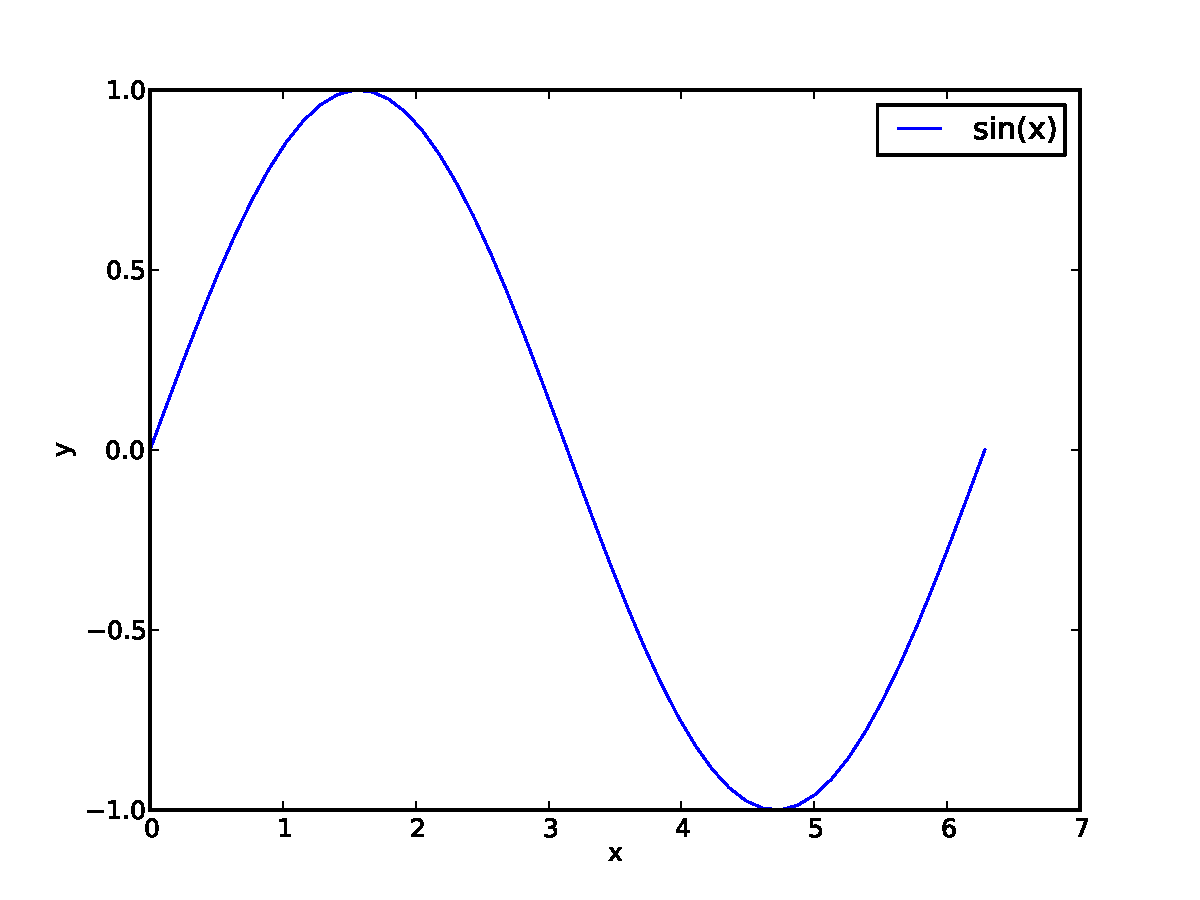
\includegraphics[width=0.5\textwidth]{images/1.pdf}
  \caption{The first plot which shows $y = \sin(x)$ versus $x$. }
  \label{fig:1}
\end{figure}
\afterfig

\chapter{Array}
\index{Array}
\section{Generating sequential arrays}
Often we need vectors whose elements follow a simple order, for example a vector containing elements \verb"[10, 11, 12, 13]" or \verb"[5, 10, 15, 20]" or \verb"[1.0, 1.2, 1.4, 1.6, 1.8, 2.0]". We see that in these vectors, items follow some simple order, so it would be nicer if there are easy way to define these kinds of vectors. Some of the way to create these vectors are following: 

\subsection{linspace}
\index{linspace}
If we are interested in generating the vector, whose elements are uniformly spaced and we know the upper, lower limit and the number of elements, then in that case \verb"linspace" is the preferred choice. 
\beforeverb
\begin{verbatim}
>>> import numpy as np
>>> np.linspace( 0, 2, 9 )       
array([ 0.  ,  0.25,  0.5 ,  0.75,  1.  ,  1.25,  1.5 ,  1.75,  2.  ])
\end{verbatim}
\afterverb
Because \verb"linspace" lies in \verb"numpy" library, so first we have imported the library and have given it an abbreviated name. Then we call the \verb"linspace" with lower limit, upper limit and the number of element to be generated. In this example, 0 is the lower limit, 2 is the upper limit, and number of elements are 9. Let us generate one more vector to understand more about this function, this time we take lower limit as 0, upper limit as $2\pi$, and number of elements to be 100.  

\beforeverb \begin{verbatim}
>>> x = np.linspace( 0, 2*pi, 100 )     
\end{verbatim} \afterverb

By default the number of elements are 50, so if we do not specify the number of elements, we get 50 elements with equal spacing. We can use \verb"len" function to get the length of any array.
\beforeverb
\begin{verbatim}
>>> foo = np.linspace(0,1)
>>> len(foo)
50
\end{verbatim}
\afterverb

\subsection{arange}
\index{arange}
Suppose again we want to generate a vector whose elements are uniformly spaced, but this time we do not know the number of elements, we just know the increment between elements. In such situation \verb"arange" is used. \verb"arange" also requires lower and upper bounds. In the following example we are generating the vector having lower element as 10, upper element as 30 and having an increment of 30. So from the knowledge of \verb"linspace" we will do something like this.
\beforeverb \begin{verbatim}
>>> np.arange( 10, 30, 5 )
array([10, 15, 20, 25])
\end{verbatim} \afterverb

Oh! What happened? Why did Python not print 30. Because \verb"arange" function does not include second argument in the elements. So we want to print upto 30, we would do.
\beforeverb \begin{verbatim}
>>> np.arange( 10, 31, 5 )
array([10, 15, 20, 25, 30])
\end{verbatim} \afterverb
This time we get the required output. The \verb"arange" can also take a float increment. Let us generate some vector with lower bound of 0, upper bound of 2 and with an increment of 0.3. 
\beforeverb \begin{verbatim}
>>> np.arange( 0, 2, 0.3 )                 # it accepts float arguments
array([ 0. ,  0.3,  0.6,  0.9,  1.2,  1.5,  1.8])
\end{verbatim} \afterverb
In the case of float increment also, the maximum value of generated elements is lesser than the second argument given to the \verb"arange".

\subsection{zeros}
\index{zeros}
\verb"zeros" is used when we want to generate all the items in vector as 0.
\beforeverb \begin{verbatim}
>>> foo = np.zeros(5)
>>> foo
array([ 0.,  0.,  0.,  0.,  0.])
\end{verbatim} \afterverb

\subsection{ones}
\index{ones}
\verb"ones" is used when all the required elements in vector are 1. Let us say, we want to generate a variable \verb"foo" which has all the elements equal to one, and has the dimension of $3 \times 2$. 

\beforeverb
\begin{verbatim}
>>> foo = np.ones((3,2))
>>> foo
array([[ 1.,  1.],
       [ 1.,  1.],
       [ 1.,  1.]])
\end{verbatim}
\afterverb
Remember that if the number of dimensions are more than one, the dimension are given as \verb"tuple", e.g. \verb"(2,5)". 

\subsection{empty}
\index{empty}
\verb"empty" is useful in initializing the variables. This assigns the garbage values to the elements, which are to be modified later. 
\beforeverb \begin{verbatim}
>>> foo = np.empty((2,5))
>>> foo
array([[  6.94573181e-310,   2.76947193e-316,   2.74957018e-316,
          0.00000000e+000,   0.00000000e+000],
       [  0.00000000e+000,   0.00000000e+000,   6.94573152e-310,
          6.34874355e-321,   0.00000000e+000]])
\end{verbatim}
\afterverb

Additionally in \verb"zeros, ones, empty", the data type (e.g. \verb"int", \verb"float" etc.) also can be defined.
\beforeverb \begin{verbatim}
>>> foo = np.empty((2,5),int)
>>> foo
array([[     140583176970856,             56931856,             59487840,
        -3617040655747907584,                    0],
       [                   0,                    0,      140583171090560,
                        1285,                    0]])
\end{verbatim} \afterverb
You can see that all the elements of \verb"foo" are now integer, even though the values are useless. 

\subsection{rand}
\index{rand}
\verb"rand" is used to generate uniformly distributed random variables over the range of 0 to 1.

\beforeverb \begin{verbatim}
>>> foo = np.random.rand(3,2)
>>> foo
array([[ 0.75644359,  0.07754619],
       [ 0.50267515,  0.91460249],
       [ 0.85992345,  0.58662329]])
\end{verbatim} \afterverb

\subsection{randn}
\index{randn}
\verb"randn" is used to generate random variable having normal distribution with mean equal to zero and variance equal to one.

\beforeverb
\begin{verbatim}
>>> foo = np.random.randn(2,4)
>>> foo
array([[-0.66317015, -1.80129451,  0.56398575, -1.11912727],
       [ 0.19218091,  0.21957804, -1.10891128, -0.87418933]])
\end{verbatim}
\afterverb

\section{Useful attributes and methods}
The \verb"ndarray" (array generated using \verb"numpy") provides attributes to perform commonly used task quickly. These attributes are used to quickly get  properties of \verb"ndarray". So let us first generate some vector whose elements are normally distributed random numbers, and try these attributes. Here I am using normally distributed random variable to demonstrate, but these attributed can be used with any \verb"numpy array". We are generating a 2 dimensional vector of size $5 \times 100$.
\beforeverb \begin{verbatim}
>>> foo = np.random.randn(5,100)
\end{verbatim} \afterverb

Let us check the number of dimension (not the size, or shape of the array). Number of dimension means how many dimensions are associated with array. For example, in mathematics terminology vector has one dimension, matrix has two dimension. 
\beforeverb \begin{verbatim}
>>> foo.ndim			
2
\end{verbatim} \afterverb
The dimension of the array is accessed by using \verb"shape" attribute.
\beforeverb \begin{verbatim}
>>> foo.shape
(5, 100)
\end{verbatim} \afterverb
The \verb"size" attribute provides the total number of elements in the array. This is simply the multiplication of all the elements given by \verb"shape" attributes. 
\beforeverb \begin{verbatim}
>>> foo.size
500
\end{verbatim} \afterverb
The data type (i.e. \verb"float", \verb"integer" etc.) is extracted using the attribute \verb"dtype".
\beforeverb \begin{verbatim}
>>> foo.dtype
dtype('float64')
\end{verbatim} \afterverb
This tells us that, the variable \verb"foo" is float, and has 64 bits. The average or mean of the variable is computed by using \verb"mean" method.
\beforeverb \begin{verbatim}
>>> foo.mean()
-0.11128938014455608
\end{verbatim} \afterverb
This provides the mean of entire array (i.e. 500 elements in this case). Suppose we want to estimate the mean across some dimension say second (1) dimension, then in this case we need to provide additional parameter to \verb"mean", i.e. \verb"axis".
\beforeverb \begin{verbatim}
>>> foo.mean(axis=1)
array([-0.07311407,  0.0705939 , -0.09218394,  0.0775191 ,  0.01026461])
\end{verbatim} \afterverb
The minimum, maximum, standard deviation and variance of the array are estimated using \verb"min", \verb"max", \verb"std", and \verb"var" methods.
\beforeverb \begin{verbatim}
>>> # to get the minimum vale
>>> foo.min()
-3.5160295160193256
>>> # to get the maximum value 
>>> foo.max()
3.0989215376354817
>>> # to get the standard deviation
>>> foo.std()
0.9528004743319175
>>> # to get the variance
>>> foo.var()
0.90782874388712709
\end{verbatim} \afterverb
Remember that the line starting with \verb"#" represents the comments. Comments make it easier to read and understand the code. So put comments whenever you do something, which is not easy to interpret from the code. \\

The trace of the matrix represent the sum of diagonal elements, and has meaning in case of square matrix. Python even allows to estimate the trace even when matrix is not square, and trace is computed by using the \verb"trace" attributes. 
\beforeverb \begin{verbatim}
>>> foo.trace()
1.081773080044246
\end{verbatim} \afterverb
There are number of attributes associated with each class, \verb"dir" function is a useful tool in exploring the attributes and method associated with any variable, class, library etc. Let us see what all methods and attributes our variable \verb"foo" have.
\beforeverb \begin{verbatim}
>>> # to get the list of all the attributes associated with foo variable
>>> dir(foo)
['T', '__abs__', ............. 'flat', 'view']
\end{verbatim} \afterverb

The output of \verb"dir(foo)" is very long, and is omitted for brevity. The attributes/method starting with \verb"_" are supposed to be the private attributes and are often not needed. 

\section{Indexing}
\index{Indexing}
In this section, we will discuss how to refer to some elements in the \verb"numpy array". Remember that in Python first indices is 0. We shall generate some array, say some array whose elements are powered to 3 of the sequence \verb"[0,1, ..., 9]".
\beforeverb \begin{verbatim}
>>> foo = np.arange(10)**3
>>> foo
array([  0,   1,   8,  27,  64, 125, 216, 343, 512, 729])
\end{verbatim} \afterverb
Print the third item in the array. Third item means we need to put indices as 2.
\beforeverb \begin{verbatim}
>>> foo[2]
8
\end{verbatim} \afterverb
Suppose, we would like to print some sequence of array, say at indices of 2,3, and 4.
\beforeverb \begin{verbatim}
>>> foo[2:5] 
array([ 8, 27, 64])     
\end{verbatim} \afterverb
We used \verb"2:5" to get the values at indices of 2,3 and 4. This is same as saying that \verb"foo[np.arange(2,5,1)]". When we do not specify the third value in the indices for array, it is by default taken as 1. If we want to print value at 2 to 8, with an interval of 3. Now because the interval is not 1, so we need to define it.
\beforeverb \begin{verbatim}
>>> foo[2:10:3]    
array([  8, 125, 512])
\end{verbatim} \afterverb
If we leave the first entry in the index as blank i.e. to get array elements form the beginning of array with an interval of 2 and upto 6, we issue the following command:
\beforeverb \begin{verbatim}
>>> foo[:6:2]    # gives the element at 0,2,4
array([ 0,  8, 64])
\end{verbatim} \afterverb
We get element upto the indices of 4, because \verb"arange" does not go upto the second argument. We can use indices also to modify the existing elements in the array, in the same way as we accessed them. Let us replace the existing value of elements at 0,2 and 4 indices, by -1000.
\beforeverb \begin{verbatim}
>>> foo[:6:2] = -1000                         # modify the elements at 0,2,4
>>> foo
array([-1000,     1, -1000,    27, -1000,   125,   216,   343,   512,   729])
\end{verbatim} \afterverb
We get the last elements of an array by indices \verb"-1". We can also use this to reverse the array, by giving the increment of -1.
\beforeverb \begin{verbatim}
>>> foo[::-1]                                 # reversed a
array([  729,   512,   343,   216,   125, -1000,    27, -1000,     1, -1000])
\end{verbatim} \afterverb
We can perform the calculation on entire \verb"numpy array" at once. Suppose we are interested in estimating the square root of the \verb"numpy array", we can use \verb"sqrt" function of \verb"numpy" library. 
\beforeverb \begin{verbatim}
>>> np.sqrt(foo) # compute the square root 
array([         nan,   1.        ,          nan,   5.19615242,
                nan,  11.18033989,  14.69693846,  18.52025918,
        22.627417  ,  27.        ])
Warning: invalid value encountered in sqrt
\end{verbatim} \afterverb

\verb"nan" represents that the element is `Not A Number'. So when the value of element is negative the output of \verb"sqrt" become \verb"nan". The Warning issued by Python tells that there were some invalid values in the input for which \verb"sqrt" can not produce any sensible output, and it provides  warning (not errors). In reality, the square root of negative number is complex number, but because we did not define the variable as complex, \verb"numpy" can not perform operations of complex numbers on this. We need library which handles complex number for such situation. 

\section{Array Manipulation}
\index{Array manipulation}
Often we need to change the array, transpose it, get some elements, or change some elements. This is illustrated by this example, in which first we create the array and then play with it. We have already seen in the previous section, that we can change the value of any element by calling it by the indices, and then assigning new value to it. First, we generate normally distributed random number of size ($2 \times 5$) to create an array, which we would like to manipulate. 
\beforeverb \begin{verbatim}
>>> foo = np.random.randn(2,3)
>>> foo
array([[ 1.02063865,  1.52885147,  0.45588211],
       [-0.82198131,  0.20995583,  0.31997462]])
\end{verbatim} \afterverb

The array is transposed using \verb"T" attributes. 
\beforeverb \begin{verbatim}
>>> foo.T
array([[ 1.02063865, -0.82198131],
       [ 1.52885147,  0.20995583],
       [ 0.45588211,  0.31997462]])
\end{verbatim} \afterverb

We can access some elements of the array, and if we want, new values also can be assigned to them. In this example, we shall first access element at (0,1) indices, and then we shall replace it by 5. Finally we will print the variable to check if the variable got modified.
\beforeverb \begin{verbatim}
>>> foo[0,1]
-0.82198131397870833
>>> foo[0,1]=5
>>> foo
array([[ 1.02063865,  5.        ],
       [ 1.52885147,  0.20995583],
       [ 0.45588211,  0.31997462]])
\end{verbatim} \afterverb

The shape of any array is changed by using the \verb"reshape" method. During reshape operation, the change in number of elements is not allowed. In the following example, first we shall create an array having size of ($3 \times 6$), and the we shall change its shape to ($2 \times 9$). 
\beforeverb \begin{verbatim}
>>> foo = np.random.randn(3,6)
array([[ 2.01139326,  1.33267072,  1.2947112 ,  0.07492725,  0.49765694,
         0.01757505],
       [ 0.42309629,  0.95921276,  0.55840131, -1.22253606, -0.91811118,
         0.59646987],
       [ 0.19714104, -1.59446001,  1.43990671, -0.98266887, -0.42292461,
        -1.2378431 ]])
>>> foo.reshape(2,9)
array([[ 2.01139326,  1.33267072,  1.2947112 ,  0.07492725,  0.49765694,
         0.01757505,  0.42309629,  0.95921276,  0.55840131],
       [-1.22253606, -0.91811118,  0.59646987,  0.19714104, -1.59446001,
         1.43990671, -0.98266887, -0.42292461, -1.2378431 ]])
\end{verbatim}
\afterverb

\index{shape}
Like we can access the any elements of the array and change it, in similar way we can access the any attributes, and modify them. However, the modification is only allowed if the attributes is writeable, and the new value makes some sense to the variable. We can use this behaviour, and change the shape of variable using the \verb"shape" attributes. 
\beforeverb \begin{verbatim}
>>> foo = np.random.randn(4,3)
>>> foo.shape
(4, 3)
>>> foo
array([[-1.47446507, -0.46316836,  0.44047531],
       [-0.21275495, -1.16089705, -1.14349478],
       [-0.83299338,  0.20336677,  0.13460515],
       [-1.73323076, -0.66500491,  1.13514327]])
>>> foo.shape = 2,6
>>> foo.shape
(2, 6)
>>> foo
array([[-1.47446507, -0.46316836,  0.44047531, -0.21275495, -1.16089705,
        -1.14349478],
       [-0.83299338,  0.20336677,  0.13460515, -1.73323076, -0.66500491,
         1.13514327]])
\end{verbatim} \afterverb

In the above example, first an array is defined with a size of ($ 4 \times 3$) and then its shape is assigned a value of (2,6), which makes the array of size ($2 \times 6$). As we can not change the number of elements, so if we define one dimension of the new variable, second dimension can be computed  with ease. Numpy allow us to define \verb"-1" for the default dimension in this case. We can make the desired change in the shape of variable by using default dimension also.
\beforeverb \begin{verbatim}
>>> foo.shape = -1,6
>>> foo.shape
(2, 6)
\end{verbatim} \afterverb
\index{ravel}

We can flatten the array (make array one dimensional) by using the \verb"ravel" method, which is explained in the following example:
\beforeverb
\begin{verbatim}
>>> foo = np.random.rand(2,3)
>>> foo
array([[ 0.82866532,  0.99558838,  0.58213507],
       [ 0.48877906,  0.67700479,  0.35975352]])
>>> foo.shape
(2, 3)
>>> a = foo.ravel()
>>> a.shape
(6,)
>>> a
array([ 0.82866532,  0.99558838,  0.58213507,  0.48877906,  0.67700479,
        0.35975352])
\end{verbatim}
\afterverb


\chapter{Basic applications in Hydrology}
\section{Introduction}
This chapter will provide applications of python in hydrology. Most of the problems given in this chapter are taken from the book titled ``Applied Hydrology" by Chow et al, and for detailed description of them, you should refer to the book. These examples include the equations commonly encountered in the hydrology. I have choose these problems to teach Python by using examples, and additionally in every example we will be learning new things about Python. \\

\section{Water Vapour}
Approximately, the saturation vapour pressure $(e_s)$ is related to the air temperature $(T)$ by the following equation,
\begin{equation}
e_s = 611 \exp\left( \frac{17.27T}{237.3+T} \right),
\end{equation}
where, $e_s$ is in pascals and $T$ is in degrees Celcius. Let us calculate the value of $e_s$ at $T=50$.

\beforeverb
\begin{verbatim}
>>> T = 50
>>> es = 611*np.exp(17.27*T/(237.3+T))
>>> print(es)
12340.799081
\end{verbatim}
\afterverb
\index{exp}

Let us plot the variation of $e_s$ versus $T$ over the range of $-100 \leq T \leq 100$. The \verb"plt.plot(x,y)" makes the line plot of $y$ versus $x$, with default color of blue. The \verb"plt.xlabel()" and \value"plt.ylabel()" are used to write labels on $x$ and $y$ axis respectively. The input to \verb"xlable" and \verb"ylabel" must be a string, or a variable which contains a string. The \verb"plt.show()" displays the graph on computer screen. 
\beforeverb
\begin{verbatim}
>>> import numpy as np
>>> T = np.linspace(-100,100,50)
>>> es = 611*np.exp(17.27*T/(237.3+T))
>>> plt.plot(T,es)
>>> plt.xlabel('T (degree Celcius)')
>>> plt.ylabel('es (Pa)')
>>> plt.show()
\end{verbatim}
\afterverb
The resulted plot is shown in Fig. \ref{fig:es_t}. This example demonstrates how to graphically visualize the variation of one variable with respect to the another variable, while former is explicit function of later.

\beforefig
\begin{figure}[h!]
  \centering
    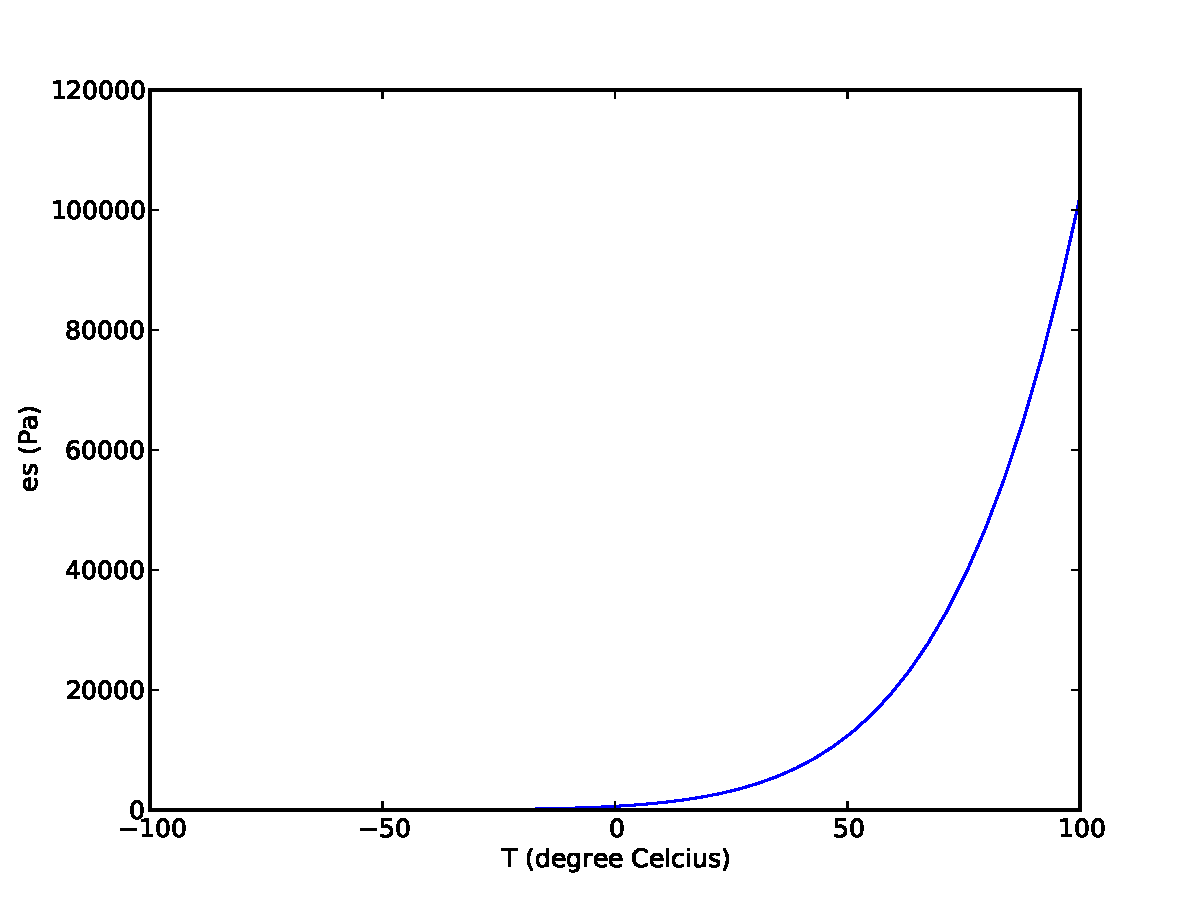
\includegraphics[width=0.5\textwidth]{images/es_t.pdf}
  \caption{The variation of saturation vapor pressure $(e_s)$ versus temperature $(T)$. }
  \label{fig:es_t}
\end{figure}
\afterfig

\section{Precipitation}
The terminal velocity $(V_t)$ of a falling raindrop is given by:
\begin{equation}
V_t = \left[\frac{4gD}{3C_d}\left( \frac{\rho_w}{\rho_a}-1\right) \right]^{1/2},
\end{equation}
where, $g$ is the acceleration due to gravity, $D$ is the diameter of the falling raindrop, $\rho_w$ is the density of water, $\rho_a$ is the density of air, and $C_d$ is the drag coefficient. The \emph{Stoke's law} can be used to calculate drag coefficient $(C_d = 24/Re)$, which is valid for raindrop having diameter less than 0.1 mm. $Re$ is the Reynold number, which can be calculated as $\rho_a VD/\mu_a$. Let us assume, that the $Re$ is given as 5.0, and the raindrop has diameter of 0.05 mm, and we want to estimate the $V_t$. ($\rho_w = 998$, $\rho_a=1.2$).
\beforeverb
\begin{verbatim}
>>> import numpy as np
>>> Re = 5.0; rho_w = 998; rho_a = 1.2; g = 9.8; D = 0.05E-3
>>> Cd = 24/Re
>>> Vt = np.sqrt((4*g*D)/(3*Cd)*(rho_w/rho_a-1))
>>> Vt
0.3362483649967134
\end{verbatim}
\afterverb
In this example we see that `\verb";"' allows us to define many expressions in one line.
\index{semicolon (;)}

\section{Rainfall}
Often, we are given a rainfall recorded by a rain gauge which provides the rainfall depths recorded for successive interval in time, and we want to compute the cumulative rainfall. In this example first we shall create rainfall using the random numbers, and we shall also create time variable having values [0,5,10, ...., 100]. 
\beforeverb \begin{verbatim}
>>> import numpy as np
>>> time = np.linspace(0,100,21) # create time variable
>>> time
array([   0.,    5.,   10.,   15.,   20.,   25.,   30.,   35.,   40.,
         45.,   50.,   55.,   60.,   65.,   70.,   75.,   80.,   85.,
         90.,   95.,  100.])
>>> rainfall = np.random.rand(21) # generate rainfall
>>> rainfall
array([ 0.08155645,  0.88821997,  0.33355457,  0.49600859,  0.6315054 ,
        0.0722053 ,  0.06165701,  0.96105307,  0.56483934,  0.5194715 ,
        0.35780167,  0.98950575,  0.67866578,  0.31274527,  0.80022389,
        0.53321842,  0.82370443,  0.73212013,  0.77039599,  0.06392391,
        0.53481488])
\end{verbatim} \afterverb

Now we make a bar plot using the \verb"plt.bar()", for the rainfall which depicts temporal behaviour of the rainfall. 
\beforeverb \begin{verbatim}
>>> import matplotlib.pyplot as plt
>>> plt.bar(time,rainfall)
>>> plt.xlabel('Time')
>>> plt.ylabel('Incremental rainfall')
>>> plt.savefig('/home/tomer/articles/python/tex/images/rain.png')
\end{verbatim} \afterverb
The resulted bar plot of rainfall is shown in Fig \ref{fig:rain}. You might have noticed that in the section 4.2, we used the \verb"plt.show()", while in the above example we used \verb"plt.savefig". The \verb"plt.show()" shows the graph on computer screen, which can be saved later, while the \verb"plt.savefig()" saves the graphs in computer, which can be viewed after opening the file. It is just matter of taste, what you like, optionally both can be done on same graph. I prefer to save the figures in the computer and then see them. 
\index{bar}

\beforefig
\begin{figure}[h!]
  \centering
    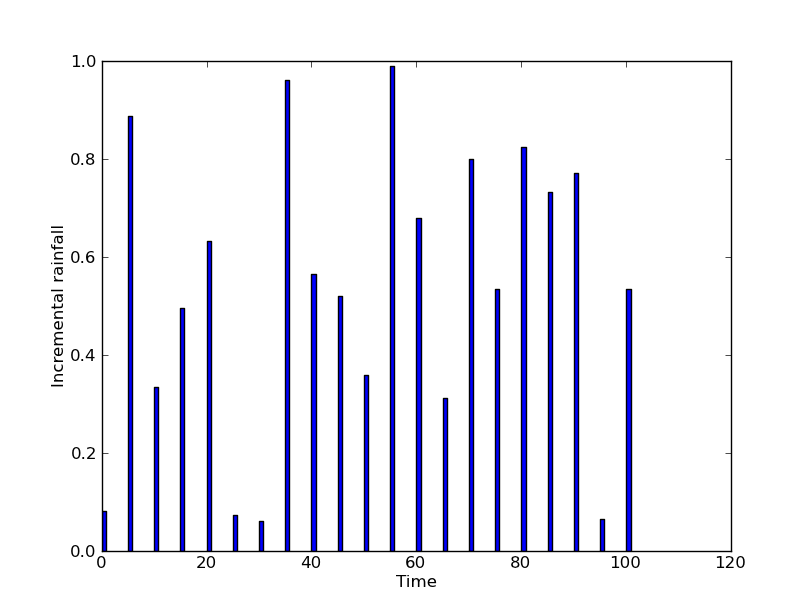
\includegraphics[width=0.5\textwidth]{images/rain.png}
  \caption{Temporal variation in the incremental rainfall. }
  \label{fig:rain}
\end{figure}
\afterfig

The cumulative sum is calculated by using the \verb"cumsum" function of the \verb"numpy" library. 
\beforeverb \begin{verbatim}
>>> cum_rainfall = np.cumsum(rainfall)
\end{verbatim} \afterverb
\index{cumsum}

Now we plot the cumulative rainfall. The resulted cumulative rainfall is shown in Fig. \ref{fig:cum_rain}. The \verb"plt.clf()" clears the current figure, and is quiet useful when making multiples plots, and there is any existing plot in the python memory. Just don't use the \verb"clf" in this, and see the difference. 
\beforeverb \begin{verbatim}
>>> plt.clf()
>>> plt.plot(time,cum_rainfall)
>>> plt.xlabel('Time')
>>> plt.ylabel('Cummulative rainfall')
>>> plt.savefig('/home/tomer/articles/python/tex/images/cum_rain.png')
\end{verbatim} \afterverb

\beforefig
\begin{figure}[h!]
  \centering
    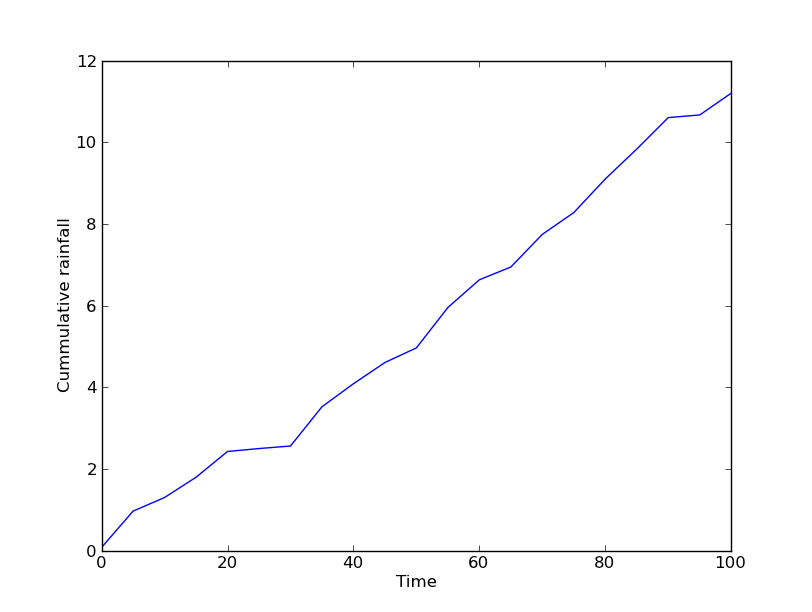
\includegraphics[width=0.5\textwidth]{images/cum_rain.png}
  \caption{Temporal behaviour of the cumulative rainfall . }
  \label{fig:cum_rain}
\end{figure}
\afterfig

Usually, we are given the rainfall at some rain gauges, and we want to make the isohyete (contour) plot of the rainfall. To demonstrate this situation, fist we shall generate locations  (x,y) and rainfall for ten stations using random numbers. The generated locations of the rain gauges is shown in Fig. \ref{fig:loc}. 
\beforeverb \begin{verbatim}
>>> # import required modules
>>> import numpy as np
>>> import matplotlib.pyplot as plt
>>> 
>>> #genrate locations and rainfall
>>> x = np.random.rand(10)
>>> y = np.random.rand(10)
>>> rain = 10*np.random.rand(10)
>>> 
>>> #plot the locations
>>> plt.scatter(x,y)
>>> plt.xlabel('X')
>>> plt.ylabel('Y')
>>> plt.savefig('/home/tomer/articles/python/tex/images/loc.png')
\end{verbatim} \afterverb
I prefer to add blank lines after a section of code, and comment on the top of section what it is doing. This increases the readability of the code. The \verb"plt.scatter()" makes the scatter plot, i.e. the dots are plotted instead of lines. When there is no order in the data with respect to their position in the array, then scatter plot is used. Like in this case, it is possible that two stations which are close by, but might be placed at distant in the array. 
\beforefig \begin{figure}[h!]
  \centering
    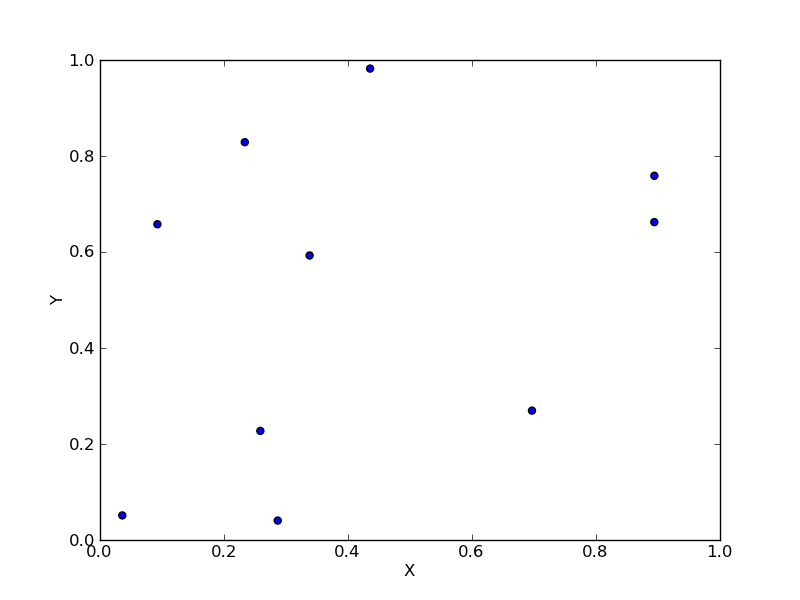
\includegraphics[width=0.5\textwidth]{images/loc.png}
  \caption{Spatial distribution of the rain gauges.}
   \label{fig:loc}
\end{figure}
\afterfig

% styles for flowcharts
\tikzstyle{decision} = [diamond, draw, text width=3cm, text badly centered, node distance=3cm, inner sep=0pt]
\tikzstyle{block} = [rectangle, draw, text width=3cm, text centered, rounded corners, minimum height=2em]
\begin{figure}
 \begin{center}
  \begin{tikzpicture}[node distance=4.5cm, auto, >=stealth]
   % nodes
   \node[block] (a)  				                    {Location of gauges};
   \node[]      (b)  [right of=a]                       {};
   \node[block] (c)  [right of=b]                       {Data (e.g. rainfall)};
   \node[block] (d)  [below of=b, node distance=2cm]  	{Interpolate};
   \node[block] (e)  [below of=d, node distance=2cm]  	{Gridded data};
   \node[block] (f)  [left of=d]    					{Regular grid with required extent and spacing};
   \node[block] (g)  [below of=e, node distance=2cm]    {Contour map};
      
   % edges
   \draw[->] (a) -- (d);
   \draw[->] (c) -- (d);
   \draw[->] (d) -- (e);
   \draw[->] (e) -- (g);
   \draw[->] (f) -- (d);
   \end{tikzpicture}
  \caption{Flowchart of making contour map from the data of rainfall gauges}
  \label{fig:flowchart}
 \end{center}
\end{figure}

The flow chart of preparing contour map is given in Fig. \ref{fig:flowchart}. First, we need to generate the grid with regular spacing having the same extent as of the locations of rainfall gauges. Then, from the given location and rainfall data, we need to compute data at regular grid using some interpolation scheme. After this contour maps can be obtained. The \verb"griddata" function of the \verb"scipy.interpolate" library is useful in obtaining the gridded data (data at regular grid). When we need only one or few functions from the library, it is better to call them explicitly, e.g. \verb"from scipy.interpolate import griddata", like in the following example. We use \verb"meshgrid" function of numpy library, to create the mesh from the given $x$ and $y$ vectors. 

\beforeverb \begin{verbatim}
>>> from scipy.interpolate import griddata
>>> #generate the desired grid, where rainfall is to be interpolated
>>> X,Y = np.meshgrid(np.linspace(0,1,1000), np.linspace(0,1,1000))
>>> 
>>> #perform the gridding
>>> grid_rain = griddata((x,y), rain, (X, Y))
\end{verbatim} \afterverb
\index{meshgrid}

Now, we can make the contour plot of the gridded data, which is made by \verb"plt.contourf()" function. The \verb"contourf" makes filled contours, while \verb"contour()" provides simple contour. Try using the \verb"contour" instead of \verb"contourf", and you will see the difference. We begin by clear current figure by using the \verb"plt.clf()", as there might be some existing figure in the memory especially if you are following all the examples in the same session. We are also overlaying the locations of rainfall gauges using the \verb"plt.scatter()". The \verb"s" and \verb"c" are used to define the size and color of the markers respectively. The \verb"plt.xlim()" and \verb"plt.ylim()" limits the extent of the $x$ and $y$ axis respectively. 
\beforeverb \begin{verbatim}
>>> plt.clf()
>>> plt.contourf(X,Y,grid_rain)
>>> plt.colorbar()
>>> plt.xlabel('X')
>>> plt.ylabel('Y')
>>> plt.scatter(x, y, s=30, c='r')
>>> plt.xlim((0,1))
>>> plt.ylim((0,1))
>>> plt.savefig('/home/tomer/articles/python/tex/images/grid_rain.png')
\end{verbatim} \afterverb
\index{contourf}
\index{colorbar}
\index{scatter}
\index{xlim}
\index{ylim}

Fig. \ref{fig:grid_rain} shows the gridded rainfall along with the location of rain gauges. The \verb"gridata" does not perform extrapolation, so the data outside the location of the rain gauges is assigned a value of \verb"nan". There are other function which can be used to extrapolate the data, which would be discussed later. 

\beforefig
\begin{figure}[h!]
  \centering
    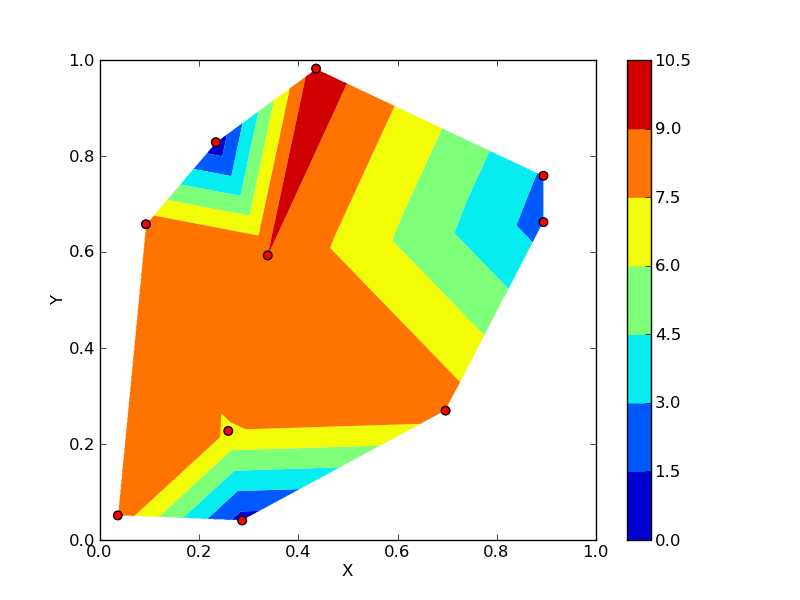
\includegraphics[width=0.5\textwidth]{images/grid_rain.png}
  \caption{Gridded rainfall along with the location of rain gauges.}
   \label{fig:grid_rain}
\end{figure}
\afterfig

\section{Evaporation}
Based on the energy balance, the evaporation rate  ($E_r$) after neglecting the sensible heat flux and ground heat flux, can be calculated as,
\begin{equation}
E_r = \frac{R_n}{l_v\rho_w},
\end{equation}
where, $R_n$ is the net radiation, $l_v$ is the latent heat of vaporization, and $\rho_w$ is the water density. The $l_v$ can be approximated as,
\begin{equation}
l_v = 2500 - 2.36\times T,
\end{equation}
where, $T$ is the temperature in Celcius. \\


Based on the aerodynamic, the evaporation rate ($E_a$) can be calculated as,
\begin{equation}
E_a = B\left(e_{as} - e_a\right),
\end{equation}
where,
\begin{equation}
B = \frac{0.622k^2 \rho_a u_2}{p \rho_w \left[\ln (z_2/z_0)\right]^2},
\end{equation}
$e_{as}$ is the saturated vapor pressure, $e_a$ is the vapor pressure, $k$ is the von Karnman coefficient, $u_2$ is wind velocity measured at $z_2$ m height, $p$ is the air pressure, and $z_0$ is the roughness height. \\

Usually, evaporation is calculated by combining the energy balance and aerodynamic method. In this case the $E$ becomes,
\begin{equation}
E = \frac{\Delta}{\Delta + \gamma} E_r + \frac{\gamma}{\Delta + \gamma}E_a,
\end{equation}
where, $\Delta$ is the gradient of the saturated vapor pressure curve, and is,
\begin{equation}
\Delta = \frac{4098 e_s}{(273.3+T)^2},
\end{equation}
and, the $\gamma$ is the psychrometric constant, and is defined as,
\begin{equation}
\gamma = \frac{C_p K_h p}{0.622 l_v K_w},
\end{equation}
$k_h$ and $k_w$ are the heat and vapor diffusivities respectively. \\

Let us first generate the synthetic data using random numbers. We know that \verb"np.random.rand" provides uniformly distributed random number over an interval of [0,1]. If we want to get the uniformly distributed random number over some other range, say [a,b], we can transform the variable in the following way:
\begin{equation}
x_{new} = a + (b-a)*x_{old},
\end{equation}
where, $X_{old}$ is uniformly distributed random variable over [0,1], and $x_{new}$ has the range of [a,b]. The \verb"np.random.randn" gives normally distributed random variables having zero mean and standard deviation equal to one. If we are interested in normally distributed random variable having mean $\mu$ and standard deviation equal to $\sigma$. We can do the following transformation.
\begin{equation}
y_{new} = \mu + \sigma*y_{old},
\end{equation}
where, $y_{new}$ is transformed variable having mean equal to $\mu$ and standard deviation equal to $\sigma$, and $y_{old}$ is the normally distributed random variable with mean zero and standard deviation equation to one, as generated by the \verb"np.random.randn" function. \\

In the following example, we shall generate variable in their usual range. The comment after the variable provides details of the lower and upper range in case of uniformly distributed random variable, mean and standard deviation when the variable is normally distributed. 

\beforeverb \begin{verbatim}
>>> from __future__ import division
>>> import numpy as np
>>> import matplotlib.pyplot as plt
>>> 
>>> # generate the synthetic data
>>> Rn = 150+100*np.random.rand(100) # lower bound = 150, upper boun = 250
>>> T = 25+3*np.random.randn(100) # mean = 25, std = 3
>>> Rh = 0.2+0.6*np.random.rand(100) # lower bound = 0.2, upper boun = 0.8
>>> u2 = 3+np.random.randn(100) # mean = 3, std = 1
>>> 
>>> # define constants
>>> rho_w = 997; rho_a = 1.19; p = 101.1e3; z2 = 2
>>> z0 = 0.03e-2; k = 0.4; Cp = 1005
\end{verbatim} \afterverb

Now, we apply the energy balance based method to estimate the evaporation. 
\beforeverb \begin{verbatim}
>>> lv = (2500-2.36*T)*1000 # multiplied by thousand to convert from KJ/kg to J/kg
>>> Er = 200/(lv*997)
>>> Er *= 1000*86400 # convert from m/s to mm/day
\end{verbatim} \afterverb
We are using multiplication and assignment operator to convert the units. We could have done this by simply multiplication also i.e. \verb"Er = Er*1000*86400". The multiplication and assignment operator is fast, as it does not create any temporary variable in the memory. In fact all the assignment operator are faster than simple operator, and should be used whenever there is scope to use them. Now we estimate the evaporation using the aerodynamic method.
\beforeverb \begin{verbatim}
>>> B = 0.622*k**2*rho_a*u2/(p*rho_w*(np.log(z2/z0))**2)
>>> e_s = 611*np.exp(17.27*T/(237.3+T))
>>> e_a = Rh*e_s
>>> Ea = B*(e_s-e_a)
>>> Ea *= 1000*86400 # convert from m/s to mm/day
\end{verbatim} \afterverb
Now, we combine energy balance and aerodynamic method to get improved estimate of the evaporation.
\beforeverb \begin{verbatim}
>>> gamma = Cp*p/(0.622*lv) # since kh/kw = 1, hence they are dropped form eq.
>>> delta = 4098*e_s/(237.3+T)**2
>>> w = delta/(delta+gamma)
>>> E = w*Er + (1-w)*Ea
\end{verbatim} \afterverb

\index{subplot}
Now, we have got four important variables; evaporation using energy balance method ($E_r$), evaporation using aerodynamics method ($E_a$), combined evaporation ($E$), and the ratio of evaporation from energy balance method by combined method ($Er/E$). We can plot these four variables in four different plot, or we can put them in one figure by making figure into four section. \verb"subplot" is such a function to make figure into subsection. The first argument to \verb"subplot" is the desired number of rows, second argument is the desired numbers of columns in the figure. The third argument is the position of subplot in the figure, which is measured from left to right and top to bottom. 
\beforeverb \begin{verbatim}
>>> plt.clf()
>>> plt.subplot(2,2,1)
>>> plt.plot(Er)
>>> plt.xlabel('Time')
>>> plt.ylabel('Er')

>>> plt.subplot(2,2,2)
>>> plt.plot(Ea)
>>> plt.xlabel('Time')
>>> plt.ylabel('Ea')

>>> plt.subplot(2,2,3, axisbg='y')
>>> plt.plot(E)
>>> plt.xlabel('Time')
>>> plt.ylabel('E')

>>> plt.subplot(2,2,4, axisbg='g')
>>> plt.plot(w)
>>> plt.xlabel('Time')
>>> plt.ylabel('Er/E')
>>> plt.savefig('/home/tomer/articles/python/tex/images/E.png')
\end{verbatim} \afterverb

The estimated $E_r$, $E_a$, $E$ and $Er/E$ are shown in the Fig. \ref{fig:E}. We have additionally used the argument \verb"axisbg" to define the background color for the subplots. 
\beforefig
\begin{figure}[h!]
  \centering
    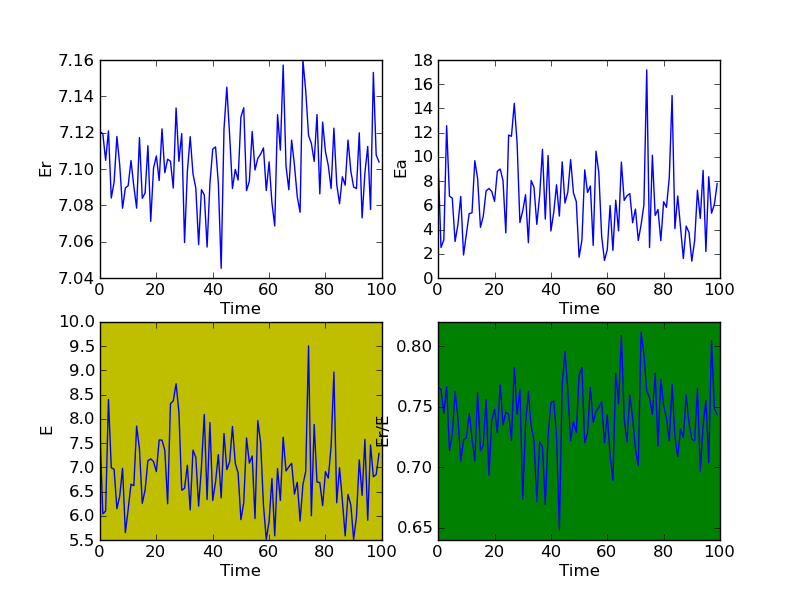
\includegraphics[width=0.5\textwidth]{images/E.png}
  \caption{The estimated $E_r$, $E_a$, $E$ and $Er/E$.}
   \label{fig:E}
\end{figure}
\afterfig

In the Fig. \ref{fig:E}, the \verb"ylabel" of subplot 4 is overlapping with the subplot 3. This can be corrected by changing the \verb"wspace". Which is demonstrated below. Fig. \ref{fig:corr_E} shows the improved plot.
\index{wspace}
\beforeverb
\begin{verbatim}
>>> fig = plt.figure()
>>> fig.subplots_adjust(wspace=0.6)
>>> plt.subplot(2,2,1)
>>> plt.plot(Er)
>>> plt.xlabel('Time')
>>> plt.ylabel('Er')
>>> 
>>> plt.subplot(2,2,2)
>>> plt.plot(Ea)
>>> plt.xlabel('Time')
>>> plt.ylabel('Ea')
>>> 
>>> plt.subplot(2,2,3, axisbg='y')
>>> plt.plot(E)
>>> plt.xlabel('Time')
>>> plt.ylabel('E')
>>> 
>>> plt.subplot(2,2,4, axisbg='g')
>>> plt.plot(w)
>>> plt.xlabel('Time')
>>> plt.ylabel('Er/E')
>>> plt.savefig('/home/tomer/articles/python/tex/images/corr_E.png')
\end{verbatim}
\afterverb

\beforefig
\begin{figure}[h!]
  \centering
    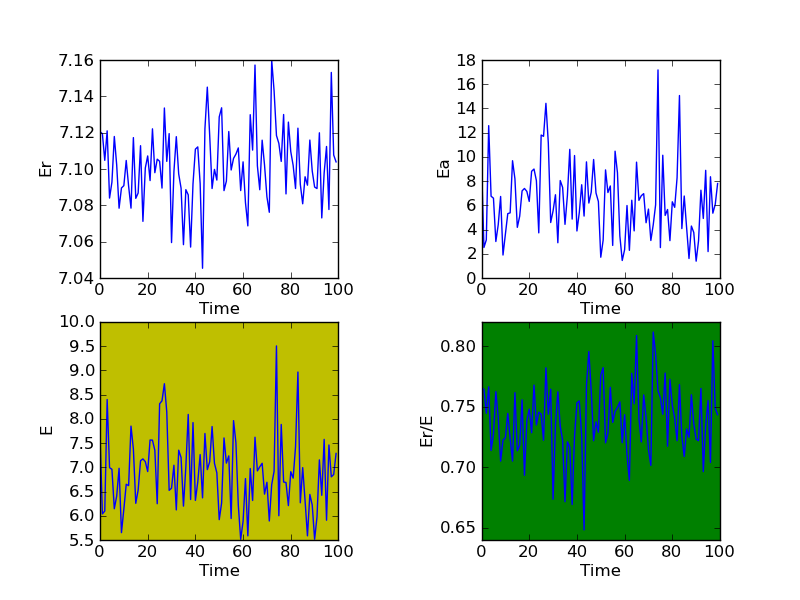
\includegraphics[width=0.5\textwidth]{images/corr_E.png}
  \caption{Estimated $E_r$, $E_a$, $E$ and $Er/E$ with corrected ylabel.}
   \label{fig:corr_E}
\end{figure}
\afterfig

\section{Infiltration}
The cumulative infiltration given by Green-Ampt method is written as,
\begin{equation}
\label{eq:infil}
F(t) - \psi \Delta \theta \ln \left(1 + \frac{F(t)}{\psi \Delta \theta} \right) = Kt,
\end{equation}
where, $F(t)$ is the cumulative infiltration after $t$ time, $\psi$ is the suction head , $\Delta \theta$ is given as,
\begin{equation}
\Delta \theta = (1-S_e) \theta_e,
\end{equation}
wherein, $S_e$ is the degree of saturation, and $\theta_e$ is the effective porosity, $K$ is the hydraulic conductivity. To solve the equation using iterative procedure, the Eq. \ref{eq:infil} is rewritten as,
\begin{equation}
F(t) = \psi \Delta \theta \ln \left(1 + \frac{F(t)}{\psi \Delta \theta} \right) + Kt.
\end{equation}

We use \verb"while" function to iterate till we achieve required accuracy. The iterated value of $F$ are stored using the \verb"append" method. \verb"append" appends the array by one one item, and puts the input variable into it. 
\index{\_\_future\_\_}
\beforeverb \begin{verbatim}
>>> from __future__ import division
>>> import numpy as np

>>> # define the variables
>>> theta_e = 0.486
>>> psi = 16.7
>>> K = 0.65
>>> S_e = 0.3
>>> t = 1
>>> 
>>> #calculate dtheta
>>> dtheta = (1-S_e)*theta_e
>>> 
>>> # initial guess of F
>>> F_old = K*t
>>> epsilon = 1
>>> F = []
>>> while epsilon > 1e-4:
>>>     F_new = psi*dtheta * np.log(1+F_old/(psi*dtheta)) + K*t
>>>     epsilon = F_new - F_old
>>>     F_old = F_new
>>>     F.append(F_new)
\end{verbatim} \afterverb

Now, we make a plot of the iterated value of $F$ to see how $F$ is getting updated with iterations. We are also using \verb"-ok" in the \verb"plot" function. The \verb"-o" represents the continuous line with filled dots, and \verb"k" tells that the color of plot is black. We are also specifying the font size for \verb"xlabel" and \verb"ylabel". We have used `25' for \verb"ylabel" and `20' for \verb"xlabel", just to demonstrate that different font sizes can be used for different texts. Of course, there is no need to define a different font size for \verb"ylabel" and \verb"xlabel". The same argument \verb"fontsize" can be used to define the font size for legend also. 

\beforeverb \begin{verbatim}
>>> import matplotlib.pyplot as plt
>>> plt.plot(F,'-ok')
>>> plt.xlabel('Number of iteration',fontsize=25)
>>> plt.ylabel('F',fontsize=20)
>>> plt.savefig('/home/tomer/articles/python/tex/images/F.png')
\end{verbatim} \afterverb

\beforefig
\begin{figure}[h!]
  \centering
    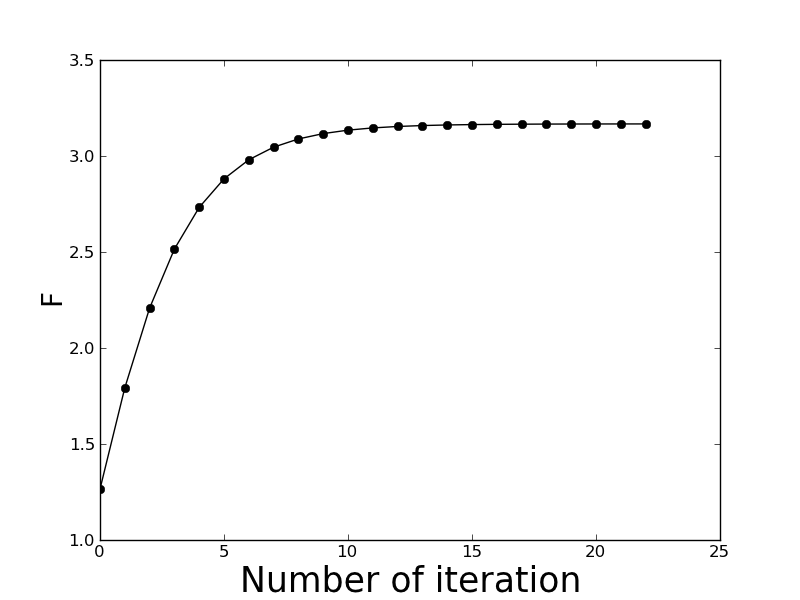
\includegraphics[width=0.5\textwidth]{images/F.png}
  \caption{The variation of the $F$ with iterations.}
   \label{fig:F}
\end{figure}
\afterfig

Fig. \ref{fig:F} shows the variation of the $F$ over time. The $F$ is becoming almost constant after approximately 12 iterations. 

\section{Surface water}
The flow depth in a rectangular channel is given by,
\begin{equation}
Q = \frac{1.49}{n}S_o^{1/2}\frac{(By)^{5/3}}{(B+y)^{2/3}},
\end{equation}
where, $Q$ is the flow, $n$ is the Manning's coefficient, $S_0$ is slope of water surface, $B$ is the width of channel, and $y$ is the flow depth. This is a nonlinear equation in $y$, and the explicit solution of this is not yet found. This can be solved iteratively like in the last section, or using methods like Newton-Raphson. In this, we will solve using the \verb"fmin" function of the \verb"Scipy.optimize" library. First we will import required libraries. Then we will define a function that takes the flow depth $(y)$ as input and gives the error in the flow estimated based on this $y$ and the given $Q$. We are taking absolute value of error, other options are like square of error etc. After specifying the function, we can give this function as a input to \verb"fmin" and some initial guess of the $y$.  
\index{fmin}
\beforeverb \begin{verbatim}
>>> # import required modules
>>> from __future__ import division
>>> import numpy as np
>>> import matplotlib.pyplot as plt
>>> from scipy.optimize import fmin
>>> 
>>> # define the variables
>>> n = 0.015
>>> S0 = 0.025
>>> Q = 9.26
>>> B = 2
>>> 
>>> # define the flow function
>>> def flow(y):
>>>     Q_estiamted = (1.49/n)*(S0**0.5)*((B*y)**(5/3))/((B+y)**(2/3))
>>>     epsilon = np.abs(Q_estiamted - Q)
>>>     return epsilon
>>> 
>>> y_optimum = fmin(flow,0.5)
\end{verbatim} \afterverb
\verb"fmin" will give us the required $y$ value. We can also get details of the iterations, and error value at final iterations. We use \verb"print" function to see the details. The output is given below. 
\beforeverb \begin{verbatim}
>>> print(y_optimum)
Optimization terminated successfully.
         Current function value: 0.000078
         Iterations: 13
         Function evaluations: 26
[ 0.52770386]
\end{verbatim} \afterverb
The optimization terminated successfully, i.e. the required accuracy was achieved within the default maximum number of iterations allowed. The output tells that it took 13 iterations to achieve the required accuracy, and that the function was evaluated 26 times in the process. 

\section{River Routing--Muskingum method}
The outflow using Muskingum method is calculated as,
\begin{equation}
Q_{j+1} = C_1 I_{j+1} + C_2 I_j + C_3 Q_j.
\end{equation}
We are given the value of $C_1$, $C_2$, $C_3$, and $Q_0$, and we are interested in getting the value of $Q$ from time ($t=0$) to ($t=19$). In this example, first we define variables, and then we iterate using \verb"for" loop. The list \verb"I" is quiet long, and will not fit into one line. In such cases we can go to second line also, the beginning of brackets tells Python that list has started, and the end brackets tells Python that this is end of the list. We can write list in as many line as we want, no need to specify anything else to tell Python that list is defined in multi-line. 
\beforeverb \begin{verbatim}
>>> from __future__ import division
>>> import numpy as np
>>> # define the variables
>>> I = np.array([93, 137, 208, 320, 442, 546, 630, 678, 691, 675, 634, 571, 477, 
>>>               390, 329, 247, 184, 134, 108, 90])
>>> C1 = 0.0631
>>> C2 = 0.3442
>>> C3 = 0.5927
>>> 
>>> Q = np.empty(20) # define the empty array
>>> Q[0] = 85 # initial value of Q
>>> 
>>> # loop over
>>> for i in range(1,20):
>>>     Q[i] = C1*I[i] + C2*I[i-1] + C3*Q[i-1] 
\end{verbatim} \afterverb

Now we can use \verb"matplotlib.pyplot" to plot the inflow and outflow. \verb"-*" means a continuous line with starts, and \verb"--s" means dashed line with square. 
\beforeverb \begin{verbatim}
>>> import matplotlib.pyplot as plt
>>> plt.plot(I, '-*', label='Inflow')
>>> plt.plot(Q, '--s', label='Outflow')
>>> plt.xlabel('Time', fontsize=20)
>>> plt.ylabel('Flow', fontsize=20)
>>> plt.legend()
>>> plt.savefig('/home/tomer/articles/python/tex/images/muskingum.png')
\end{verbatim} \afterverb

\beforefig
\begin{figure}[h!]
  \centering
    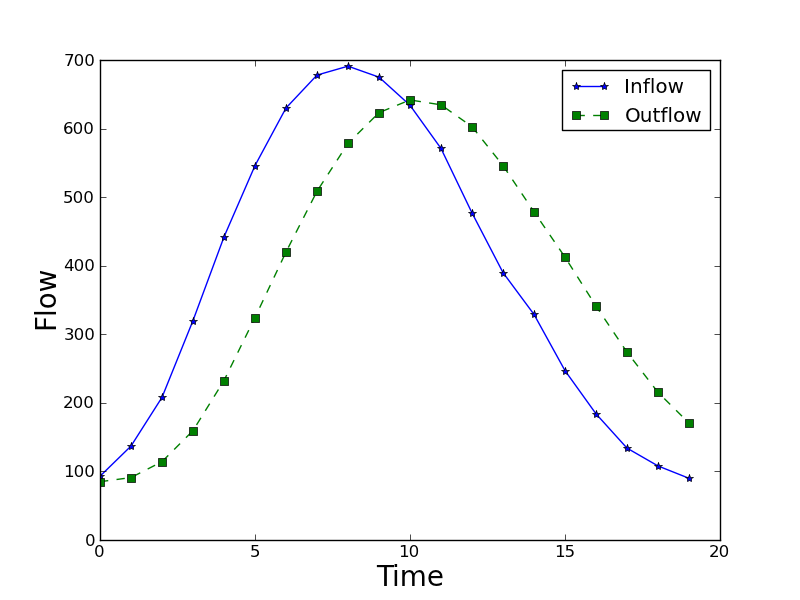
\includegraphics[width=0.5\textwidth]{images/muskingum.png}
  \caption{The variation of inflow and outflow with time.}
   \label{fig:musk}
\end{figure}
\afterfig

Fig. \ref{fig:musk} shows the variation of inflow and outflow with time. The outflow shows a lag with respect to inflow, and the peak in the outflow is slightly lesser than the inflow.

\chapter{Statistics}
When there is not a clear understanding of the physics process, or the variables required to do physical modelling are not available, then statistics plays a vital role. There are various modules available in python to deal with statistics, the most commonly used is \verb"scipy.stats". Additionally there is one more useful modules \verb"statistics", which can be downloaded from \url{http://bonsai.hgc.jp/~mdehoon/software/python/}. \verb"statistics" is not available for download using the \verb"pip", and hence you should download it using internet browser, and then install it using either \verb"pip" or \verb"python setup.py install". 

\section{Empirical distributions}
Most of hydrological variables are continuous, but because of our measurement capability we measure them discretely. The classification of discrete data using bins, provides mean to treat the discrete data as continuous. Visualization of the underlying distribution of data is done by plotting the Histogram.  The histogram depicts the frequency over discrete intervals (bins). So let us begin with histogram. In the following example, first we will generate some synthetic data, and then compute and plot the histogram. 

\beforeverb \begin{verbatim}
>>> from __future__ import division
>>> import numpy as np
>>> import matplotlib.pyplot as plt
>>> import scipy.stats as st
>>> 
>>> x = np.random.randn(100) # generate some synthetic data
>>> 
>>> # compute histogram
>>> n, low_range, binsize, extrapoints = st.histogram(x)
>>> upper_range  = low_range+binsize*(len(n)-1)
>>> bins = np.linspace(low_range, upper_range, len(n))
\end{verbatim} \afterverb
The \verb"st.histogram" provides the number of bins in each interval (n), lower range of the bin (low\_range), width of the bins (binsize), and points not used in the calculation of histogram. Since bin size is same for all bins, Python provides only one bin size. We used lower range of bin and bin size to first compute the upper range of the bin, and then compute the mid value for all the bins. Now we can use \verb"bar" to make the histogram. We shall also define the width and color of the bars. 
\index{histogram}
\beforeverb \begin{verbatim}
>>> plt.bar(bins, n, width=0.4, color='red')
>>> plt.xlabel('X', fontsize=20)
>>> plt.ylabel('number of data points in the bin', fontsize=15)
>>> plt.savefig('/home/tomer/articles/python/tex/images/hist.png')
\end{verbatim} \afterverb

The histogram of the data is shown in Fig. \ref{fig:hist}. In this example, because we have just created 100 random number from the normal distribution, the histogram is not showing the behaviour that normal distribution should show.  

\beforefig
\begin{figure}[h!]
  \centering
    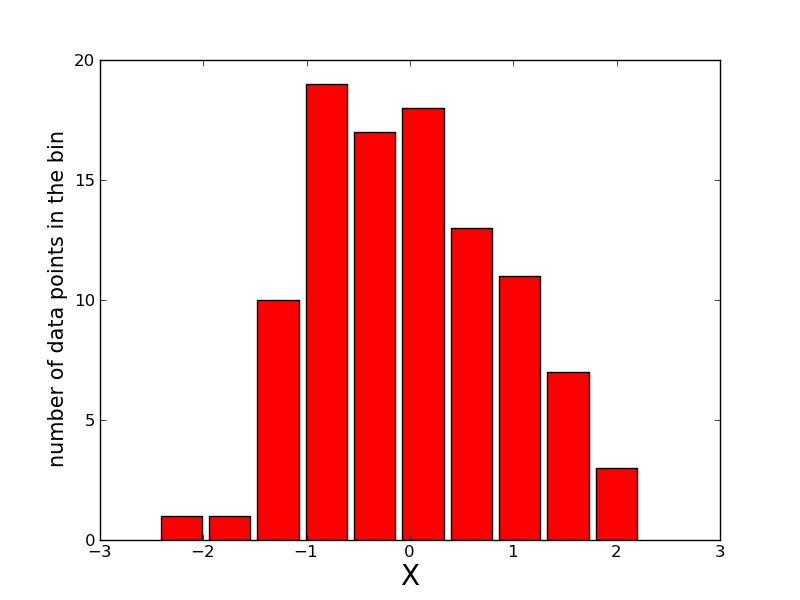
\includegraphics[width=0.5\textwidth]{images/hist.png}
  \caption{The Histogram of $x$.}
   \label{fig:hist}
\end{figure}
\afterfig

Each bar in histogram tells us that how many time the data was in particular bin. A better way to look at the behaviour of data is to look into relative histogram, which tells us about the probability with which data was in some range. The relative histogram or relative frequency is obtained by dividing the frequency in each bin by the sum of frequencies in all the bins. The relative histogram represents the probability of data occurring in the bins. Either we can use the \verb"histogram" function to first compute histogram, and then divide by total number of frequency, or we can directly use the \verb"relfreq" function. \verb"relfreq" provides the relative frequency, along with other output which are similar to that of \verb"histogram".
\index{relfreq}
\beforeverb \begin{verbatim}
>>> relfreqs, lowlim, binsize, extrapoints = st.relfreq(x)
>>> plt.bar(bins, relfreqs, width=0.4, color='magenta')
>>> plt.xlabel('X', fontsize=20)
>>> plt.ylabel('Relative frequencies', fontsize=15)
>>> plt.savefig('/home/tomer/articles/python/tex/images/relfreq.png')
\end{verbatim}
\afterverb
Because we are using the same $x$ that was used in previous example, hence we are not re-calculating the \verb"bins". In this bar plot, we are using \verb"magenta" color. The different color of plot, is just to make you familiar with colors and font sizes. And, it does not mean that we should use different color for relative frequency diagram than the histogram; nothing prevents us from using the same color.

\beforefig
\begin{figure}[h!]
  \centering
    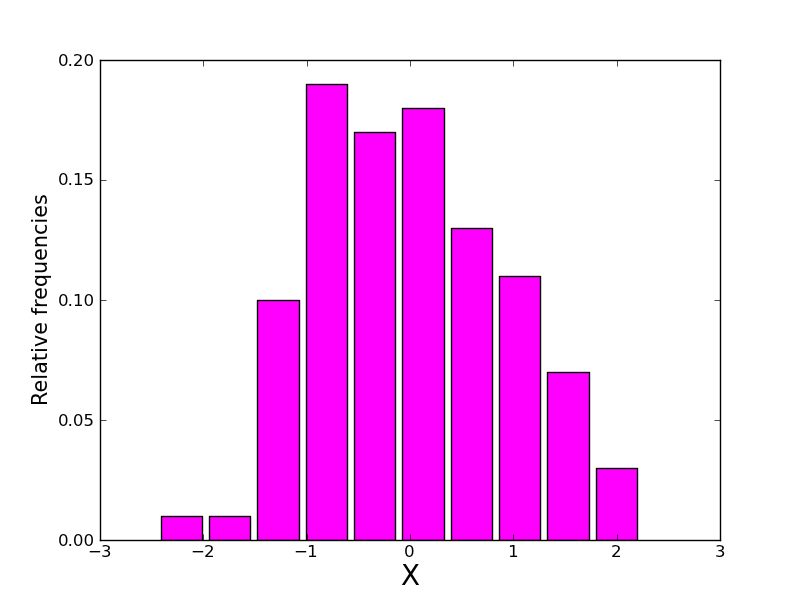
\includegraphics[width=0.5\textwidth]{images/relfreq.png}
  \caption{The relative histogram of $x$.}
   \label{fig:rf}
\end{figure}
\afterfig

The relative histogram is shown in Fig. \ref{fig:rf}. The relative histogram tells us how experimental data behaves; how many times (or with what probability) the data was in some range. The relative histograms only tell about experimental data, about the data we have. What about the data we are going to get into future? The PDF is a better indicator to say something about the future data. The probability density function (pdf) of a random variable is a function that describes the relative likelihood for this random variable to occur at a given point. The probability for the random variable to fall within a particular region is given by the integral of this variable’s density over the region. The probability density function is non-negative everywhere, and its integral over the entire space is equal to one. We can divide the relative frequency by the bin size, and get the pdf. A simple way to compute pdf is to use \verb"hist" function. \verb"hist" generates the plot, and also returns the value of pdf over 
each bin. The number of bins are controlled by giving second argument, in the following example it is set at 10. The \verb"bins" provide the lower and upper ranges of the bin, hence its length is one extra than the number of bins. Apart from the color we are specifying alpha value to \verb"hist" function. \verb"alpha" value controls the transparency of the plot; 0.0 means fully transparent and 1.0 is fully opaque. Fig. \ref{fig:pdf} shows the bar plot of the PDF. 
\index{PDF}
\beforeverb \begin{verbatim}
>>> n, bins, patches = plt.hist(x, 10, normed=1, facecolor='yellow', alpha=0.5)
>>> plt.xlabel('X', fontsize=15)
>>> plt.ylabel('PDF', fontsize=15)
>>> plt.savefig('/home/tomer/articles/python/tex/images/pdf.png')
\end{verbatim}
\afterverb

\beforefig
\begin{figure}[h!]
  \centering
    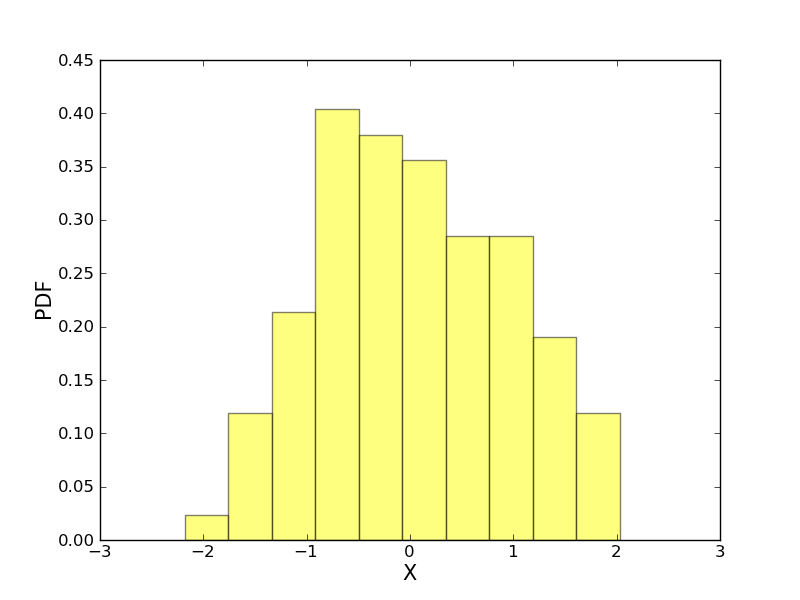
\includegraphics[width=0.5\textwidth]{images/pdf.png}
  \caption{The pdf of $x$.}
   \label{fig:pdf}
\end{figure}
\afterfig

The cumulative distribution function (CDF) describes the probability that a real-valued random variable $X$ with a given probability distribution will be found at a value less than or equal to $x$. \verb"cumfreq" provides cumulative frequency of the data, which can be used to compute the CDF. If we divide cumulative frequency by the total frequency, we get the CDF. The last value of cummulative frequency is equal to the total frequency, hence we are using this to compute CDF. The CDF is shown in Fig. \ref{fig:cdf}. 
\index{CDF}
\beforeverb \begin{verbatim}
>>> cumfreqs, lowlim, binsize, extrapoints = st.cumfreq(x)
>>> plt.bar(bins[:-1], cumfreqs/cumfreqs[-1], width=0.4, color='black', alpha=0.45)
>>> plt.xlabel('X', fontsize=15)
>>> plt.ylabel('CDF', fontsize=15)
>>> plt.savefig('/home/tomer/articles/python/tex/images/cdf.png')
\end{verbatim} \afterverb

\beforefig
\begin{figure}[h!]
  \centering
    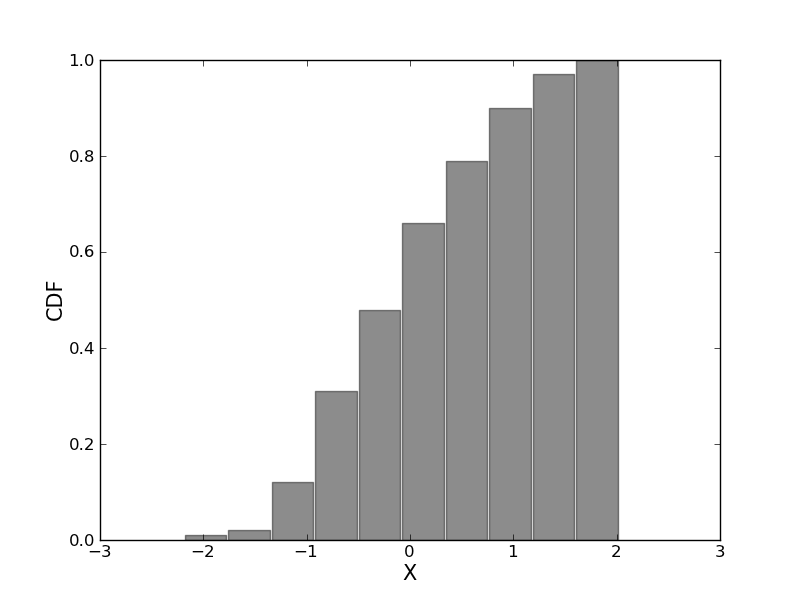
\includegraphics[width=0.5\textwidth]{images/cdf.png}
  \caption{The CDF of $x$.}
   \label{fig:cdf}
\end{figure}
\afterfig

We can use \verb"ECDF" function of the \verb"scikits" library to directly estimate the empirical cumulative distribution function (ECDF). The information about \verb"scikits" is give at \url{http://pypi.python.org/pypi/scikits.statsmodels}. The empirical distribution function (CDF) is the cumulative distribution function associated with the empirical measure of the sample. This cdf is a step function that jumps up by $1/n$ at each of the $n$ data points. The empirical distribution function estimates the underlying cdf of the points in the sample. In the previous example, we have estimated CDF (ECDF) after classifying data into some bins. This means, we assumed that the data behaves in a statistical similar way over some small range. We can estimate CDF without making this assumption also, which would be done using \verb"ECDF" function. The output form \verb"ECDF" function is a object which store the value of data and their corresponding ECDF. The data is retrieved using \verb"ecdf.x" and their corresponding 
ECDF is retrieved using \verb"ecdf.y". The \verb"ecdf" is the name of variable that you have defined to store the output of \verb"ECDF" function, if you use some other name, you need to use same name to retrieve \verb"x" and \verb"y" attributes. 
\index{ECDF}
\beforeverb \begin{verbatim}
>>> import numpy as np
>>> import scikits.statsmodels.api as sm
>>> import matplotlib.pyplot as plt
>>> 
>>> # generate some data
>>> data = np.random.randn(100)
>>> 
>>> # estimate ecdf
>>> ecdf = sm.tools.tools.ECDF(data)
\end{verbatim} \afterverb

We should plot ECDF as a step plot, because every ECDF is over some small interval. The ECDF plot is shown in Fig. \ref{fig:ecdf}. 
\beforeverb \begin{verbatim}
>>> plt.step(ecdf.x, ecdf.y)
>>> plt.xlabel('data', fontsize=20)
>>> plt.ylabel('Empirical CDF', fontsize=15)
>>> plt.savefig('/home/tomer/articles/python/tex/images/ecdf.png')
\end{verbatim} \afterverb

We can also use \verb"ecdf" to evaluate ECDF at any value of data. Let us evaluate and print value of ECDF at some data point (say at 0).
\beforeverb \begin{verbatim}
>>> print(ecdf(0))
0.48999999999999999
\end{verbatim} \afterverb

\beforefig
\begin{figure}[h!]
  \centering
    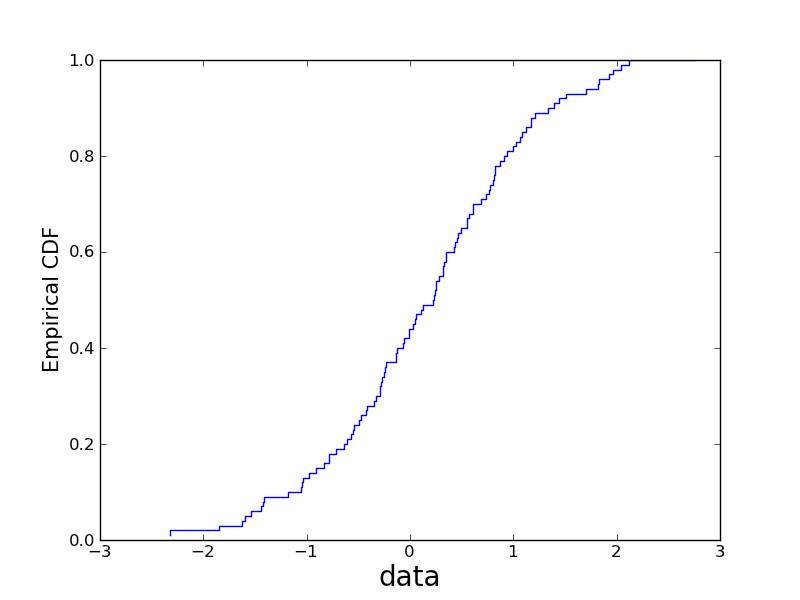
\includegraphics[width=0.5\textwidth]{images/ecdf.png}
  \caption{The empirical CDF estimated using ordinary method.}
   \label{fig:ecdf}
\end{figure}
\afterfig
\index{Kernel estimates}
The empirical CDF estimated using the method mentioned above results in the step function, which does not look so nice. A better way of estimating ECDF is by using kernel functions. This can be done by \verb"statistics" module. The \verb"statistics" library provides functions to estimate PDF and CDF using various kernel functions. \verb"cpdf" function is used for estimating CDF. We have also defined the name of kernal (Epanechnikov). The available kernal are given at website of library. Inside \verb"legend" we are defining location (loc) of the legend as \verb"best", which means Python will try to put the legend in the way, as to minimize the interference with plot. The resulted graph after using this curve is shows in Fig. \ref{fig:kernel}. It is evident from this figure, that this shows a smoother variation compared to ordinary method of ECDF estimation. 

\beforeverb
\begin{verbatim}
>>> import statistics
>>> y,x = statistics.cpdf(data, kernel = 'Epanechnikov') 
>>> plt.plot(ecdf.x, ecdf.y, label='Ordinary')
>>> plt.plot(x, y, label='Kernel')
>>> plt.xlabel('data', fontsize=20)
>>> plt.ylabel('Empirical CDF', fontsize=15)
>>> plt.legend(loc='best')
>>> plt.savefig('/home/tomer/articles/python/tex/images/kernel.png')
\end{verbatim}
\afterverb

\beforefig
\begin{figure}[h!]
  \centering
    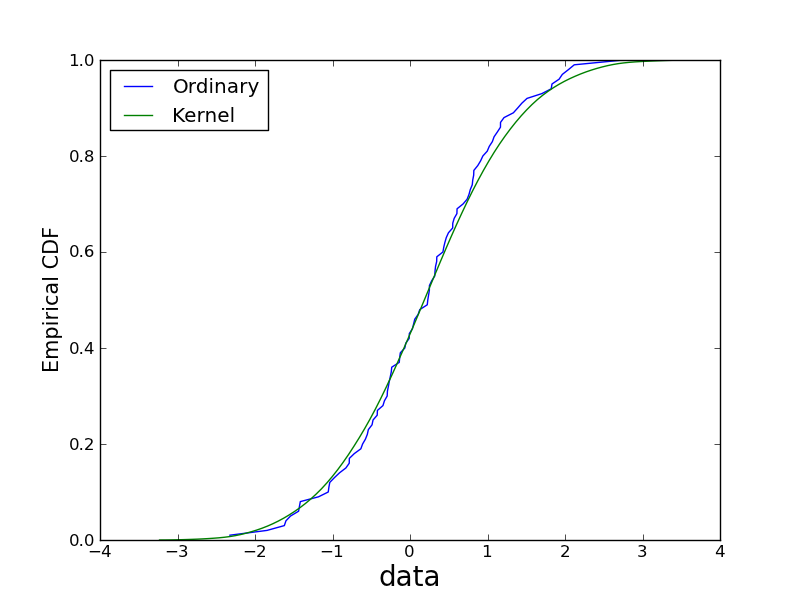
\includegraphics[width=0.5\textwidth]{images/kernel.png}
  \caption{Comparison of the ECDF estimated using ordinary method and based on kernal functions.}
   \label{fig:kernel}
\end{figure}
\afterfig

\section{Theoretical distributions}
Theoretical distributions are based upon mathematical formulas rather than empirical observations. There are various types of theoretical distributions, commonly used in hydrology are: Normal, Uniform, Exponential, Chi, Cauchy. The parameters of distributions are termed as location, scale, and shape parameter. The location parameter is the one, who change the location of pdf without affecting other attributes. Shape parameter is the one, who change the shape of distribution  without affecting other attributes. The parameter which stretch or shrink the distribution is called the scale parameters. 

First we will generate normally distributed random variables. The input required for this are location and scale parameter, which are mean and standard deviation in case of normal distribution. We can also use \verb"np.random.randn" to generate normally distributed random variables, but \verb"scipy.stats" provides many other utilities (methods). So we shall use \verb"scipy.stats" library. 

\beforeverb \begin{verbatim}
>>> import numpy as np
>>> import matplotlib.pyplot as plt
>>> import scipy.stats as st
>>> 
>>> # generate instances of normaly distributed random variable
>>> rv1 = st.norm(loc=0, scale=5)
>>> rv2 = st.norm(loc=0, scale=3)
>>> rv3 = st.norm(loc=0, scale=7)
\end{verbatim} \afterverb
\index{Distribution, normal}
Now these instances of variables can be used to evaluate PDF at any value. In the following example, we are computing pdf from -50 to 50 for plotting purpose. 

\beforeverb \begin{verbatim}
>>> x = np.linspace(-50,50, 1000)
>>> y1 = rv1.pdf(x)
>>> y2 = rv2.pdf(x)
>>> y3 = rv3.pdf(x)
\end{verbatim} \afterverb

Now, we have estimated PDF, it can be plotted. On the $x-axis$ we will keep the variable, and on the $y-axis$ keep the PDF. We are also supplying additional argument \verb"lw" to \verb"plot" function, which represents \verb"line width", and is used to control the widths of the plot. Fig. \ref{fig:pdf_norm} shows the PDF for three normally distributed random variables with varying scale parameters. The figure illustrates the effect of scale parameter on the PDF. In case of less scale parameter, more mass of pdf is concentrated in the center, as the scale parameter is increasing, the spread is increasing. 
\beforeverb \begin{verbatim}
>>> plt.plot(x, y1, lw=3, label='scale=5')
>>> plt.plot(x, y2, lw=3, label='scale=3')
>>> plt.plot(x, y3, lw=3, label='scale=7')
>>> plt.xlabel('X', fontsize=20)
>>> plt.ylabel('PDF', fontsize=15)
>>> plt.legend()
>>> plt.savefig('/home/tomer/articles/python/tex/images/norm_pdf.png')
\end{verbatim} \afterverb

\beforefig
\begin{figure}[h!]
  \centering
    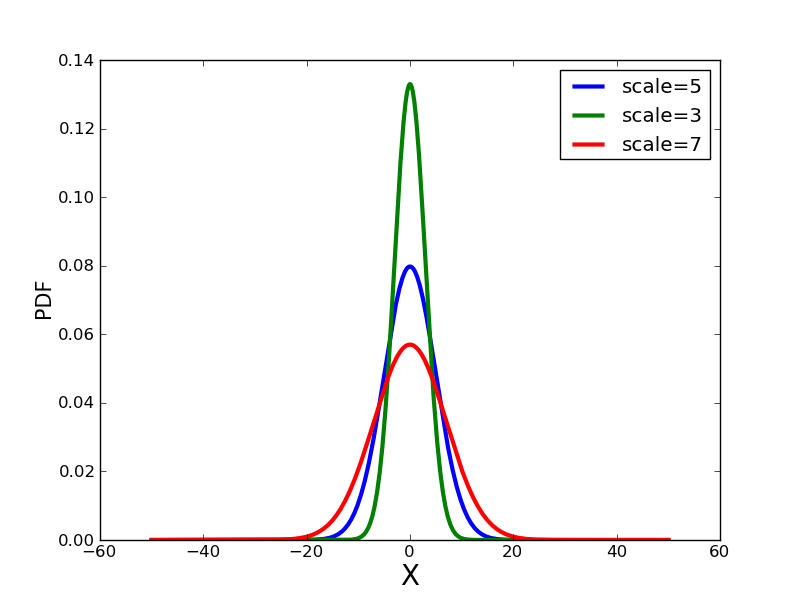
\includegraphics[width=0.5\textwidth]{images/norm_pdf.png}
  \caption{PDF for normal distribution with various scale parameter.}
   \label{fig:pdf_norm}
\end{figure}
\afterfig

We can use same instance to also get the CDF. The \verb"cdf" method gives the CDF at given input, which could be a scalar or an array. The CDF is shown in Fig. \ref{fig:cdf_norm}. CDF also shows the effect of scale parameter, but PDF provides a better inside. Hence it is always better to plot PDF to see the behaviour of the distribution or of the empirical data. 

\beforeverb \begin{verbatim}
>>> y1 = rv1.cdf(x)
>>> y2 = rv2.cdf(x)
>>> y3 = rv3.cdf(x)
>>> 
>>> # plot the pdf
>>> plt.clf()
>>> plt.plot(x, y1, lw=3, label='scale=5')
>>> plt.plot(x, y2, lw=3, label='scale=3')
>>> plt.plot(x, y3, lw=3, label='scale=7')
>>> plt.xlabel('X', fontsize=20)
>>> plt.ylabel('PDF', fontsize=15)
>>> plt.legend()
>>> plt.savefig('/home/tomer/articles/python/tex/images/norm_cdf.png')
\end{verbatim} \afterverb

\beforefig
\begin{figure}[!h]
  \centering
    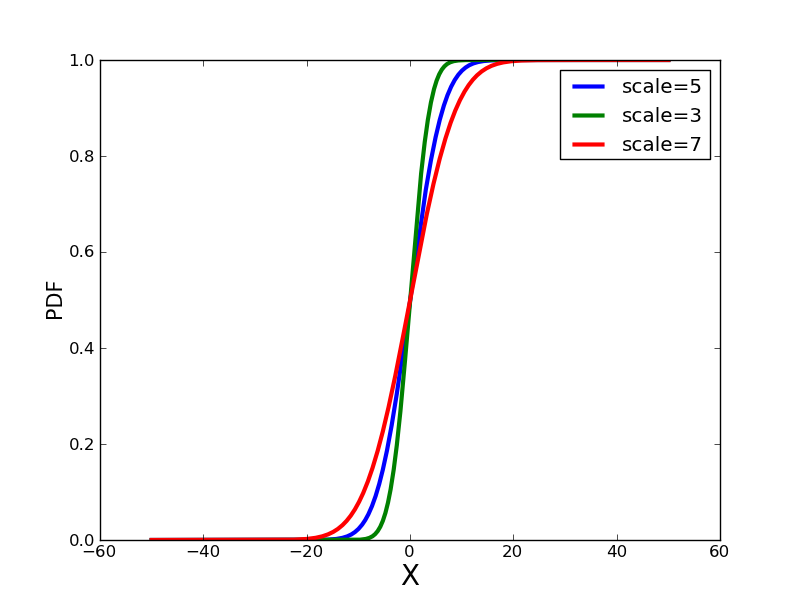
\includegraphics[width=0.5\textwidth]{images/norm_cdf.png}
  \caption{CDF of normal distribution for various scale parameter.}
   \label{fig:cdf_norm}
\end{figure}
\afterfig

There are other quiet commonly used distributions in hydrology, e.g. Cauchy, Chi, Exponential and Uniform etc. Let us, play with them also. First we will generate instance of these distributions. Chi distribution also require degree of freedom parameter apart from the location and scale parameters. In case of uniform distribution, the location parameter is defined as lower range, and scale parameter is defined as upper range, which is not true mathematically, and is defined just to make things easier in providing input to function. Fig.\ref{fig:pdf_all} shows the PDF for these distribution. 
\index{Distribution, Cauchy}
\index{Distribution, Chi}
\index{Distribution, Exponential}
\index{Distribution, Uniform}

\beforeverb \begin{verbatim}
>>> rv1 = st.cauchy(loc=0, scale=5)
>>> rv2 = st.chi(2, loc=0, scale=8)
>>> rv3 = st.expon(loc=0, scale=7)
>>> rv4 = st.uniform(loc=0, scale=20)
>>> 
>>> # compute pdf 
>>> y1 = rv1.pdf(x)
>>> y2 = rv2.pdf(x)
>>> y3 = rv3.pdf(x)
>>> y4 = rv4.pdf(x)
>>> 
>>> # plot the pdf
>>> plt.plot(x, y1, lw=3, label='Cauchy')
>>> plt.plot(x, y2, lw=3, label='Chi')
>>> plt.plot(x, y3, lw=3, label='Exponential')
>>> plt.plot(x, y4, lw=3, label='Uniform')
>>> plt.xlabel('X', fontsize=20)
>>> plt.ylabel('PDF', fontsize=15)
>>> plt.legend()
>>> plt.savefig('/home/tomer/articles/python/tex/images/pdf_all.png')
\end{verbatim}
\afterverb

\beforefig
\begin{figure}[h!]
  \centering
    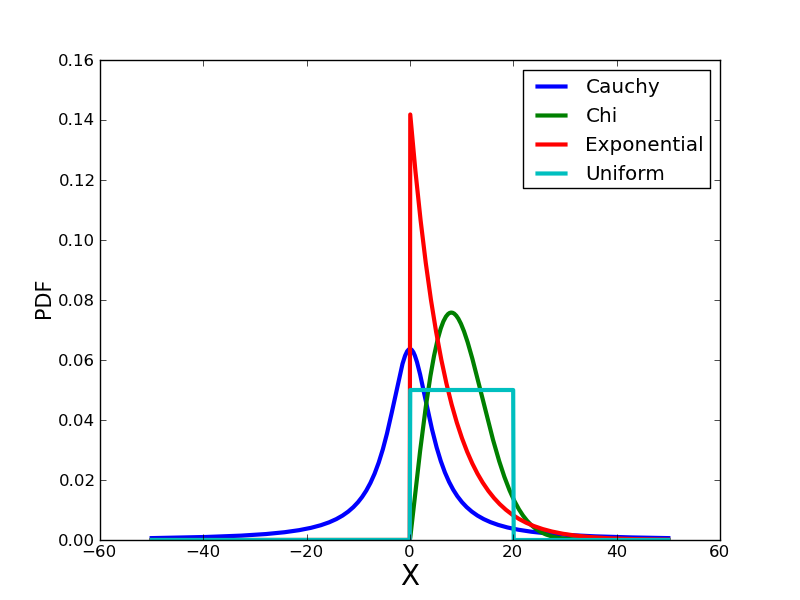
\includegraphics[width=0.5\textwidth]{images/pdf_all.png}
  \caption{PDF for various distributions.}
   \label{fig:pdf_all}
\end{figure}
\afterfig

We generate a number of random variable from some distribution to represent the distribution. To explore the impact of the number of samples on the empirical distribution, we will generate random number from same distribution but with various number of samples, and see how it is effecting the empirical distribution. We will not be using any quantitative measure to check this, as till this stage we have not talked about them, rather we will just visualize graphically. First we will play with normal distribution which is most commonly used distribution. We will use \verb"hist" function of the \verb"matplotlib.pyplot" library to compute the PDF. We are specifying \verb"normed=1" for the \verb"hist" function, which means that the area of histogram should be made equal to one, and which happens to be the PDF. We are also using \verb"plt.axis" to specify the limits of the plot, and we are keeping it same so that we can compare plots easily. The argument for \verb"plt.axis" are $[x_{min}, x_{max}, y_{min}, y_{max}]
$.  Fig. \ref{fig:pdf_norm_n} shows the empirical and theoretical PDF for sample equal to 100, 1000, 10,000, and 100,000. It is clear from the figure that as the number of sample are increasing, the empirical distribution is approaching near to theoretical one. At 100 sample, the distribution is represented very poorly by the data, while in other case it is relatively better.  
\index{wspace}
\beforeverb \begin{verbatim}
>>> import numpy as np
>>> import matplotlib.pyplot as plt
>>> import scipy.stats as st
>>> 
>>> # normal distribution 
>>> rv = st.norm(loc=0, scale=5)
>>> 
>>> x1 = np.linspace(-20, 20, 1000)
>>> y1 = rv.pdf(x1)
>>> 
>>> # compute and plot pdf
>>> fig = plt.figure()
>>> fig.subplots_adjust(wspace=0.4)
>>> 
>>> plt.subplot(2,2,1)
>>> x = rv.rvs(size=100)
>>> n, bins, patches = plt.hist(x, 20, normed=1, facecolor='yellow', alpha=0.5)
>>> plt.plot(x1, y1, 'r', lw=3)
>>> plt.xlabel('X', fontsize=15)
>>> plt.ylabel('PDF', fontsize=15)
>>> plt.axis([-20, 20, 0, 0.10])
>>> plt.text(-18,0.08,'n=100')
>>> 
>>> plt.subplot(2,2,2)
>>> x = rv.rvs(size=1000)
>>> n, bins, patches = plt.hist(x, 20, normed=1, facecolor='green', alpha=0.5)
>>> plt.plot(x1, y1, 'r', lw=3)
>>> plt.xlabel('X', fontsize=15)
>>> plt.ylabel('PDF', fontsize=15)
>>> plt.axis([-20, 20, 0, 0.10])
>>> plt.text(-18,0.08,'n=1000')
>>> 
>>> plt.subplot(2,2,3)
>>> x = rv.rvs(size=10000)
>>> n, bins, patches = plt.hist(x, 20, normed=1, facecolor='black', alpha=0.5)
>>> plt.plot(x1, y1, 'r', lw=3)
>>> plt.xlabel('X', fontsize=15)
>>> plt.ylabel('PDF', fontsize=15)
>>> plt.axis([-20, 20, 0, 0.10])
>>> plt.text(-18,0.08,'n=10000')
>>> 
>>> plt.subplot(2,2,4)
>>> x = rv.rvs(size=100000)
>>> n, bins, patches = plt.hist(x, 20, normed=1, facecolor='magenta', alpha=0.5)
>>> plt.plot(x1, y1, 'r', lw=3)
>>> plt.xlabel('X', fontsize=15)
>>> plt.ylabel('PDF', fontsize=15)
>>> plt.axis([-20, 20, 0, 0.10])
>>> plt.text(-18,0.08,'n=10000')
>>> 
>>> plt.savefig('/home/tomer/my_books/python_in_hydrology/images/rand_theo.png')
\end{verbatim} \afterverb

\beforefig
\begin{figure}[h!]
  \centering
    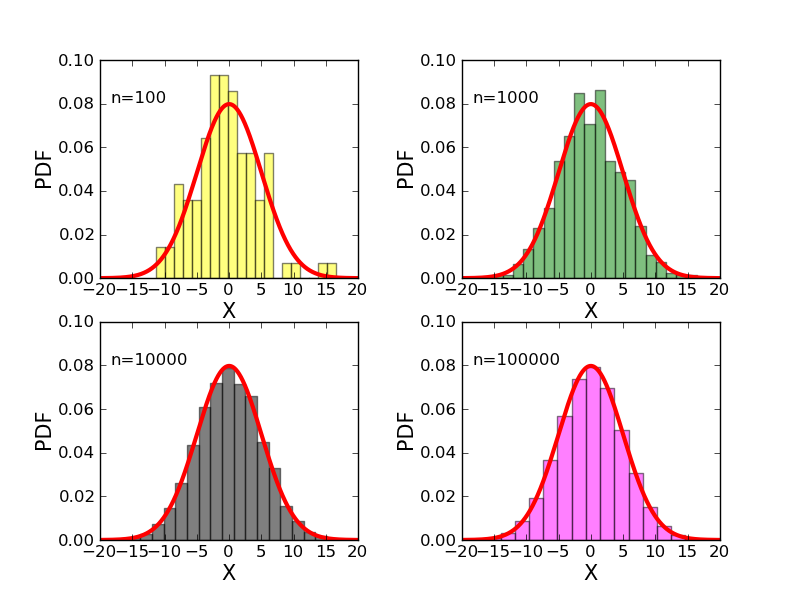
\includegraphics[width=0.5\textwidth]{images/rand_theo.png}
  \caption{Effect of the number of samples ($n$) on empirical PDF versus theoretical PDF.}
   \label{fig:pdf_norm_n}
\end{figure}
\afterfig

We can also see the effect of the number of sample on the empirical distribution apart from the normal distribution, say Laplace distribution. In this example, we are controlling the limits of the axis using the \verb"plt.xlim" and \verb"plt.ylim" separately. In case of $y-axis$ we are only defining \verb"ymax" to control the maximum limit of the axis, while for $x-axis$ we are defining both the limits. The limit of the \verb"axis" could have been fixed using the \verb"axis" as used in the last example, this is just to show that we can control only one limit, and leave the other limit to \verb"plt". Fig. \ref{fig:pdf_laplace_n} shows the empirical and theoretical pdf for various number of samples. 
\index{Distribution, Laplace}
\beforeverb \begin{verbatim}
>>> rv = st.laplace(loc=0, scale=15)
>>> x1 = np.linspace(-100, 100, 1000)
>>> y1 = rv.pdf(x1)
>>> 
>>> # compute and plot pdf
>>> plt.clf()
>>> fig = plt.figure()
>>> fig.subplots_adjust(wspace=0.4)
>>>  
>>> plt.subplot(2,2,1)
>>> x = rv.rvs(size=100)
>>> n, bins, patches = plt.hist(x, 20, normed=1, facecolor='yellow', alpha=0.5)
>>> plt.plot(x1, y1, 'r', lw=3, label='scale=5')
>>> plt.xlabel('X', fontsize=15)
>>> plt.ylabel('PDF', fontsize=15)
>>> plt.ylim(ymax=0.04)
>>> plt.xlim((-100,100))
>>> plt.text(-80,0.035,'n=100')
>>> 
>>> plt.subplot(2,2,2)
>>> x = rv.rvs(size=1000)
>>> n, bins, patches = plt.hist(x, 20, normed=1, facecolor='green', alpha=0.5)
>>> plt.plot(x1, y1, 'r', lw=3, label='scale=5')
>>> plt.xlabel('X', fontsize=15)
>>> plt.ylabel('PDF', fontsize=15)
>>> plt.ylim(ymax=0.04)
>>> plt.xlim((-100,100))
>>> plt.text(-80,0.035,'n=1000')
>>> 
>>> plt.subplot(2,2,3)
>>> x = rv.rvs(size=1000)
>>> n, bins, patches = plt.hist(x, 20, normed=1, facecolor='black', alpha=0.5)
>>> plt.plot(x1, y1, 'r', lw=3, label='scale=5')
>>> plt.xlabel('X', fontsize=15)
>>> plt.ylabel('PDF', fontsize=15)
>>> plt.ylim(ymax=0.04)
>>> plt.xlim((-100,100))
>>> plt.text(-80,0.035,'n=10000')
>>> 
>>> plt.subplot(2,2,4)
>>> x = rv.rvs(size=10000)
>>> n, bins, patches = plt.hist(x, 20, normed=1, facecolor='magenta', alpha=0.5)
>>> plt.plot(x1, y1, 'r', lw=3, label='scale=5')
>>> plt.xlabel('X', fontsize=15)
>>> plt.ylabel('PDF', fontsize=15)
>>> plt.ylim(ymax=0.04)
>>> plt.xlim((-100,100))
>>> plt.text(-80,0.035,'n=100000')
>>> 
>>> plt.savefig('/home/tomer/my_books/python_in_hydrology/laplace_rand.png')
\end{verbatim} \afterverb

\beforefig
\begin{figure}[h!]
  \centering
    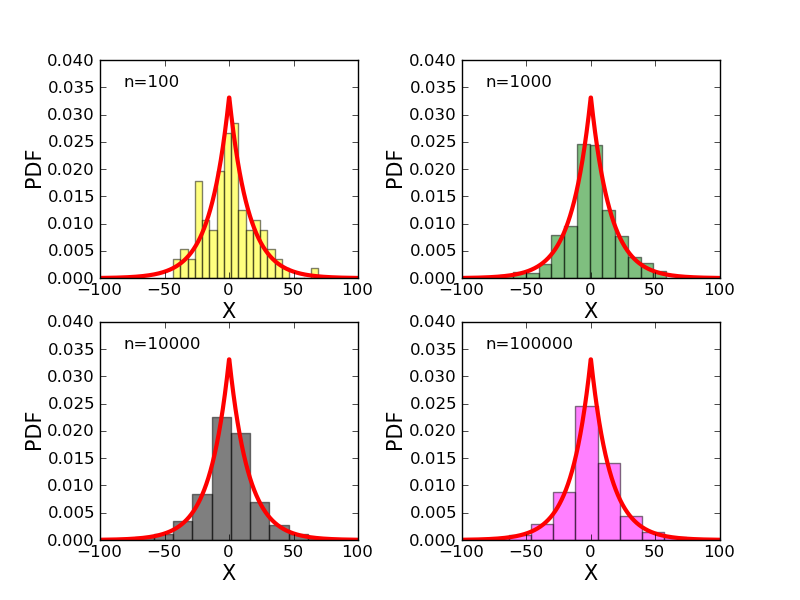
\includegraphics[width=0.5\textwidth]{images/laplace_rand.png}
  \caption{Effect of the number of samples on empirical PDF versus theoretical PDF for Laplace distribution.}
   \label{fig:pdf_laplace_n}
\end{figure}
\afterfig

\section{The t-test}
In statistics, we make hypothesis like two different random variable have the same mean, or have equal variance, or they follow same distribution. To test these hypothesis, test statistic is derived, and based on the test statistic, the hypothesis is rejected or accepted. When the test statistic follow a Student's t distribution, the t-test is used to test hypothesis. This test is available in the \verb"scipy.stats" library. Let us first test if the mean of random variable is same as we expected or not. \verb"st.ttest_1samp" function is used for this purpose. We will generate normally distributed random variable having mean equal to 5, and standard deviation equal to 10. And we will test if the mean of this generated random variable is 5 or not. Because we are talking 1000 number of sample, we expect that the mean will be approximately equal to 5 most of the time (but not always). The hypothetis is rejected or accepted based on the p-value. The p-value close to one means that hypothesis is true; a value 
closer to zero means that the hypothesis is rejected. The significance level ($\alpha$) is used to define the threshold, which is often taken as 0.05 or 0.01. If the p-value is greater than this than we can accept the hypothesis. 
\index{T-test}
\beforeverb \begin{verbatim}
>>> import scipy.stats as st
>>> rvs1 = st.norm.rvs(loc=5,scale=10,size=1000)
>>> # t-test
>>> t, p = st.ttest_1samp(rvs1,5)
>>> print(p)
0.882877605761
\end{verbatim} \afterverb
We see in this example that p-value is 0.88, which means the mean of generated random variable is close to 5. The t-test is also used to test if the mean of two independent random number is equal or not. Let us generate two normally distributed random variable with same mean, say 5. We would like to see if the mean of these two independent random variable is same or not. We can use \verb"st.ttest_ind" for this purpose. In this example the p-value is 0.96, which means means are same.
\beforeverb \begin{verbatim}
>>> rvs1 = st.norm.rvs(loc=5,scale=10,size=1000)
>>> rvs2 = st.norm.rvs(loc=5,scale=10,size=1000)
>>> # t-test
>>> t, p = st.ttest_ind(rvs1,rvs2)
>>> print(p)
0.963392592667
\end{verbatim} \afterverb

In the previous example, we tested two independent sample for the mean. We can also test if the mean is same or not, when the samples are related or come from same experiment. We can use \verb"st.ttest_rel" for this purpose. We get p-value 0.57, which means that the means are same.
\beforeverb \begin{verbatim}
>>> rvs1 = st.norm.rvs(loc=5,scale=10,size=1000)
>>> rvs2 = st.norm.rvs(loc=5,scale=10,size=1000)
>>> # t-test
>>> t, p = st.ttest_rel(rvs1,rvs2)
>>> print(p)
0.569900697821
\end{verbatim} \afterverb

\section{KS test}
\index{KS test}
Kolmogorov–Smirnov (KS) test is a non-parametric test to compare the equality of two continuous one dimensional probability distributions. In this test, we quantify the distance (absolute difference) between distributions. These two distributions could be two different sample, or one could be sample and another one a theoretical distribution. Let us test if our generated normal random variable follow normal distribution or not. \verb"st.kstest" is the function to to perform KS test. 
\beforeverb \begin{verbatim}
>>> import numpy as np
>>> import scipy.stats as st
>>> x = np.random.randn(1000) 
>>> # KS test
>>> D, p = st.kstest(x,'norm')
>>> print(p)
0.652473310995
\end{verbatim} \afterverb
We get a p-value equal to 0.65, which means that our generated normally distributed random variable is in fact normal. We can also test if the the generated uniformly distributed random variable are not normal by chance. In this we get a p-value equal to 0, which means that our generated random numbers in this case are not normal. 
\beforeverb \begin{verbatim}
>>> y = np.random.rand(1000) 
>>> D, p = st.kstest(y,'norm')
>>> print(p)
0.0
\end{verbatim} \afterverb

\section{The chi square test}
\index{Chi square test}
We can also compare distribution by comparing their PDFs. In this case we use the Chi square ($\chi^2$) test. In this test, $\chi^2$ statistics is computed first, and based on this we say if distributions are same or not. We can compare sample with the theoretical distribution, or two samples. We will take two pdfs, in which one is assumed to be observed and another one is expected. We will use the \verb"chisquare" function from \verb"scipy.stats.mstats" library. This function gives  $\chi^2$ statistics and p-value of the test. In the following example, we get a p-value close to zero, it means that these two frequency comes from different distributions.
\beforeverb \begin{verbatim}
>>> from scipy.stats.mstats import chisquare
>>> import numpy as np
>>> f_obs = np.array([10, 15, 20, 30]) # observed pdf
>>> f_exp = np.array([10, 5, 15, 30]) # expected pdf
>>> # chi square test
>>> c, p = chisquare(f_obs, f_exp)
>>> 
>>> print(c,p)
(21.666666666666668, 7.6522740548062336e-05)
\end{verbatim} \afterverb

\section{Measure of statistical dependence}
\index{Pearson's correlation}
\index{Spearman's correlation}
\index{Kandall's tau}

Often we are interested in knowing if two hydrological variables are dependant or not. In this section, it will be described to check their statistical dependency. If two variable are statistically dependent, it does not mean that they are physically also dependent. First we will generate two variables having different relationship between them. Few with perfect relationship, and few with some noise added. In the following example, we are creating six variables: 
\begin{itemize}
\item Perfect linear relationship ($y = a +bx$),
\item Linear relationship with some noise ($y = a +bx + \epsilon $),
\item Quadratic relationship which is monotonic ($y = x^2 $),
\item Quadratic relationship with some noise ($y = x^2 + \epsilon $),
\item Quadratic relationship but this one is not monotonic ($y = (x-5)^2 $), and
\item Noise added to previous one ($y = (x-5)^2 + \epsilon $).
\end{itemize}
Fig. \ref{fig:corr} shows these variables. Out of the six variable, three have perfect relationship, and three has some noise. We would expect our measure of statistical dependence to reveal this. 
\beforeverb \begin{verbatim}
>>> import numpy as np
>>> import matplotlib.pyplot as plt
>>> 
>>> x = np.linspace(0,10)
>>> y1 = 2*x 
>>> y2 = y1 + 2*np.random.randn(50)
>>> y3 = x**2
>>> y4 = y3 + 2*np.random.randn(50)
>>> y5 = (x-5)**2
>>> y6 = y5 + 2*np.random.randn(50)
>>> 
>>> plt.subplot(2,3,1)
>>> plt.plot(x, y1, '.')
>>> plt.text(2,15,'(a)')
>>> 
>>> plt.subplot(2,3,2)
>>> plt.plot(x, y2, '.')
>>> plt.text(2,15,'(b)')
>>> 
>>> plt.subplot(2,3,3)
>>> plt.plot(x, y3, '.')
>>> plt.text(2,80,'(c)')
>>> 
>>> plt.subplot(2,3,4)
>>> plt.plot(x, y4, '.')
>>> plt.text(2,100,'(d)')
>>> 
>>> plt.subplot(2,3,5)
>>> plt.plot(x, y5, '.')
>>> plt.text(2,20,'(e)')
>>> 
>>> plt.subplot(2,3,6)
>>> plt.plot(x, y6, '.')
>>> plt.text(2,25,'(f)')
>>> plt.savefig('/home/tomer/my_books/python_in_hydrology/images/corr.png')
\end{verbatim} \afterverb

\beforefig
\begin{figure}[h!]
  \centering
    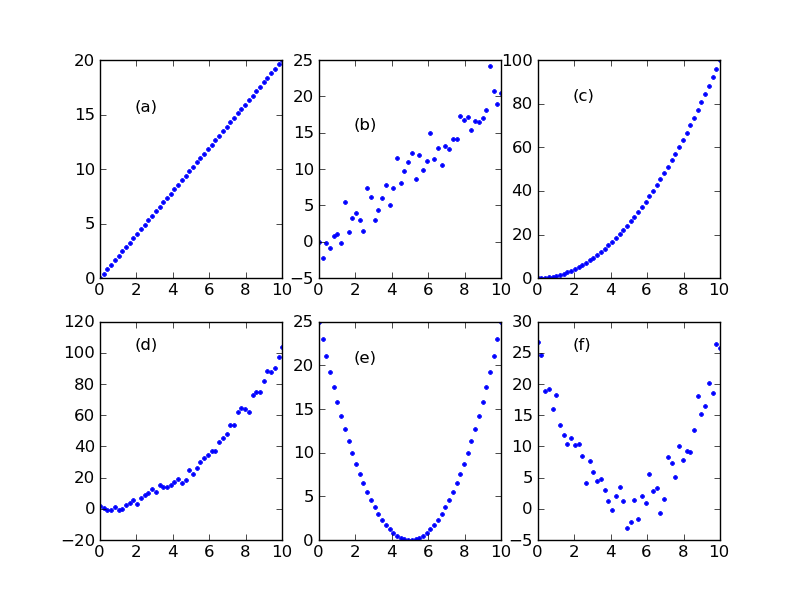
\includegraphics[width=0.5\textwidth]{images/corr.png}
  \caption{Different kind of relationship between two variables.}
   \label{fig:corr}
\end{figure}
\afterfig

Unfortunately there is no measure to reveal the strength of relationship in case on non-linearty.  The reason for this is that we can have any form of non linear relationship which is not possible for measure to quantity. Having said that, there are some measure which work well in some case. We will explore few of them. First begin with Pearson's correlation coefficient, which provides the strength of linear relationship. \verb"st.pearsonr" function can be used to compute Pearson's correlation coefficient. This function also gives the p-value, which can be used to quantity the significance of the relationship. We are using \verb"%" 
operator for formatting the output. \verb".2f" tells to print the output till second decimal places. 
\beforeverb \begin{verbatim}
>>> import scipy.stats as st
>>> r1, p1 = st.pearsonr(x,y1)
>>> r2, p2 = st.pearsonr(x,y2)
>>> r3, p3 = st.pearsonr(x,y3)
>>> r4, p4 = st.pearsonr(x,y4)
>>> r5, p5 = st.pearsonr(x,y5)
>>> r6, p6 = st.pearsonr(x,y6)
>>> 
>>> # print r's
>>> print('%.2f %.2f %.2f %.2f %.2f %.2f')%(r1,r2,r3,r4,r5,r6)
1.00 0.97 0.97 0.96 0.00 -0.02
\end{verbatim} \afterverb
We get 1.0 for first case, and a value slightly lesser than 1.0 for second case, because we perturbed the relationship. In third case, we get a value of 0.97, while in reality the relationship is perfect though not linear. The value is 0 in fifth case, even though the relationship perfect. So we can conclude that Pearson's correlation coefficient is good {\bf only} to measure the linear relationship. Now we will compute Spearman's correlation coefficient for all these six cases using \verb"st.spearman".
\beforeverb \begin{verbatim}
>>> rho1, p1 = st.spearmanr(x,y1)
>>> rho2, p2 = st.spearmanr(x,y2)
>>> rho3, p3 = st.spearmanr(x,y3)
>>> rho4, p4 = st.spearmanr(x,y4)
>>> rho5, p5 = st.spearmanr(x,y5)
>>> rho6, p6 = st.spearmanr(x,y6)
>>> 
>>> # print rho's
>>> print('%.2f %.2f %.2f %.2f %.2f %.2f')%(rho1,rho2,rho3,rho4,rho5,rho6)
1.00 0.97 1.00 0.99 0.01 -0.04
\end{verbatim} \afterverb
Spearman's correlation coefficient is providing the similar output like one by Spearman's except that it is able to recognize the relationship in third and fourth case better. In the third and fourth case, the relationship was non-linear but monotonic. Spearman's correlation coefficient is useful measure when the data has monotonic behaviour. But this is also not working properly in case when the relationship is well defined, but not monotonic. Kendall's tau correlation coefficient is a statistics to measure the rank correlation. Kendall's tau can be computed using the \verb"st.kendalltau" function. 
\beforeverb \begin{verbatim}
>>> tau1, p1 = st.kendalltau(x,y1)
>>> tau2, p2 = st.kendalltau(x,y2)
>>> tau3, p3 = st.kendalltau(x,y3)
>>> tau4, p4 = st.kendalltau(x,y4)
>>> tau5, p5 = st.kendalltau(x,y5)
>>> tau6, p6 = st.kendalltau(x,y6)
>>> 
>>> # print tau's
>>> print('%.2f %.2f %.2f %.2f %.2f %.2f')%(tau1,tau2,tau3,tau4,tau5,tau6)
1.00 0.86 1.00 0.95 0.01 -0.05
\end{verbatim} \afterverb
This provides measure similar to that of Spearman's correlation coefficient, and is unable to reveal non-monotonic relationship that we have in fifth and sixth case. 

\section{Linear regression}
\index{Linear regression}
Linear regression is an approach to model the relationship between two variables using linear function. We will use \verb"st.linregress" function to perform linear regression. We will first generate some synthetic data using a known linear model,
and will also add some noise using normally distributed random variable. \verb"linregress" provides correlation, p-value, and standard error of estimate apart from model coefficients.  

\beforeverb \begin{verbatim}
>>> import numpy as np
>>> import scipy.stats as st
>>> # generate the data
>>> n = 100 # length of the data
>>> x = np.random.rand(n)
>>> y = 3 + 7*x + np.random.randn(n)
>>> # perform linear regression
>>> b, a, r, p, e = st.linregress(x, y)
>>> print(a,b)
(2.9059642495310403, 7.3015273619236618)
\end{verbatim} \afterverb

We generated data using linear model ($y=3+7x+\epsilon$), while linear regression ($y=2.91+7.3x$). The difference in the fitted model and true model, is because of the noise. As you add more noise, you will see that the fitted model departs more from the reality. Fig. \ref{fig:line} shows the true line ($y=3+7x$), corrupted measurement ($y=3+7x+\epsilon$), fitted line ($y=2.91+7.3x$), and prediction interval for the fitted line. The fitted line and true line are matching reasonably. The prediction interval are also quiet reasonable. \\

The variance of a predicted $Y_{pred}$ is given by,
\begin{equation}
\sigma^2_{pred} = E[(Y_{pred} - \widehat{Y})^2] = \sigma^2_\epsilon \left( 1 + \frac{1}{n} +  \frac{(X_0 - \overline{X})^2}{\sum_{i=1}^n (X-\overline{X})^2}\right).
\end{equation}

Where, the $\sigma^2_\epsilon$ is estimated by $s^2$ the classic unbiased estimator of the residual variance. The  $\sigma^2_{pred}$  is used to generate prediction interval using a Students $t$ distribution with $n - 2$ degrees of freedom (because $s^2$ is an estimator). The confidence interval around $Y_{pred}$ is given by,
\begin{equation}
\label{eq:pi}
PI  = \sigma_{pred} *z
\end{equation}
where, $PI$ is the prediction interval, $z$ is the value of Students $t$ distribution at $\alpha$ significance level. 

\beforeverb \begin{verbatim}
>>> eps = y - a - b*x  # error of fitting and measured data
>>> x1 = np.linspace(0, 1) # x axis to plot the PI
>>> # variace of fitting error
>>> e_pi = np.var(eps)*(1+1.0/n + (x1-x.mean())**2/np.sum((x-x.mean())**2))
>>> # z value using the t distribution and with dof = n-2
>>> z = st.t.ppf(0.95, n-2)
>>> # prediction interval
>>> pi = np.sqrt(e_pi)*z
>>> zl = st.t.ppf(0.10, n-2) # z at 0.1
>>> zu = st.t.ppf(0.90, n-2) # z at 0.9
>>> ll = a + b*x1 + np.sqrt(e_pi)*zl # 10 %
>>> ul = a + b*x1 + np.sqrt(e_pi)*zu # 90 %
\end{verbatim} \afterverb

Finally, we can plot the true line, fitted line, measurement corrupted with noise and prediction intervals. 
\beforeverb \begin{verbatim}
>>> import matplotlib.pyplot as plt
>>> plt.plot(x,y,'ro', label='measured')
>>> plt.plot(x1,ll,'--', label='10%')
>>> plt.plot(x1,ul,'--', label='90%')
>>> plt.xlabel('x')
>>> plt.ylabel('y')
>>> plt.legend(loc='best')
>>> plt.savefig('/home/tomer/my_books/python_in_hydrology/images/lin_regress.png')
\end{verbatim} \afterverb

\beforefig
\begin{figure}[h!]
  \centering
    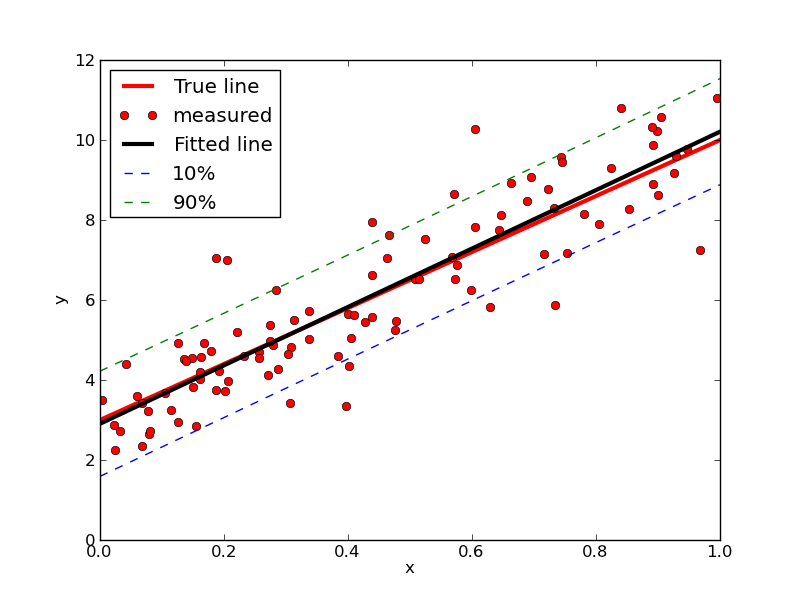
\includegraphics[width=0.5\textwidth]{images/lin_regress.png}
  \caption{The fitted line along with the uncertainty intervals.}
   \label{fig:line}
\end{figure}
\afterfig

\section{Polynomial regression}
\index{Non-linear regression}
We can do the polynomial regression using the \verb"np.polyfit". This provides the fitted coefficients. We can define the order of polynomial as third argument to the \verb"np.polyfit" function. First, we are generating a second degree polynomial ($y=1+2x-3x^2$),
then we are adding noise into it. 
\beforeverb \begin{verbatim}
>>> import numpy as np
>>> # generate data
>>> x = np.linspace(0,10)
>>> y = 1 + 2*x - 3*x**2 + 15*np.random.randn(50)
>>> # fit the polynomial
>>> z = np.polyfit(x,y,2)
>>> print(z)
[-3.03571947  1.34263078  4.58790632]
\end{verbatim} \afterverb
The \verb"np.polyfit" function is providing fitted polynomial as $y=4.58+1.34x-3.03x^2$, while the coefficient of true polynomials were different. Only the third parameter is computed reasonably. Other two parameters differs a lot compared to the true one. Let us look into the behaviour of fitted polynomials compared to the true polynomial. \verb"np.poly1d" function is used to evaluate the polynomial using the fitted coefficient returned by \verb"np.polyfit". Fig. \ref{fig:curve} shows the resulted plot. Though the fitted coefficients differed than real coefficients, but the fitted polynomial is quiet close to the true one. The parameter associated with second degree was computed quiet reasonably by the \verb"np.polyfit", this means that this is the most sensitive parameters compared to other one.

\beforeverb \begin{verbatim}
>>> import matplotlib.pyplot as plt
>>> # evaluate polynomial 
>>> p = np.poly1d(z)
>>> z_true = np.array([-3, 2, 1]) # coefficient of true polynomial
>>> p_true = np.poly1d(z_true) # true polynomial
>>> # plot
>>> plt.plot(x, y,'.r', label='noisy data')
>>> plt.plot(x, p_true(x), label='True curve')
>>> plt.plot(x, p(x), label='Fitted curve')
>>> plt.xlabel('x')
>>> plt.ylabel('y')
>>> plt.legend()
>>> plt.savefig('/home/tomer/my_books/python_in_hydrology/images/cuve_regre.png')
\end{verbatim} \afterverb

\beforefig
\begin{figure}[h!]
  \centering
    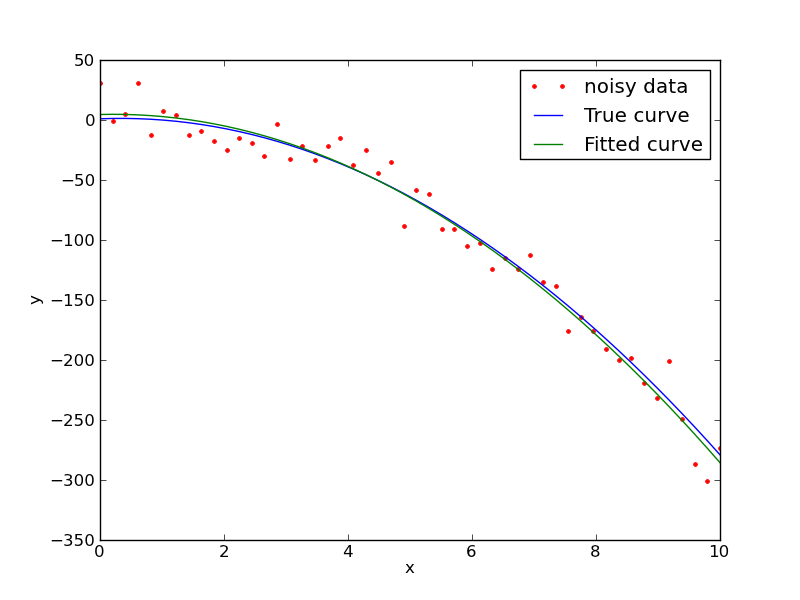
\includegraphics[width=0.5\textwidth]{images/curve_regre.png}
  \caption{Fitted curve along with true curve, and data with noise.}
   \label{fig:curve}
\end{figure}
\afterfig

\section{Interpolation}
\index{Interpolation}
There are various way of doing interpolation. Commonly used methods are piecewise linear and non-linear, splines, and radial basis functions. In this section, we will use piecewise linear and radial basis function to interpolate the data.\\

 We will first generate few data points having exponential relationship. Then we will interpolate using \verb"interp1d" function of \verb"scipy.interpolate" library. This function returns an object, which can be used later to evaluate the fitted piecewise linear curve at required data points. Fig. \ref{fig:interp1d} shows the fitted piecewise polynomial along with the data used to generate it.
\beforeverb \begin{verbatim}
>>> import matplotlib.pyplot as plt
>>> import numpy as np
>>> from scipy.interpolate import interp1d
>>> # generate data
>>> x = np.linspace(0,1,5)
>>> y = np.exp(-x)
>>> f = interp1d(x, y)
>>> xnew = np.linspace(x.min(), x.max())
>>> ynew = f(xnew)   # use interpolation function returned by `interp1d`
>>> # plot
>>> plt.plot(x, y, 'ro', label='y')
>>> plt.plot(xnew, ynew, '-', label='ynew')
>>> plt.xlabel('x')
>>> plt.ylabel('y')
>>> plt.legend()
>>> plt.savefig('/home/tomer/my_books/python_in_hydrology/images/inter.png')
\end{verbatim} \afterverb

\beforefig
\begin{figure}[h!]
  \centering
    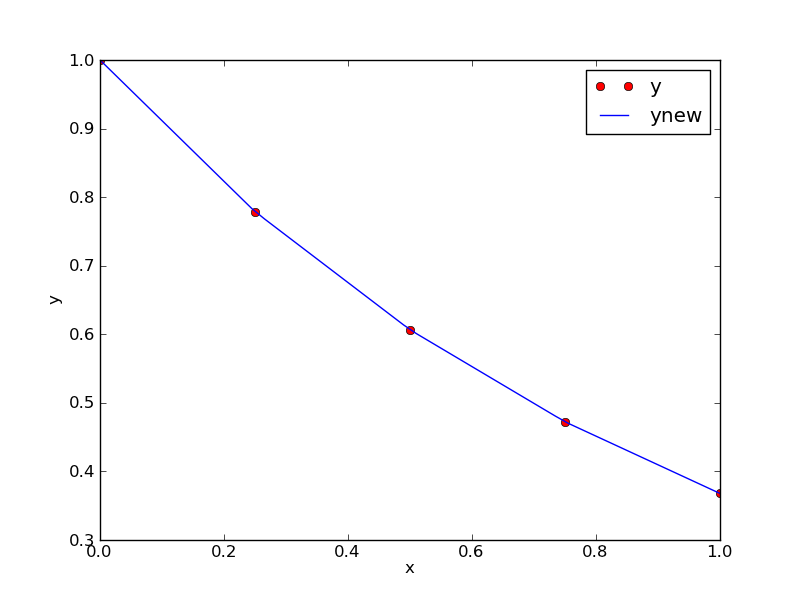
\includegraphics[width=0.5\textwidth]{images/inter.png}
  \caption{Interpolated curve versus the measured data.}
   \label{fig:interp1d}
\end{figure}
\afterfig

The \verb"inerp1d" does not do extrapolation i.e. it will issue an error if we want to fit the data outside input data range. We can suppress the error by specifying the \verb"bounds_error=None" argument. In this case, it will give \verb"nan", if we want to interpolate outside input data range. To interpolate outside the input data range, we can use \verb"Rbf" function of the \verb"scipy.interpolate" library. Remember in section 4.4, the interpolated data was only in the range of location of input data. We will use \verb"Rbf" function to interpolate outside these range. We are using \verb"plt.imshow" to make the 2D plot. Fig. \ref{fig:rbf} shows the plot. IT is clear from the figure, that it is able to interpolate outside input data range also. 
\beforeverb \begin{verbatim}
>>> x = np.random.rand(5)
>>> y = np.random.rand(5)
>>> pet = 2+2*np.random.rand(5)
>>> 
>>> rbfi = sp.interpolate.Rbf(x, y, pet)  # radial basis function interpolation instance
>>> 
>>> xi = np.linspace(0,1)
>>> yi = np.linspace(0,1)
>>> XI, YI = np.meshgrid(xi,yi)  # gridded locations
>>> 
>>> di = rbfi(XI, YI)   # interpolated values
>>> 
>>> plt.imshow(di, extent=(0,1,0,1), origin='lower')
>>> plt.scatter(x,y, color='k')
>>> plt.xlabel('X')
>>> plt.ylabel('Y')
>>> plt.axis((0,1,0,1))
>>> plt.savefig('/home/tomer/my_books/python_in_hydrology/images/rbf.png')
\end{verbatim} \afterverb

\beforefig
\begin{figure}[h!]
  \centering
    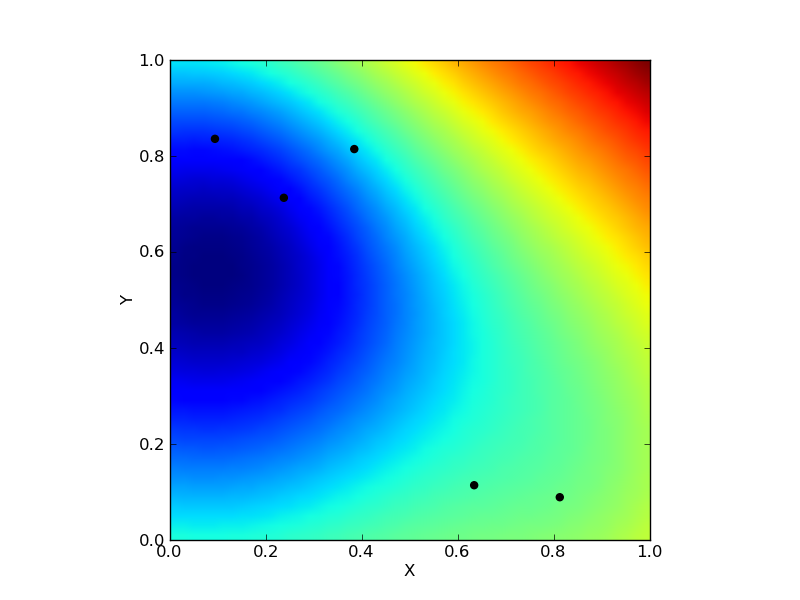
\includegraphics[width=0.5\textwidth]{images/rbf.png}
  \caption{Interpolation in 2D.}
   \label{fig:rbf}
\end{figure}
\afterfig

\section{Autocorrelation}
\index{Autocorrelation}
Autocorrelation is the correlation of a signal with itself. This tells the how a signal is related in time or space. This can be used to see the periodicity in the signal. To demonstrate this, we will first generate a signal using sine with a periodicity of $4\pi$ and magnitude of 2. Fig. \ref{fig:corr_0} shows the signal in upper panel, and autocorrelation in lower panel. The autocorrelation is plotted using the \verb"plt.acorr" function. We have shown the grid in the plot using the \verb"plt.grid" function. The horizontal lines at 0 and $e^{-1}$ are plotted using the \verb"plt.axhline". Autocorrelation is showing a nice periodic behaviour with a periodicity of $4\pi$.

\beforeverb \begin{verbatim}
>>> import numpy as np
>>> import matplotlib.pyplot as plt
>>> x = 2*np.sin(np.arange(100)/2.0) # periodic signal
>>> x += np.random.randn(len(x)) # corrupted with noise
>>> 
>>> plt.subplot(2,1,1)
>>> plt.plot(x, '-s')
>>> plt.ylabel('x', fontsize=20)
>>> plt.grid(True)
>>> plt.xlabel('Time')
>>> 
>>> plt.subplot(2,1,2)
>>> c = plt.acorr(x, usevlines=True, normed=True, maxlags=50, lw=2)
>>> plt.grid(True)
>>> plt.axhline(0, color='black', lw=2)
>>> plt.axhline(1/np.exp(1), color='red')
>>> plt.ylabel('Autocorrelation')
>>> plt.xlim(xmin=0,xmax=100)
>>> plt.xlabel('Lag')
>>> plt.savefig('/home/tomer/my_books/python_in_hydrology/images/corr_0.png')
\end{verbatim} \afterverb

\beforefig
\begin{figure}[h!]
  \centering
    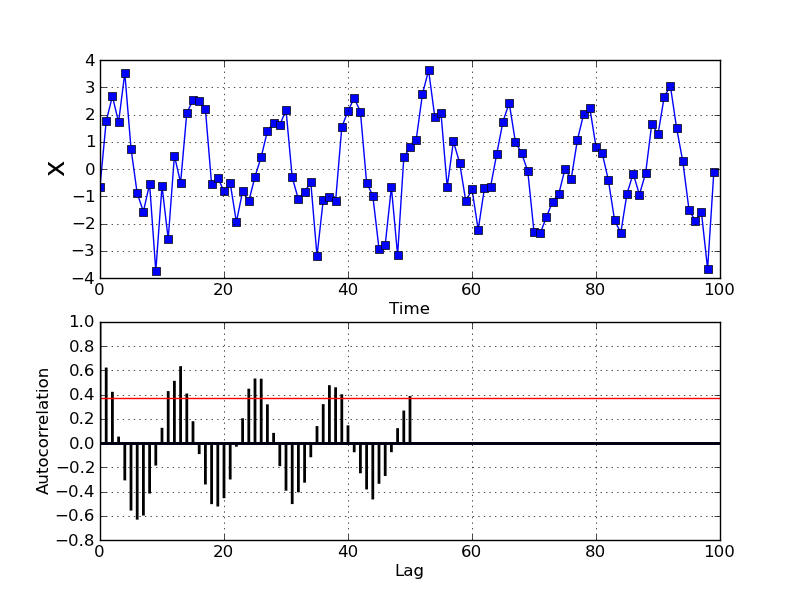
\includegraphics[width=0.5\textwidth]{images/corr_0.png}
  \caption{A plot showing 100 random numbers generated using sine function, and an autocorrelation of the series.}
   \label{fig:corr_0}
\end{figure}
\afterfig

Autocorrelation function is also used to compute the correlation length. Correlation length is the distance from a point beyond which
there is no further correlation of a physical property associated with that point. Mathematically, the correlation length is the lag at which autocorrelation is equal to $e^{-1}$, which is shown by a horizontal red line in the plot. Let us make a plot with higher periodicity to compute correlation length. The resulted plot is shown in Fig. \ref{fig:corr_1}. Graphically we see that correlation is approximately 9. 

\beforeverb \begin{verbatim}
>>> import numpy as np
>>> import matplotlib.pyplot as plt
>>> x = 2*np.sin(np.arange(100)/10.0) # periodic signal
>>> x += np.random.randn(len(x)) # corrupted with noise
>>> 
>>> plt.subplot(2,1,1)
>>> plt.plot(x, '-s')
>>> plt.ylabel('x', fontsize=20)
>>> plt.grid(True)
>>> plt.xlabel('Time')
>>> 
>>> plt.subplot(2,1,2)
>>> c = plt.acorr(x, usevlines=True, normed=True, maxlags=50, lw=2)
>>> plt.grid(True)
>>> plt.axhline(0, color='black', lw=2)
>>> plt.axhline(1/np.exp(1), color='red')
>>> plt.ylabel('Autocorrelation')
>>> plt.xlim(xmin=0,xmax=100)
>>> plt.xlabel('Lag')
>>> plt.savefig('/home/tomer/my_books/python_in_hydrology/images/corr_1.png')
\end{verbatim} \afterverb

\beforefig
\begin{figure}[h!]
  \centering
    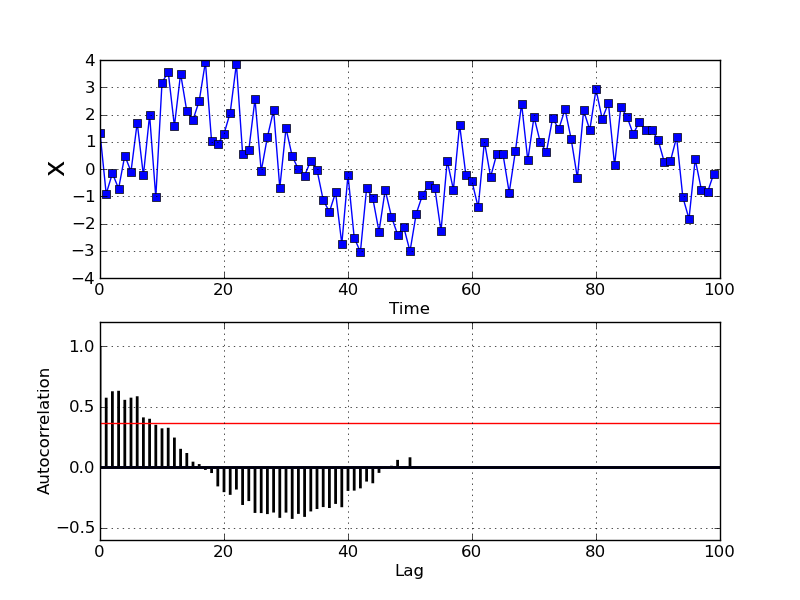
\includegraphics[width=0.5\textwidth]{images/corr_1.png}
  \caption{A plot showing 100 random numbers generated using sine function, and an autocorrelation of the series.}
   \label{fig:corr_1}
\end{figure}
\afterfig

To precisely determine the correlation length, we would be fitting a interpolation function between lag and correlation length, and then determine the lag where autocorrelation becomes $e^{-1}$. The \verb"plt.acorr" function return lags and autocorrelation at these lags. First we will assign lags and correlation to separate variables. We also print the lags to see what is inside it.

\beforeverb \begin{verbatim}
>>> lags = c[0] # lags
>>> auto_corr = c[1] # autocorrelation
>>> print(auto_corr)
[-50 -49 -48 -47 -46 -45 -44 -43 -42 -41 -40 -39 -38 -37 -36 -35 -34 -33
 -32 -31 -30 -29 -28 -27 -26 -25 -24 -23 -22 -21 -20 -19 -18 -17 -16 -15
 -14 -13 -12 -11 -10  -9  -8  -7  -6  -5  -4  -3  -2  -1   0   1   2   3
   4   5   6   7   8   9  10  11  12  13  14  15  16  17  18  19  20  21
  22  23  24  25  26  27  28  29  30  31  32  33  34  35  36  37  38  39
  40  41  42  43  44  45  46  47  48  49  50]
\end{verbatim} \afterverb

The \verb"acorr" provides positive and negative lags. We don't need both, we can get rid of it by giving a index which is in boolean format and is obtained by using the statement \verb"lags>=0". We also remove the autocorrelation array which corresponds to negative lags. 
\beforeverb \begin{verbatim}
>>> auto_corr = auto_corr[lags>=0]
>>> lags = lags[lags>=0]
\end{verbatim} \afterverb
Now, we need the autocorrelation at two point, one just above the threshold, and one just below the threshold. We get their indices by counting how many times the auto correlation is above threshold. 
\beforeverb \begin{verbatim}
>>> n = sum(auto_corr>np.exp(-1))
>>> print(n)
9
\end{verbatim} \afterverb
One point is at 8th indices, and another is at 9th indices. Now, we can use \verb"interp1d" to get the value of exact lag when autocorrelation is equal to threshold. This provides the correlation length which is 8.65.
\beforeverb \begin{verbatim}
>>> f = interp1d([auto_corr[n], auto_corr[n-1]], [lags[n], lags[n-1]])
>>> corr_len = f(np.exp(-1))
array(8.64725236367028)
\end{verbatim} \afterverb

\section{Uncertainty Intervals}
Many times, we get a number of ensembles of the data. And we want to see the behaviour of these ensemble. Let us first begin by generating ensemble, and then plotting them. In this example, first we are generating a signal with sin behaviour. Then, we are using \verb"vstack" to stack the data i.e. to make 2 dimensional array using many one dimensional arrays. After this, we mix some noise in the data so that ensemble looks slightly different. We are transposing the data using \verb"T" attributes for plotting, otherwise it will plot ensemble on $x-axis$ instead of time. 
\beforeverb \begin{verbatim}
>>> import numpy as np
>>> import matplotlib.pyplot as plt
>>> import scipy.stats as st
>>> 
>>> # generate some data
>>> x = 100*np.sin(np.linspace(0,10,100))
>>> X = np.vstack([x,x,x,x,x,x,x,x,x,x,x,x,x,x,x,x,x,x,x,x])
>>> e = 10*np.random.randn(20,100) 
>>> 
>>> X_err = X+e
>>> 
>>> plt.plot(X_err.T, 'k')
>>> plt.xlabel('Time')
>>> plt.ylabel('X')
>>> plt.savefig('/home/tomer/my_books/python_in_hydrology/images/X_err.png')
\end{verbatim} \afterverb

\beforefig
\begin{figure}[h!]
  \centering
    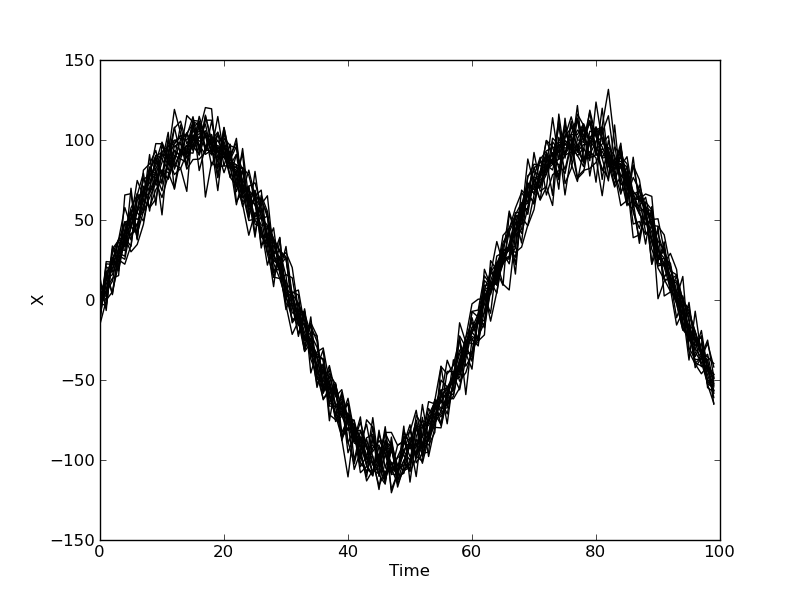
\includegraphics[width=0.5\textwidth]{images/X_err.png}
  \caption{Various ensemble of data.}
   \label{fig:X_err}
\end{figure}
\afterfig

Fig. \ref{fig:X_err} shows the plot of these ensembles. We see that all the ensemble are behaving similar to each one. But we can not infer anything more on the behaviour of ensemble using this plot. A better way to visualize ensemble is by using the various uncertainty intervals along with the mean. We can compute the uncertainty interval at various percentile using the \verb"st.scoreatpercentile" function. We are computing 10$^th$, 50$^th$, and 90$^th$ percentile. 50$^th$ percentile is the median. We are plotting median than the mean, because if there are some outliers in the data, median provided better insight into the behaviour of ensemble. Fig. \ref{fig:X_uncern} shows the median,  10$^th$, and 90$^th$ of ensemble. Using this plot, we can make out that the spreads of the ensemble is not same everywhere; it is relatively more in the peak and valley and less elsewhere.

\beforeverb \begin{verbatim}
>>> ll = st.scoreatpercentile(X_err, 10) # 10th percentile
>>> ml = st.scoreatpercentile(X_err, 50) # 50th percentile
>>> ul = st.scoreatpercentile(X_err, 90) # 90th percentile
>>> 
>>> plt.plot(ml, 'g', lw=2, label='Median')
>>> plt.plot(ul, '--m', label='90%')
>>> plt.plot(ll, '--b', label='10%')
>>> plt.xlabel('Time')
>>> plt.ylabel('X')
>>> plt.legend(loc='best')
>>> plt.savefig('/home/tomer/my_books/python_in_hydrology/images/X_uncer.png')
\end{verbatim} \afterverb

\beforefig
\begin{figure}[h!]
  \centering
    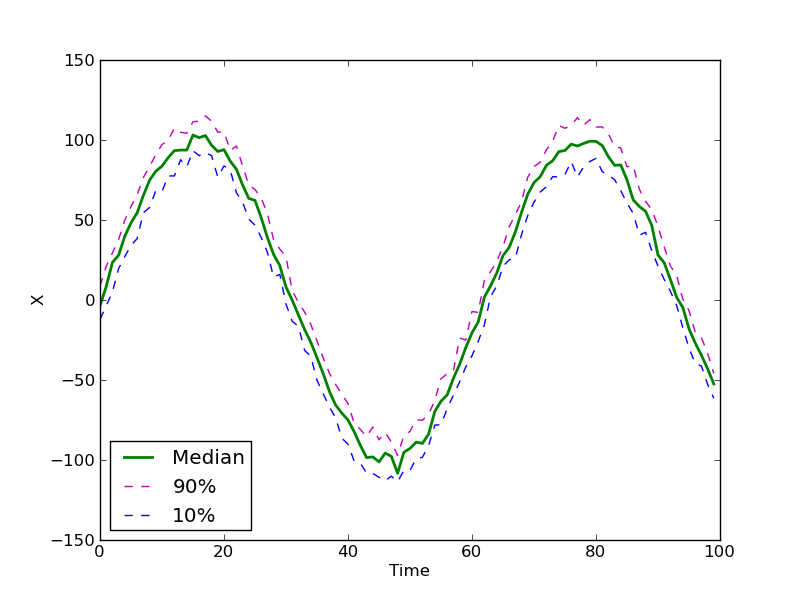
\includegraphics[width=0.5\textwidth]{images/X_uncer.png}
  \caption{The median, and uncertainty intervals of data estimated from ensemble.}
   \label{fig:X_uncern}
\end{figure}
\afterfig

The uncertainty intervals could be plotted by shaded regions. The \verb"plt.fill_between" provides the option of filling color in between two array, and can be used to make a shaded regions.

\beforeverb \begin{verbatim}
>>> plt.plot(ml, 'g', lw=2, label='Median')
>>> plt.fill_between(range(100), ul, ll, color='k', alpha=0.4, label='90%')
>>> plt.xlabel('Time')
>>> plt.ylabel('X')
>>> plt.legend(loc='best')
>>> plt.savefig('/home/tomer/my_books/python_in_hydrology/images/X_uncer_shade.png')
\end{verbatim} \afterverb
Fig. \ref{fig:X_uncern_shaded} shows the plot of uncertainty using the shaded region.

\beforefig
\begin{figure}[h!]
  \centering
    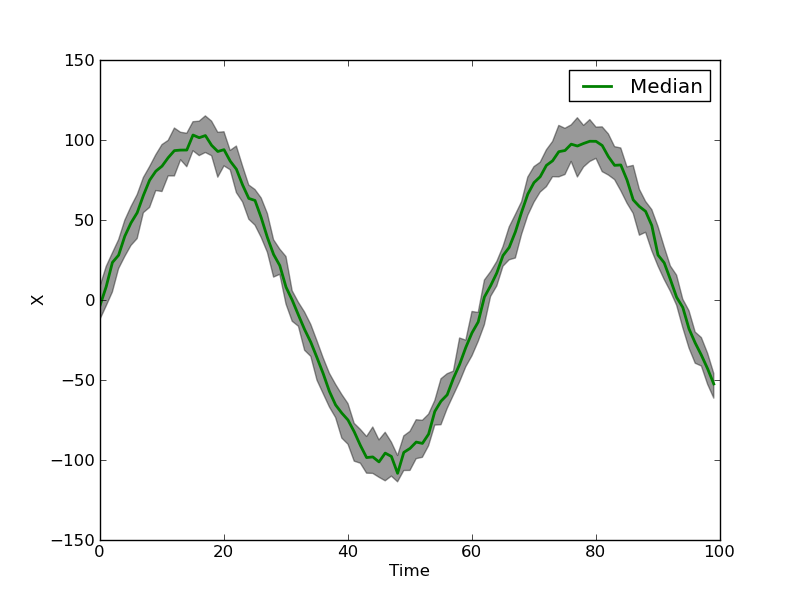
\includegraphics[width=0.5\textwidth]{images/X_uncer_shade.png}
  \caption{The median, and uncertainty intervals of data estimated from ensemble. The uncertainty intervals are shown using shaded region.}
   \label{fig:X_uncern_shaded}
\end{figure}
\afterfig

\chapter{Spatial Data}
\section{Types of spatial data}
\index{Raster}
\index{Vector}
Raster and vector are the two basic data structures for storing and manipulating images and graphics data in GIS (Geographic Information Systems). Raster image comes in the form of individual pixels, and each spatial location or resolution element has a pixel associated where the pixel value indicates the attribute, such as color, elevation, or an ID number. Vector data comes in the form of points and lines, that are geometrically and mathematically associated. Points are stored using the coordinates, for example, a two-dimensional point is stored as (x, y). Lines are stored as a series of point pairs, where each pair represents a straight line segment, for example, (x1, y1) and (x2, y2) indicating a line from (x1, y1) to (x2, y2).\\

We will create some raster data using some mathematical function, and then also add noise into it. We will keep both the data (with noise, and without noise) for future use. \verb"np.mgrid" is used to create gridded points. The data is plotted using \verb"plt.matshow" function, which is a simple function to visualize a two dimensional array. Fig. \ref{fig:spatial_data} shows the data without noise, data corrupted with noise is shown in Fig. \ref{fig:spatial_data_noisy}. The data without noise shows a systematic behaviour, while it is blurred in the data added with noise.

\beforeverb \begin{verbatim}
>>> import numpy as np
>>> # generate some synthetic data
>>> X, Y = np.mgrid[0:101, 0:101]
>>> data = np.sin((X**2 + Y**2)/25) 
>>> data_noisy = data + np.random.random(X.shape)
>>>    
>>> # plot the data
>>> plt.matshow(data)
>>> plt.colorbar()
>>> plt.savefig('/home/tomer/my_books/python_in_hydrology/images/spatial_data.png')
>>> 
>>> plt.matshow(data_noisy)
>>> plt.colorbar(shrink=0.5)
>>> plt.savefig('/home/tomer/my_books/python_in_hydrology/images/spatial_data_noisy.png')
\end{verbatim} \afterverb

\beforefig
\begin{figure}[h!]
  \centering
    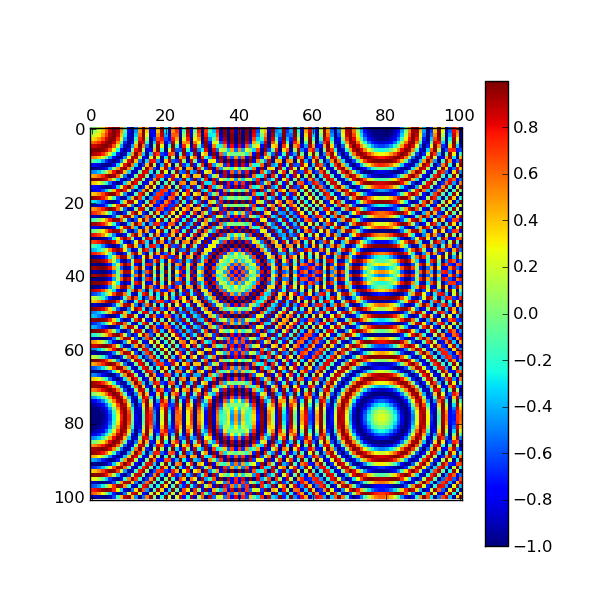
\includegraphics[width=0.5\textwidth]{images/spatial_data.png}
  \caption{Synthetic data created.}
   \label{fig:spatial_data}
\end{figure}
\afterfig

\beforefig
\begin{figure}[h!]
  \centering
    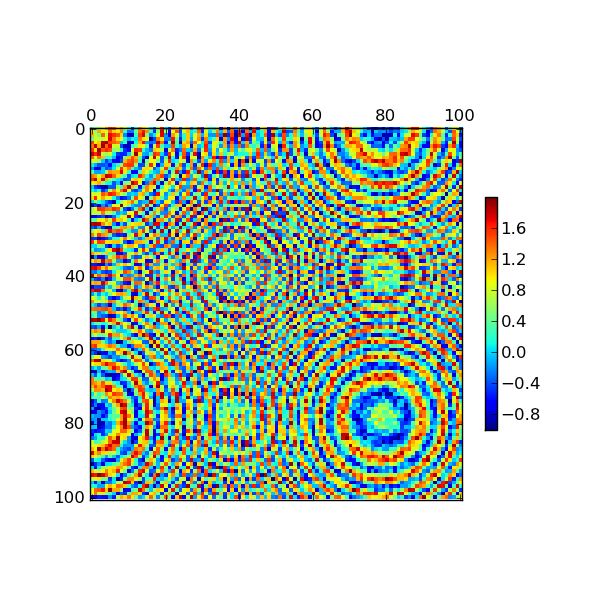
\includegraphics[width=0.5\textwidth]{images/spatial_data_noisy.png}
  \caption{Synthetic data perturbed with noise.}
   \label{fig:spatial_data_noisy}
\end{figure}
\afterfig

We can also generate a vector data with using some points. Fig. \ref{fig:vect} shows the vector data. 

\beforeverb \begin{verbatim}
>>> # vector data
>>> vector_x = [10,7,24,16,15,10]
>>> vector_y = [10,23,20,14,7,10]
>>> 
>>> #plot vector data
>>> plt.clf()
>>> plt.plot(vector_x, vector_y)
>>> plt.axis((5,25,5,25))
>>> plt.savefig('/home/tomer/my_books/python_in_hydrology/images/vect.png')
\end{verbatim} \afterverb

\beforefig
\begin{figure}[h!]
  \centering
    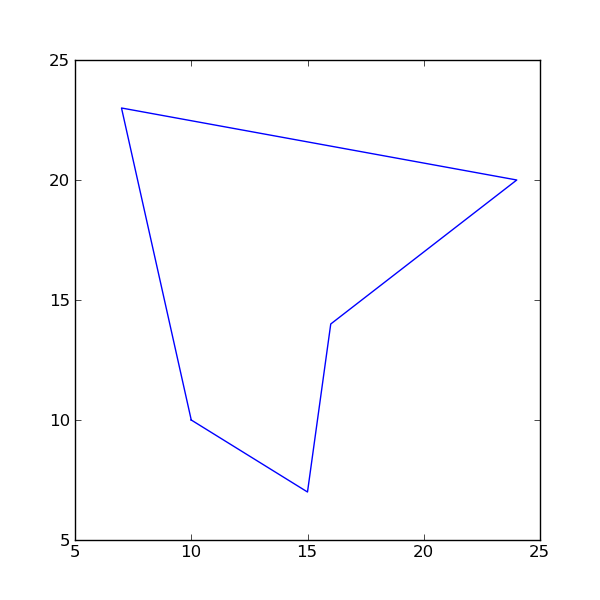
\includegraphics[width=0.5\textwidth]{images/vect.png}
  \caption{Vector data.}
   \label{fig:vect}
\end{figure}
\afterfig

The geospatial data can be classified into two major parts. In the first part we have information about some feature, like a two dimensional array showing the spatial variation in elevation etc. In the second part, we have information about the co-ordinates of the data. A typical processing chain for geo-spatial data is given in flow chart \ref{fig:flowchart_geo}. We have the geospatial data, and we extract the feature information and co-ordinate information separately, then we process them separately, and finally after processing we again combine them. The processing for feature information could be some mathematical operation, and for co-ordinate information, it could some co-ordinate transformation etc.

% styles for flowcharts
\tikzstyle{decision} = [diamond, draw, text width=3cm, text badly centered, node distance=3cm, inner sep=0pt]
\tikzstyle{block} = [rectangle, draw, text width=3cm, text centered, rounded corners, minimum height=2em]
\begin{figure}[h]
 \begin{center}
  \begin{tikzpicture}[node distance=3cm, auto, >=stealth]
   % nodes
   \node[block] (a)  				                    {Geospatial data};
   \node[]      (b)  [below of=a, node distance=2cm]                       {};
   \node[block] (c)  [right of=b]                       {Co-ordinate information};
   \node[block] (d)  [left of=b, node distance=2cm]  	{Feature information};
   \node[block] (e)  [below of=d, node distance=2cm]  	{Processing};
   \node[block] (f)  [below of=c, node distance=2cm]  	{Processing};
   \node[block] (g)  [below of=a, node distance=6cm]   {Processed geospatial data};
      
   % edges
   \draw[->] (a) -- (c);
   \draw[->] (a) -- (d);
   \draw[->] (d) -- (e);
   \draw[->] (c) -- (f);
   \draw[->] (e) -- (g);
   \draw[->] (f) -- (g);
   \end{tikzpicture}
  \caption{Flowchart showing a typical chain for processing the geospatial data.}
  \label{fig:flowchart_geo}
 \end{center}
\end{figure}

\section{Geoinformation}
\index{Geotransform}
The raster data can be geo-referenced  either by specifying the \verb"GeoTransform" variable, or by specifying the GCPs for the image. The GeoTransform ($GT$) is related to the geographical co-ordinates in the following way,
\begin{eqnarray}
X_{geo} = GT[0] + X_{image}*GT[1] + Y_{image}*GT[2], \\
Y_{geo} = GT[3] + X_{image}*GT[4] + Y_{image}*GT[5],
\end{eqnarray}
where, subscript $geo$ refers to the global co-ordinates, and $image$ refers to the image co-ordinates, i.e. pixel and line number of image. The number in the square bracket ($[]$) represents the indices of the $GT$ variables. $X$ and $Y$ are co-ordinates. $GT[2]$ and $GT[4]$ represents the orientation of the image, with respect to the $X$ and $Y$ of $geo$, and becomes zero if the image is north up. $GT[1]$ represents pixel width, and $GT[5]$ represents the pixel height. $GT[0]$ and $GT[3]$ is the position of the  top left corner of the top left pixel of the raster. It should be noted that the pixel/line coordinates in the above are from (0.0,0.0) at the top left corner of the top left pixel to at the bottom right corner of the bottom right pixel. The pixel/line location of the center of the top left pixel would therefore be (0.5,0.5).\\

The information related to the geo-referencing can be specified by specifying the control points. Control points should contains minimally the $GCP_{Pixel}$ (pixel number of image), $GCP_{Line}$ (line number of image), $GCP_X$ (X co-ordinate), $GCP_Y$ (Y co-ordinate), and $GCP_Z$ (Z co-ordinate). The (Pixel,Line) position is the GCP location on the raster. The (X,Y,Z) position is the associated georeferenced location with the Z often being zero. Usually polynomials are used to transform the image co-ordinate (Pixel,Line) into geo-referenced co-ordinates. \\

Normally a dataset will contain either an affine geotransform or GCPs. In addition to the information about how co-ordinates are related to the geo-referenced co-ordinates, the name of co-ordinate system is also assigned to the image. 

\section{Writing Raster}
\index{Gtiff}
\index{Raster, write}
There are various format for storing the raster data; Geotiff is the most commonly used. We will use \verb"gdal" library to read and write the raster data. Check if you have installed \verb"gdal" by issuing the command \verb"import gdal". If you get no error, then things are under control, otherwise go to \url{http://trac.osgeo.org/gdal/wiki/DownloadSource}, download and install the latest version. Let us first write the the data in GeoTIFF format. First we will write the data without noise.
\beforeverb \begin{verbatim}
>>> import gdal
>>> driver = gdal.GetDriverByName('GTiff')
>>> file_name = "/home/tomer/my_books/python_in_hydrology/datas/data.tif"
>>> dataset = driver.Create(file_name, data.shape[1], data.shape[0], 1, 
... gdal.GDT_Float32)
>>> dataset.SetGeoTransform((664000.0, 100.0, 0.0, 1309000.0, 0.0, -100.0))
>>> dataset.GetRasterBand(1).WriteArray(data, 0, 0)
>>> dataset = None
\end{verbatim} \afterverb

First we created the driver, and asked it to create GTIFF file. Other types of format can also be created. A list of the format supported by gdal, and their code for creating the driver are listed at \url{http://www.gdal.org/formats_list.html}, e.g. code for portable network graphics is PNG. Then we create the database i.e. we create the file in computer, by issuing command \verb"dirver.Create". The inputs required to \verb"Create" are name of the file, size of the data, number of band in the data, format of the data. Then we define the geoinformation by issuing the \verb"SetGeoTransform" command. And finally we write the data using the method \verb"GetRasterBand". It is good practice to close the data with defining the dataset as \verb"None". If path for the specified file name does not exist, it returns None, and will give error if other operations are performed over it. \\

In the similar way, we can write the data corrupted with noise. 

\beforeverb \begin{verbatim}
>>> driver = gdal.GetDriverByName('GTiff')
>>> file_name = "/home/tomer/my_books/python_in_hydrology/datas/data_noisy.tif"
>>> dataset = driver.Create(file_name, data_noisy.shape[1], data_noisy.shape[0], 1, gdal.GDT_Float32)
>>> dataset.SetGeoTransform((664000.0, 100.0, 0.0, 1309000.0, 0.0, -100.0))
>>> dataset.GetRasterBand(1).WriteArray(data_noisy, 0, 0)
>>> dataset = None
\end{verbatim} \afterverb


\section{Writing Vector}
\index{Shapefile}
\index{Vector, write}
Shapefile (.shp) format is quiet commonly used type of vector data. Let us write one shapefile. To write shapefile, we will be using the package \verb"ogr". OGR is a part of the GDAL library. OGR deals with the vector formats, while GDAL main library is for raster formats. A list of format supported by OGR along with their code name to be used while creating driver, is given at \url{http://www.gdal.org/ogr/ogr_formats.html}. Let us say, we want to make a shapefile having location of the four cities  and their name. The details of cities are as:

\begin{tabular}{lll}
Name 		& Latitude 	& Longitude \\
Bijnor		& 29.4 		& 78.1 \\
Delhi		& 28.6		& 77.2 \\
Bangalore	& 13.0		& 77.8 \\
Berambadi	& 11.8		& 76.6 \\
\end{tabular}

We begin with importing \verb"ogr" library and defining the location and names of the cities. 
\beforeverb \begin{verbatim}
>>> import ogr
>>> lat = [29.4,28.6,13.0,11.8]
>>> lon = [78.1,77.2,77.8,76.6]
>>> name = ['Bijnor', 'Delhi', 'Bangalore', 'Berambadi']
\end{verbatim} \afterverb

Now, we define the name of driver (ESRI Shapefile), and create the data source. \verb"driver.CrateDataSource" defines the name of the folder where data will be saved. \verb"ds.CreateLayer" defines the name of the shapefile along with the geometry type (point in this case). Then we define, field name as 'Name' and say that it is a string type having a maximum width of 16. 

\beforeverb \begin{verbatim}
>>> driver = ogr.GetDriverByName("ESRI Shapefile")
>>> ds = driver.CreateDataSource('/home/tomer/my_books/python_in_hydrology/datas/')
>>> layer = ds.CreateLayer('location', geom_type=ogr.wkbPoint)
>>> field_defn = ogr.FieldDefn('Name', ogr.OFTString )
>>> field_defn.SetWidth(16)
>>> layer.CreateField(field_defn)
\end{verbatim} \afterverb

Now, we have the basic information ready, and we can start adding the information about cities (name and location). First we create a feature to store the information about city. Then, we add the name of the city in the 'Name' field. After this, we say that it is point type, and we add its longitude and latitude. At last, we destroy the feature and data source, so that nothing else can be done with them, and our data is saved properly. 
\beforeverb \begin{verbatim}
>>> i = 0
>>> for i in range(len(name)):
>>>     feature = ogr.Feature(layer.GetLayerDefn())
>>>     feature.SetField('Name', name[i])
>>>     pt = ogr.Geometry(ogr.wkbPoint)
>>>     pt.SetPoint_2D(0, lon[i], lat[i])
>>>     feature.SetGeometry(pt)
>>>     layer.CreateFeature(feature)
>>>     feature.Destroy()
>>> ds.Destroy()
\end{verbatim} \afterverb

We can see this shapefile in any GIS viewere. Fig. \ref{fig:location} shows the location of cities which was generated using QGIS. 

\beforefig
\begin{figure}[h!]
  \centering
    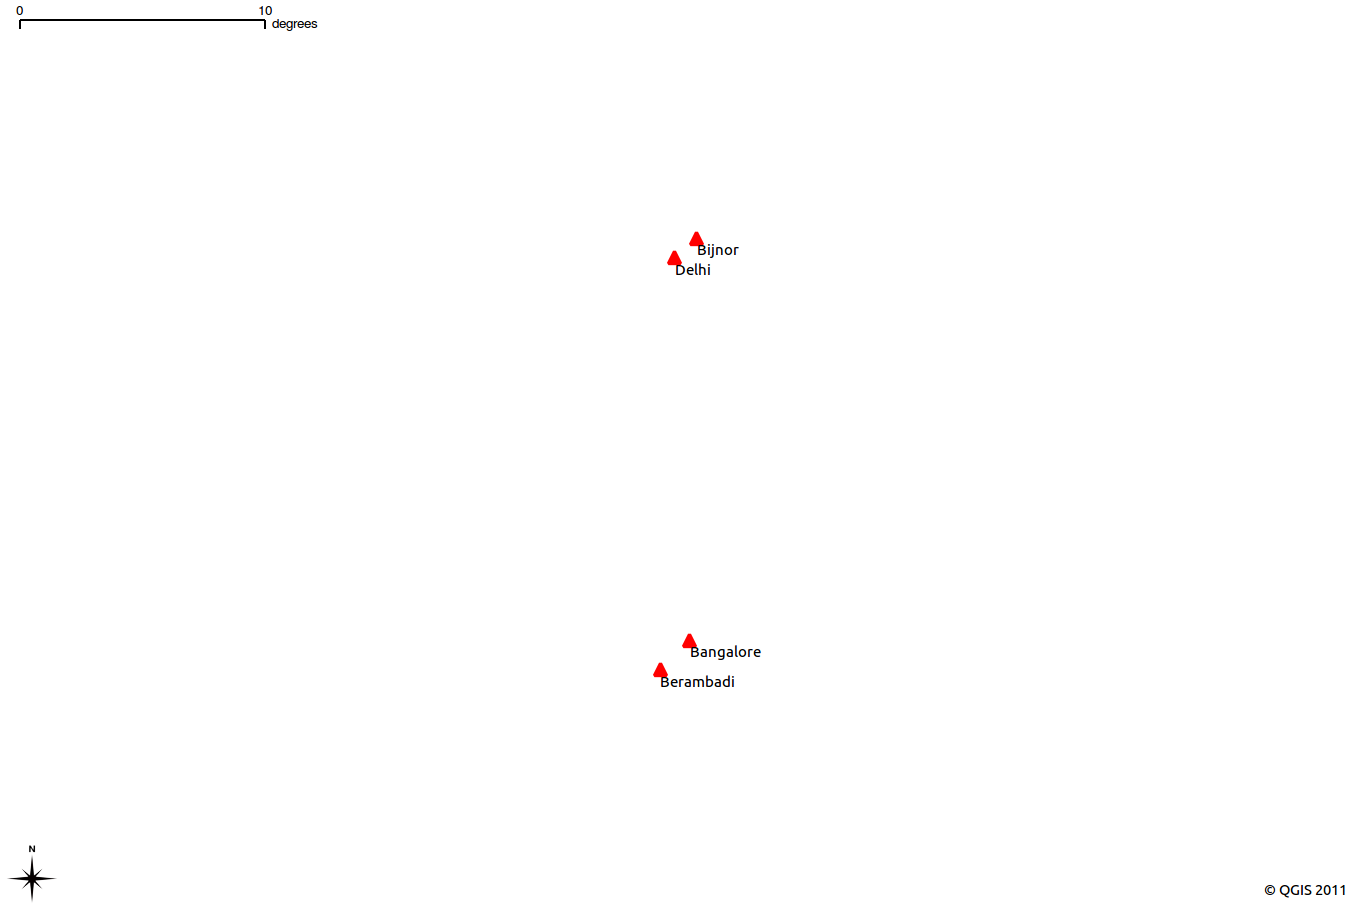
\includegraphics[width=1.0\textwidth]{images/location.png}
  \caption{Location of the cities.}
   \label{fig:location}
\end{figure}
\afterfig

\section{Reading the raster}
\index{Raster, read}
In this section, we will read the data that we wrote in earlier section. We will read the raster data that has noise in it. 
\beforeverb \begin{verbatim}
>>> driver = gdal.GetDriverByName('GTiff')
>>> file_name = "/home/tomer/my_books/python_in_hydrology/datas/data_noisy.tif"
>>> dataset = gdal.Open(file_name, GA_ReadOnly)
>>> geotransform = dataset.GetGeoTransform()
>>> data = dataset.GetRasterBand(1).ReadAsArray()
>>> dataset = None
\end{verbatim} \afterverb

\section{Read the vector}
\index{Vector, read}
In this section, we will read the vector data, that we wrote earlier. First, we need to import \verb"ogr" library. Then we open data source by specifying the directory of the shapefile. Then, we use \verb"GetLayerByName" to read the shapefile by specifying the name of shpaefile without .shp extension. After this, we are printing \verb"\n" which means print a blank line. \verb"\n" represents a new line, and \verb"\t" represents the tab. Now, we are printing header information (SI., Name, Latitude, Longitude). We are using \verb".format" to format the output. The number inside \verb" '{}' " after the colon (:) represents the length of the output. The we read the feature in the shapefile one by one using the \verb"for" loop. From each feature, we extract the name using \verb"GetFieldAsString", Longitude using \verb"GetX" and  Latitude using \verb"GetY". At the end to avoid corrupting the database, we close it safely by specifying data source as \verb"None".
\index{ogr}

\beforeverb
\begin{verbatim}
>>> import ogr
>>> ds = ogr.Open( '/home/tomer/my_books/python_in_hydrology/datas/' )
>>> lyr = ds.GetLayerByName('location' )
>>> 
>>> print("\n")
>>> print("{} \t {:10s} \t {} \t {}".format('SI', 'Name', 'Longitude', 'Latitude'))
>>> for feat in lyr:
>>>     geom = feat.GetGeometryRef()
>>>     name = feat.GetFieldAsString(0)
>>>     lat = geom.GetX()
>>>     lon = geom.GetY()
>>>     print('{0} \t {1:10s} \t {2:.3f} \t \t {3:.3f}'.format(0, name, lat, lon ))
>>>    
>>> ds = None

SI 	Name       	 Latitude 	 Longitude
0 	 Bijnor     	 78.100 	 	 29.400
0 	 Delhi      	 77.200 	 	 28.600
0 	 Bangalore  	 77.800 	 	 13.000
0 	 Berambadi  	 76.600 	 	 11.800
\end{verbatim}
\afterverb

\section{Filtering}
\index{Filtering}
The active RADAR data is affected by speckle/noise. Before we extract some useful information from the satellite data, we need to remove/minimize these speckle from the data. These filters essentially try to remove the high frequency information. In reality this high frequency information need not to be noise. So we need to specify how much filtering we want. The types of filter can be divided into two categories: adaptive and non adaptive filters. Adaptive filters adapt their weightings across the image to the speckle level, and non-adaptive filters apply the same weightings uniformly across the entire image. In this section, we will be using one example of both category. We will use median filter from the non-adaptive filter category, and Wiener filter from the adaptive category. \\

We can import the \verb"medfilt2d" function from the \verb"scipy.signal" library. First, we read the noisy data that we saved in tif format from hard disk. Then we apply a filter to it having window size of $3\times3$. Fig. \ref{fig:median} shows the filtered image. When, we compare this image with the original image, and with the image in which we mixed some noise, we see that filtered images showed more smooth variation, but is not showing no where near to the original image. 
\index{Filter, Median}
\beforeverb \begin{verbatim}
>>> from osgeo import gdal
>>> from scipy.signal import medfilt2d
>>> from osgeo.gdalconst import *
>>> import matplotlib.pyplot as plt
>>> 
>>> # read the raster data 
>>> driver = gdal.GetDriverByName('GTiff')
>>> file_name = "/home/tomer/my_books/python_in_hydrology/datas/data_noisy.tif"
>>> dataset = gdal.Open(file_name, GA_ReadOnly)
>>> geotransform = dataset.GetGeoTransform()
>>> data = dataset.GetRasterBand(1).ReadAsArray()
>>> dataset = None
>>> 
>>> data_median = medfilt2d(data, kernel_size=3) # median filter of 3X3 window
>>> # plot the data
>>> plt.matshow(data_median)
>>> plt.colorbar()
>>> plt.savefig('/home/tomer/my_books/python_in_hydrology/images/median.png')
\end{verbatim} \afterverb

\beforefig
\begin{figure}[h!]
  \centering
    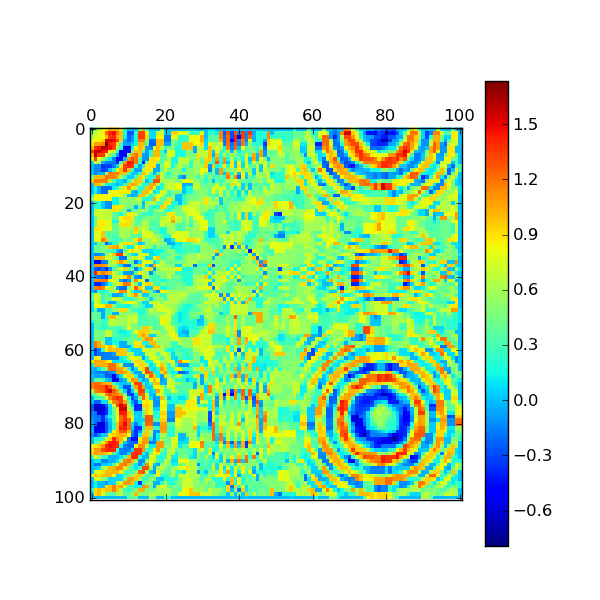
\includegraphics[width=0.5\textwidth]{images/median.png}
  \caption{Noisy data after filtering with median filter.}
   \label{fig:median}
\end{figure}
\afterfig
\index{Filter, Wiener}
Now, we apply Wiener filter on the same dataset. We keep the same window size for Wiener filter also. After doing the filtering, we are also saving the data in tif format. This tell use, how can read some geospatial data, process the feature information (matrix in this case), and then save the feature information with the co-ordinate information. 
\beforeverb \begin{verbatim}
>>> from scipy.signal import wiener
>>> data_wiener = wiener(data, mysize=(3,3)) # Wiener filter 
>>> # plot
>>> plt.matshow(data_wiener)
>>> plt.colorbar()
>>> plt.savefig('/home/tomer/my_books/python_in_hydrology/images/wiener.png')
>>> 
>>> # save the data into tif format
>>> driver = gdal.GetDriverByName('GTiff')
>>> file_name = "/home/tomer/my_books/python_in_hydrology/datas/data_filtered.tif"
>>> dataset = driver.Create(file_name, data_wiener.shape[1], data_wiener.shape[0], 1, gdal.GDT_Float32)
>>> dataset.SetGeoTransform(geotransform)
>>> dataset.GetRasterBand(1).WriteArray(data_wiener, 0, 0)
>>> dataset = None
\end{verbatim} \afterverb

\beforefig
\begin{figure}[h!]
  \centering
    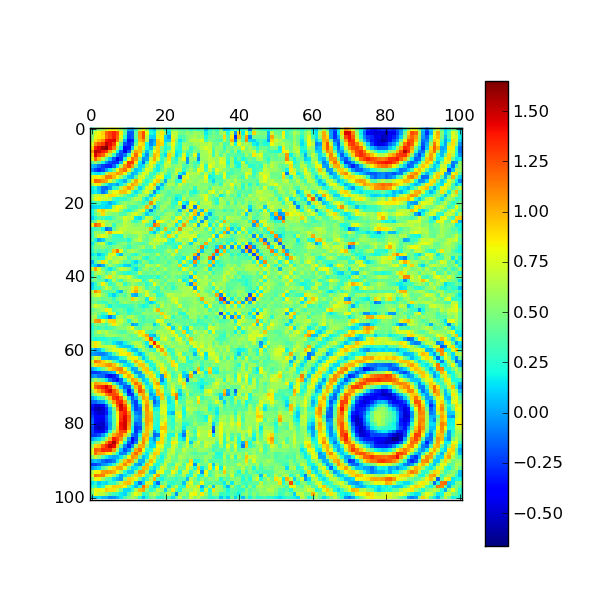
\includegraphics[width=0.5\textwidth]{images/wiener.png}
  \caption{Noisy data after filtering with Wiener filtering.}
   \label{fig:wiener}
\end{figure}
\afterfig

\section{NDVI}
Normalized Difference Vegetation Index (NDVI) is a index to analyse variation in the vegetation. The formula to compute NDVI is as:
\begin{equation}
NDVI = \frac{NIR-RED}{NIR+RED}
\end{equation}
\index{NDVI}

We begin with importing libraries, and do not forget to import \verb"division" from \verb"__future__" library. This is to avoid the integer division. Then we read the data that is in tiff format. To compute NDVI, we need data for NIR (band4) and RED (band3). 
\beforeverb \begin{verbatim}
>>> # import the required library
>>> from __future__ import division
>>> from osgeo import gdal
>>> from osgeo.gdalconst import *
>>> import matplotlib.pyplot as plt
>>> 
>>> # read the banda 3 raster data 
>>> driver = gdal.GetDriverByName('GTiff')
>>> file_name = "/home/tomer/my_books/python_in_hydrology/datas/band3.tif"
>>> dataset = gdal.Open(file_name, GA_ReadOnly)
>>> geotransform = dataset.GetGeoTransform()
>>> projection = dataset.GetProjection()
>>> band3 = dataset.GetRasterBand(1).ReadAsArray()
>>> dataset = None
>>> # read the band 4 raster data
>>> file_name = "/home/tomer/my_books/python_in_hydrology/datas/band4.tif"
>>> dataset = gdal.Open(file_name, GA_ReadOnly)
>>> band4 = dataset.GetRasterBand(1).ReadAsArray()
>>> dataset = None
\end{verbatim} \afterverb

Apart from the data, we are also retrieving the \verb"geotransform" and \verb"projection" information. Let us print them one by one. 
\beforeverb \begin{verbatim}
>>> print(geotransform)
(76.5, 0.001, 0.0, 11.85, 0.0, -0.001)
\end{verbatim} \afterverb
The first entry in this tell us, that latitude and longitude for the north-west corner are 11.85 and 76.5 respectively. Resolution of data is 0.001 in both x and y direction, and the image has no rotation. Let us print now, projection information. 
\beforeverb \begin{verbatim}
>>> print(projection)
GEOGCS["WGS 84",DATUM["unknown",SPHEROID["WGS84",6378137,298.257223563]],
PRIMEM["Greenwich",0],UNIT["degree",0.0174532925199433]]
\end{verbatim} \afterverb
This tells us that the datum of data is WGS84, and our data is in geographic co-ordinates (latitude and longitude). More details on the projections and their parameters can be found at \url{http://spatialreference.org}. \\

We can check the data type using \verb"dtype" attributes. We see that data type integer. That is why we have imported \verb"division" from \verb"__future__" library, to avoid integer division. 
\beforeverb \begin{verbatim}
>>> print(band3.dtype)
uint8
\end{verbatim} \afterverb 

Now we compute NDVI, and plot the result using \verb"matshow". In \verb"matshow", we are also specifying \verb"vmin" and \verb"vmax" to control the extent of \verb"colorbar". 
\beforeverb \begin{verbatim}
>>> ndvi = (band4-band3)/(band4+band3)
>>> 
>>> plt.matshow(ndvi,cmap=plt.cm.jet, vmin=-1, vmax=1)
>>> plt.colorbar(shrink=0.8)
>>> plt.savefig('/home/tomer/my_books/python_in_hydrology/images/ndvi.png')
\end{verbatim} \afterverb

\beforefig
\begin{figure}[h!]
  \centering
    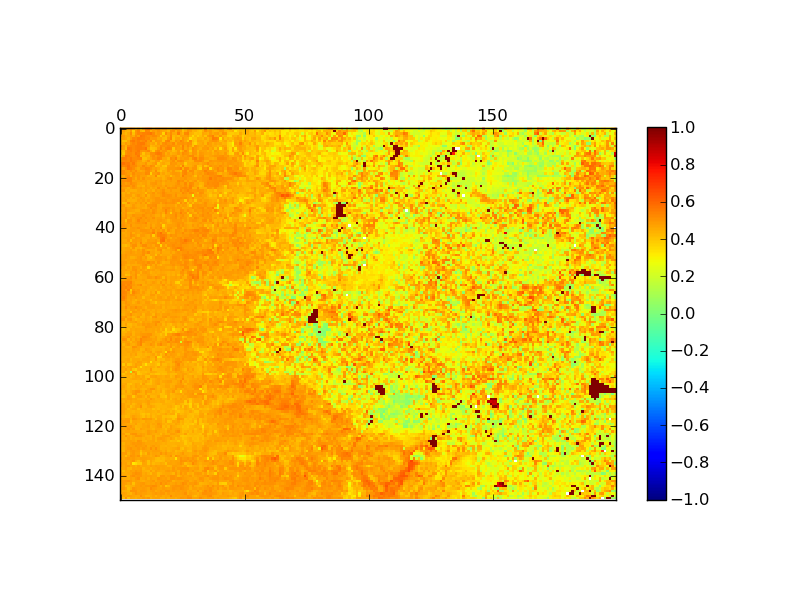
\includegraphics[width=0.5\textwidth]{images/ndvi.png}
  \caption{Normalized difference vegetation index.}
   \label{fig:ndvi}
\end{figure}
\afterfig


\section{Calling GDAL as External Command}}
GDAL library provides many useful programs e.g. modifying the coordinate system, resolution and extent of the GIS data, and many more. A complete list of these can be found at \url{http://www.gdal.org/gdal_utilities.html}. In this section we will change the resolution, extent and co-ordinate system of the data. Unfortunately, Python bindings are not available for these programs, so we can not use them as we were using other Python programs. These GDAL's program works in command line mode, and Python provides a way to run external command from the Python. So, we will use this to make use of the power of the GDAL library. Before jumping into the GDAL, we will very briefly see how to run external command from Python. On Linux, we get the list of file in a directory by using the command \verb"ls" and the \verb"ls -al" provides the details of these files/directory also.
\beforeverb \begin{verbatim}
>>> from subprocess import call
>>> dir_list = call(["ls", "-l"])
>>> print(dir_list)
-rw-rw-r-- 1 tomer tomer   990 2011-12-21 17:31 auto_corr.py
-rw-rw-r-- 1 tomer tomer   199 2012-01-20 18:38 call_external.py
\end{verbatim} \afterverb
Notice that we are giving the argument to the command as a separate member of the list. This can become confusing as the number of arguments increases. On the linux shell we would have simply written \verb"ls -al", why cant we do in the same way here? Lets try to write it like this.
\beforeverb \begin{verbatim}
>>> dir_list = call("ls -al")
Traceback (most recent call last):
  File "<stdin>", line 1, in <module>
  File "/usr/lib/python2.7/dist-packages/spyderlib/widgets/externalshell/startup.py", line 122, in runfile
    execfile(filename, glbs)
  File "/home/tomer/svn/python-in-hydrology/codes/call_external.py", line 11, in <module>
    dir_list = call(["ls -al"])
  File "/usr/lib/python2.7/subprocess.py", line 493, in call
    return Popen(*popenargs, **kwargs).wait()
  File "/usr/lib/python2.7/subprocess.py", line 679, in __init__
    errread, errwrite)
  File "/usr/lib/python2.7/subprocess.py", line 1239, in _execute_child
    raise child_exception
OSError: [Errno 2] No such file or directory
\end{verbatim} \afterverb
Python gives the error in this way. To do so we should tell Python that take the input as we do int Shell, which is done by providing argument \verb"shell = True". Look at the following example.
\beforeverb \begin{verbatim}
>>> dir_list = call("ls -al", shell=True)
>>> print(dir_list)
-rw-rw-r-- 1 tomer tomer   990 2011-12-21 17:31 auto_corr.py
-rw-rw-r-- 1 tomer tomer   199 2012-01-20 18:38 call_external.py
\end{verbatim} \afterverb
This gives the desired output. This is sufficient to know about \verb"subprocess" module to work with external commands when you need to call GDAL as an external commands. 


Let us first change the projection of the data to UTM, then select a subwindow from this image, and finally change the resolution of the data. Let us first see how to do this in command line mode. It is always a good practice to first try your command in shell before using this from within the Python script. We will use the ASTER DEM to work with. The ASTER data is provided in geographical coordinates. I will be using the \verb"ASTGTM_N11E076.tif" image, which is the DEM for the Kabini river basin, South India. The path to this file in my computer is \verb"/home/tomer/berambadi/DEM/ASTGTM_N11E076_dem.tif", replace it with path of your file. First we will see the information of this tif file.
\beforeverb \begin{verbatim}
$ gdalinfo /home/tomer/berambadi/DEM/ASTGTM_N11E076_dem.tif
Warning 1: TIFFReadDirectoryCheckOrder:Invalid TIFF directory; tags are not sorted in ascending order
Driver: GTiff/GeoTIFF
Files: /home/tomer/berambadi/DEM/ASTGTM_N11E076_dem.tif
Size is 3601, 3601
Coordinate System is:
GEOGCS["WGS 84",
    DATUM["WGS_1984",
        SPHEROID["WGS 84",6378137,298.257223563,
            AUTHORITY["EPSG","7030"]],
        AUTHORITY["EPSG","6326"]],
    PRIMEM["Greenwich",0],
    UNIT["degree",0.0174532925199433],
    AUTHORITY["EPSG","4326"]]
Origin = (75.999861111111116,12.000138888888889)
Pixel Size = (0.000277777777778,-0.000277777777778)
Metadata:
  TIFFTAG_DOCUMENTNAME=created at
  TIFFTAG_IMAGEDESCRIPTION=SILC TIFF
  TIFFTAG_SOFTWARE=IDL 6.3, Research Systems, Inc.
  TIFFTAG_DATETIME=2008:10:28 23:54:25
  TIFFTAG_XRESOLUTION=100
  TIFFTAG_YRESOLUTION=100
  TIFFTAG_RESOLUTIONUNIT=2 (pixels/inch)
  AREA_OR_POINT=Area
Image Structure Metadata:
  INTERLEAVE=BAND
Corner Coordinates:
Upper Left  (  75.9998611,  12.0001389) ( 75d59'59.50"E, 12d 0' 0.50"N)
Lower Left  (  75.9998611,  10.9998611) ( 75d59'59.50"E, 10d59'59.50"N)
Upper Right (  77.0001389,  12.0001389) ( 77d 0' 0.50"E, 12d 0' 0.50"N)
Lower Right (  77.0001389,  10.9998611) ( 77d 0' 0.50"E, 10d59'59.50"N)
Center      (  76.5000000,  11.5000000) ( 76d30' 0.00"E, 11d30' 0.00"N)
Band 1 Block=3601x1 Type=Int16, ColorInterp=Gray
\end{verbatim} \afterverb
Most of the parameters in the output of \verb"gdalinfo" are self explanatory. We will look at the things which are needed for analysis, e.g coordinate system, resolution and the corner coordinates. See the line \verb"AUTHORITY", for which the value is \verb"EPSG,4326". The website \url{http://spatialreference.org/} can be used to see the meaning of all the terms in the output related to georeferencing. For the \verb"EPSG:4326", the webpage is \url{http://spatialreference.org/ref/epsg/4326/} which provides all the details about this projection. If the projection system for the image is well defined it does not matter in which projection it was while projecting in a new system. The resolution of the data is 0.000277 degree and the extent of the data is given in the last lines of the output. \\

The command to change the projection system is:
\beforeverb \begin{verbatim}
$ gdalwarp -r lanczos -t_srs '+proj=utm +zone=43 +datum=WGS84' \
> /home/tomer/berambadi/DEM/ASTGTM_N11E076_dem.tif /home/tomer/berambadi/DEM/temp0.tif
Warning 1: TIFFReadDirectoryCheckOrder:Invalid TIFF directory; 
tags are not sorted in ascending order
Processing input file /home/tomer/berambadi/DEM/ASTGTM_N11E076_dem.tif.
0...10...20...30...40...50...60...70...80...90...100 - done.
\end{verbatim} \afterverb
You can see the information about the projection system of newly created file \verb"temp0.tif" by again issuing the command \verb"gdalinfo". Now let us change take a subwindow over the coordinate (xmin=664000, ymax=1309000, xmax=685000, ymin=1294000) from these data, the command for which is:
\beforeverb \begin{verbatim}
$ gdal_translate -a_ullr 664000 1309000 685000 1294000 \
> -projwin 664000 1309000 685000 1294000 \
> /home/tomer/berambadi/DEM/temp0.tif /home/tomer/berambadi/DEM/temp1.tif
Input file size is 3595, 3645
Computed -srcwin 1807 601 688 492 from projected window.
0...10...20...30...40...50...60...70...80...90...100 - done.
\end{verbatim} \afterverb
Now again you can use the \verb"gdalinfo" to see the imormation of newly created \verb"temp1.tif" file. You will see that the resolution of data is approximately 30m. Lets now make it to 50 m.
change take a subwindow over the coordinate (xmin=664000, ymax=1309000, xmax=685000, ymin=1294000) from these data. The command for doing this is \verb"gdalwarp", there are two required argument for this: \verb"r" and \verb"-tr". The \verb"r" argument defines the interpolation algorithm and \verb"tr" defines the resolution in horizontal and vertical direction. 
\beforeverb \begin{verbatim}
$  gdalwarp -r lanczos -tr 50 50 \
> /home/tomer/berambadi/DEM/temp1.tif \
> /home/tomer/berambadi/DEM/dem_50m.tif
Creating output file that is 210P x 150L.
Processing input file /home/tomer/berambadi/DEM/temp1.tif.
0...10...20...30...40...50...60...70...80...90...100 - done.
\end{verbatim} \afterverb
Now the information about this final dataset is given as by using the command \verb"gdalinfo":
\beforeverb \begin{verbatim}
$ gdalinfo /home/tomer/berambadi/DEM/dem_50m.tif 
Driver: GTiff/GeoTIFF
Files: /home/tomer/berambadi/DEM/dem_50m.tif
Size is 420, 300
Coordinate System is:
PROJCS["WGS 84 / UTM zone 43N",
    GEOGCS["WGS 84",
        DATUM["WGS_1984",
            SPHEROID["WGS 84",6378137,298.257223563,
                AUTHORITY["EPSG","7030"]],
            AUTHORITY["EPSG","6326"]],
        PRIMEM["Greenwich",0],
        UNIT["degree",0.0174532925199433],
        AUTHORITY["EPSG","4326"]],
    PROJECTION["Transverse_Mercator"],
    PARAMETER["latitude_of_origin",0],
    PARAMETER["central_meridian",75],
    PARAMETER["scale_factor",0.9996],
    PARAMETER["false_easting",500000],
    PARAMETER["false_northing",0],
    UNIT["metre",1,
        AUTHORITY["EPSG","9001"]],
    AUTHORITY["EPSG","32643"]]
Origin = (664000.000000000000000,1309000.000000000000000)
Pixel Size = (50.000000000000000,-50.000000000000000)
Metadata:
  AREA_OR_POINT=Area
Image Structure Metadata:
  INTERLEAVE=BAND
Corner Coordinates:
Upper Left  (  664000.000, 1309000.000) ( 76d30'19.72"E, 11d50'14.13"N)
Lower Left  (  664000.000, 1294000.000) ( 76d30'17.06"E, 11d42' 5.94"N)
Upper Right (  685000.000, 1309000.000) ( 76d41'53.51"E, 11d50'10.21"N)
Lower Right (  685000.000, 1294000.000) ( 76d41'50.51"E, 11d42' 2.07"N)
Center      (  674500.000, 1301500.000) ( 76d36' 5.21"E, 11d46' 8.15"N)
Band 1 Block=420x9 Type=Int16, ColorInterp=Gray
\end{verbatim} \afterverb
This final data has the required UTM coordinate, extend and resolution. 

Let us do all these steps at once in Python. First we will make a string which will be essentially the command to be used at shell. Then we will use \verb"call" function to run it.
\beforeverb \begin{verbatim}
>>> # specify file names
>>> input_file = '/home/tomer/berambadi/DEM/ASTGTM_N11E076_dem.tif'
>>> temp_file0 = '/home/tomer/berambadi/DEM/temp0.tif'
>>> temp_file1 = '/home/tomer/berambadi/DEM/temp1.tif'
>>> out_file = '/home/tomer/berambadi/DEM/dem_50.tif'
>>> 
>>> # convert from geographical co-ordinates to UTM zone 43
>>> shell_command= "gdalwarp -r lanczos -t_srs '+proj=utm +zone=43 +datum=WGS84' %s %s"%(
... input_file,temp_file0)
>>> returncode = call(shell_command, shell=True)
>>>       
>>> berambadi = ' 664000 1309000 685000 1294000 '
>>> # cut the area around Berambadi watershed
>>> shell_command = "gdal_translate -a_ullr %s -projwin %s %s %s"%(berambadi,
... berambadi, temp_file0, temp_file1)
>>> returncode = call(SC, shell=True)
>>>    
>>> # changing the resolution 
>>> res = 100
>>> shell_command= "gdalwarp -r lanczos -tr %s %s %s %s"%(res, res, 
... temp_file1, out_file)
>>> returncode = call(SC, shell=True)
\end{verbatim} \afterverb
Some of the program of GDAL do not overwrite the existing files, or may create some funny dataset if the file exist with the same name. Hence it is better to make sure that there is no existing file for which file the new data is to be created. 

\section{Unsupervised classification}
\beforeverb \begin{verbatim}
>>> from __future__ import division
>>> from osgeo import gdal
>>> import matplotlib.pyplot as plt
>>> from sklearn import cluster
>>> 
>>> # read the data
>>> dataset = gdal.Open('/home/tomer/svn/python-in-hydrology/datas/band1.tif')
>>> data1 = dataset.GetRasterBand(1).ReadAsArray()
>>> dataset = None
>>> 
>>> dataset = gdal.Open('/home/tomer/svn/python-in-hydrology/datas/band2.tif')
>>> data2 = dataset.GetRasterBand(1).ReadAsArray()
>>> dataset = None
>>> 
>>> dataset = gdal.Open('/home/tomer/svn/python-in-hydrology/datas/band3.tif')
>>> data3 = dataset.GetRasterBand(1).ReadAsArray()
>>> dataset = None
>>> 
>>> dataset = gdal.Open('/home/tomer/svn/python-in-hydrology/datas/band4.tif')
>>> data4 = dataset.GetRasterBand(1).ReadAsArray()
>>> dataset = None
>>> 
>>> data1 = 1.0*data1
>>> data2 = 1.0*data2
>>> data3 = 1.0*data3
>>> data4 = 1.0*data4
>>> 
>>> L = 1
>>> C1 = 1
>>> G = 2.5
>>> 
>>> evi = G*(data3-data2)/(data3+C1*data2+L)
>>> 
>>> data = evi.reshape(150*200,1)
>>> k_means = cluster.KMeans(k=4)
>>> k_means.fit(data) 
>>> foo = k_means.labels_.reshape(150, 200)
>>> 
>>> plt.contourf(foo,3)
>>> plt.colorbar()
>>> plt.savefig('/home/tomer/svn/python-in-hydrology/images/unsupervised.tif')
\end{verbatim} \afterverb

\beforefig
\begin{figure}[h!]
  \centering
    \includegraphics[width=0.5\textwidth]{images/unsupervised.png}
  \caption{Unsupervised classification.}
   \label{fig:unsuper}
\end{figure}
\afterfig


\chapter{Plotting}
First problem that we had during the plotting was the font size. We can change the font size by specifying the fontsize method of pyplot, but for this we need to specify everywhere the fontsize. This becomes cumbersome task, especially when you want to make many plots. There is another way to come out of this problem, by updating the \verb"prcParams" method of plt. The updating is done in the following manner. 

\beforeverb
\begin{verbatim}
>>> import matplotlib.pyplot as plt
>>> params = {'axes.labelsize': 17, 
>>>           'text.fontsize': 17,
>>>           'legend.fontsize': 17,
>>>           'xtick.labelsize': 17,
>>>           'ytick.labelsize': 17,
>>>           'text.usetex': False,
>>>           'font.size':17}
>>> 
>>> plt.rcParams.update(params)
\end{verbatim}
\afterverb
\index{rcparams}

The name of the parameters are self explaining. If we want to keep the same font size for all kind of text (e.g. ticks, labels, legend etc.), we can simply update \verb"text.fontsize". It is a good practice to write this before making plots and define the value which suits you. If later you want to change font size for some attribute of plot, you can define that particular value there. We will be using these fontsizes in all plots henceforth, but will not be adding this text into each code for brevity. \\

\section{Date axis}
Most of the data in hydrology is time series data. To plot such data, it is required that $x-axis$ should be time axis, and on $y-axis$ the data should be plotted. We will be using \verb"timeseries" library of \verb"scikits" package to deal with time series data, which also provides functions to plot time series data. We will generate some data at regular (daily) interval which is like having data simulated using some model, and some data at random time which is like having measurements at irregular interval. The measurement data also contains corresponding vectors for time i.e. year, month and day.
\index{scikits.timeseries}

\beforeverb \begin{verbatim}
>>> import scikits.timeseries as ts
>>> x = np.arange(500)
>>> y_sim = np.sin(x/25.0)
>>> year = [2009, 2010, 2010, 2010, 2011]  # year for measurement
>>> month = [10, 2, 5, 9, 1]   # month for measurement
>>> day = [20, 15, 17, 22, 15]  # day for measurement
>>> y_meas = [0.4, -0.5, 0, 1, 0]
\end{verbatim} \afterverb

We begin with creating the time series for regular data. To do so, first we define start date, then we use this start date and simulated data to make a timeseries object using \verb"ts.timeseries". 
\beforeverb \begin{verbatim}
>>> first_date = ts.Date(freq='D',year=2009,month=10,day=05)
>>> data_series = ts.time_series(y_sim, start_date=first_date)
\end{verbatim} \afterverb
As measured data is not at regular frequency, we can not define it so easily. We need to make date objects for each date, and then we can create time series object. 

\beforeverb \begin{verbatim}
>>> date = []
>>> for i in range(len(year)):
>>>     date.append(datetime.date(year[i], month[i], day[i]))
>>> meas_series = ts.time_series(y_meas, dates=date,freq='D')
\end{verbatim} \afterverb

\verb"scikits.timeseries" provides \verb"lib.plotlib" to make plots of time series. The library has similar functions to make plots  and hence easy to adopt. Fig. \ref{fig:date} shows the plot having time axis. 

\beforeverb \begin{verbatim}
>>> import scikits.timeseries.lib.plotlib as tpl
>>> fig = tpl.tsfigure()
>>> fsp = fig.add_tsplot(111)
>>> fsp.tsplot(data_series, 'r', lw=3, label='simulated')
>>> fsp.tsplot(meas_series, 'g*', ms=20, label='measured')
>>> fsp.set_ylim(-2, 2)
>>> fsp.grid()
>>> plt.ylabel('Data')
>>> fsp.legend(loc='best')
>>> plt.savefig('/home/tomer/my_books/python_in_hydrology/images/date.png')
>>> plt.close()
\end{verbatim} \afterverb

\beforefig
\begin{figure}[h!]
  \centering
    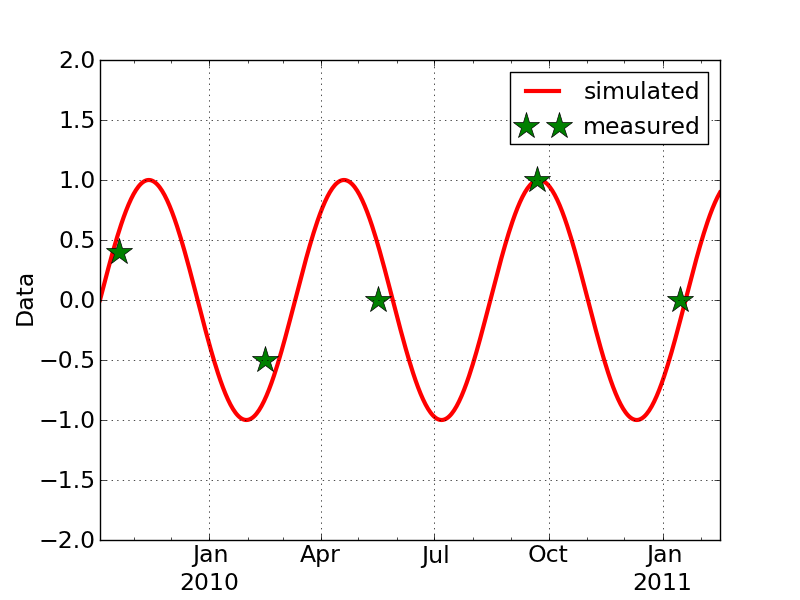
\includegraphics[width=0.5\textwidth]{images/date.png}
  \caption{Plot showing dates for x-axis.}
   \label{fig:date}
\end{figure}
\afterfig

\section{Bar charts}
\index{bar}
Let us first create some data. We will crate two variables (rainfall and runoff) of length 5. 
\beforeverb \begin{verbatim}
>>> import numpy as np
>>> import matplotlib.pyplot as plt
>>> n = 5
>>> rainfall_mean = 500+300*np.random.rand(n)
>>> runoff_mean = 0.75*np.random.rand(n)*rainfall_mean
\end{verbatim} \afterverb

The \verb"bar" requires the corresponding value for $x$, and it does not calculate by itself. We are also specifying the width of bars. The 
\verb"plt.bar" returns rectangle patches which can be used to modify  patches or to extract some information from them. In this example these rectangle patches are used to extract their height, and then to place text at the top of bars. Fig. \ref{fig:bar} shows the bar plot. 
\beforeverb \begin{verbatim}
>>> ind = np.arange(n)  # the x locations for the groups
>>> width = 0.35       # the width of the bars
>>> 
>>> rects1 = plt.bar(ind, rainfall_mean, width, color='g', label='Rainfall')
>>> rects2 = plt.bar(ind+width, runoff_mean, width, color='m', label='Runoff')
>>> 
>>> plt.ylabel('Annual sum (mm)')
>>> plt.title('Water balance')
>>> plt.xticks(ind+width, ('2001', '2002', '2003', '2004', '2005') )
>>> 
>>> def autolabel(rects):
>>>     # attach some text labels
>>>     for rect in rects:
>>>         height = rect.get_height()
>>>         plt.text(rect.get_x()+rect.get_width()/2., 1.05*height, '%d'%int(height),
>>>                 ha='center', va='bottom')
>>> 
>>> plt.legend()
>>> autolabel(rects1)
>>> autolabel(rects2)
>>> 
>>> plt.ylim(ymax=1000)
>>> plt.savefig('/home/tomer/my_books/python_in_hydrology/images/bar.png')
>>> plt.close()
\end{verbatim} \afterverb

\beforefig
\begin{figure}[h!]
  \centering
    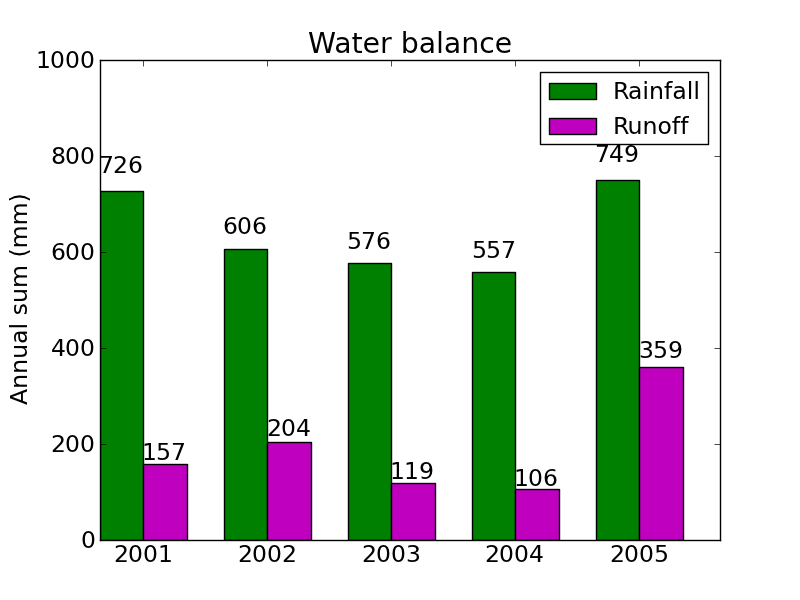
\includegraphics[width=0.5\textwidth]{images/bar.png}
  \caption{Plot showing an example of bar.}
   \label{fig:bar}
\end{figure}
\afterfig

\section{Pie charts}
\index{Pie}
First we generate three variables, runoff, recharge and evapotranspiration by assuming some rainfall. 
\beforeverb \begin{verbatim}
>>> rainfall = 1000
>>> runoff = 0.5*np.random.uniform()*rainfall
>>> recharge = 0.2*np.random.uniform()*rainfall
>>> evapotranspiration = rainfall - runoff - recharge
\end{verbatim} \afterverb
We modify the figure size by its default size to make the plot square. Then, we define the are for pie chart by specifying the \verb"plt.axis". 
\beforeverb \begin{verbatim}
>>> plt.figure(figsize=(8,8))
>>> plt.axis([0.2, 0.2, 0.8, 0.8])
\end{verbatim} \afterverb

We make a list of the variables, and tuple for the name of variables. 
\beforeverb \begin{verbatim}
>>> labels = 'Runoff', 'Recharge', 'Evapotranspiration'
>>> fracs = [runoff, recharge, evapotranspiration]
\end{verbatim} \afterverb

We can use explode to highlight some of the variable, in this case 'Recharge'. The amount of the explode is controlled by its parameters. The \verb"autopct" is used to define the format of the number inside pie. Fig. \ref{fig:pie} shows the pie chart. 
\beforeverb \begin{verbatim}
>>> explode=(0, 0.1, 0)
>>> plt.pie(fracs, explode=explode, labels=labels, autopct='%1.1f%%', shadow=True)
>>> plt.title('Annual water balance', bbox={'facecolor':'0.6', 'pad':10})
>>> plt.savefig('/home/tomer/my_books/python_in_hydrology/images/pie.png')
\end{verbatim} \afterverb

\beforefig
\begin{figure}[h!]
  \centering
    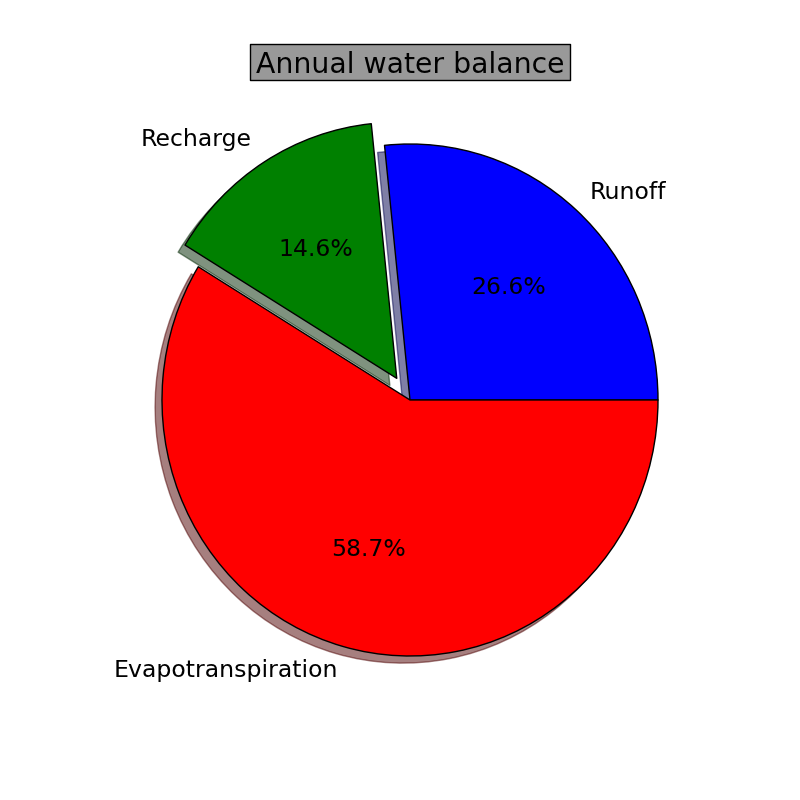
\includegraphics[scale=0.5]{images/pie.png}
  \caption{Plot showing an example of pie with explode.}
   \label{fig:pie}
\end{figure}
\afterfig

\section{2 D plots}
The images (JPEG, TIFF, PNG etc.) comes in two formats: greyscale or RGB. \verb"plt.imshow" can be used to show both type of images. First we use \verb"imread" to read the data from figures, then we make a three dimensional array data by first creating an empty array, and then specifying the each band data in RGB (red, green blue) order. If we are reading an image having all the three bands in a single image, the \verb"imread" will provide the data as three dimensional array and can be used directly. The \verb"imshow" is used to make the 2 dimensional plot with interpolation algorithm type to change its default interpolation type. Fig. \ref{fig:contourf} shows two dimensional map generated using the \verb"imshow". 
\beforeverb
\begin{verbatim}
>>> band2 = plt.imread('/home/tomer/my_books/python_in_hydrology/datas/band2.tif')
>>> band3 = plt.imread('/home/tomer/my_books/python_in_hydrology/datas/band3.tif')
>>> band4 = plt.imread('/home/tomer/my_books/python_in_hydrology/datas/band4.tif')
>>> 
>>> foo = np.empty((band2.shape[0], band2.shape[1], 3))
>>> foo[:,:,2] = band2
>>> foo[:,:,1] = band3
>>> foo[:,:,0] = band4
>>> 
>>> plt.imshow(foo, interpolation='hanning')
>>> plt.savefig('/home/tomer/my_books/python_in_hydrology/images/imshow.png')
\end{verbatim}
\afterverb
\index{imshow}

\beforefig
\begin{figure}[h!]
  \centering
    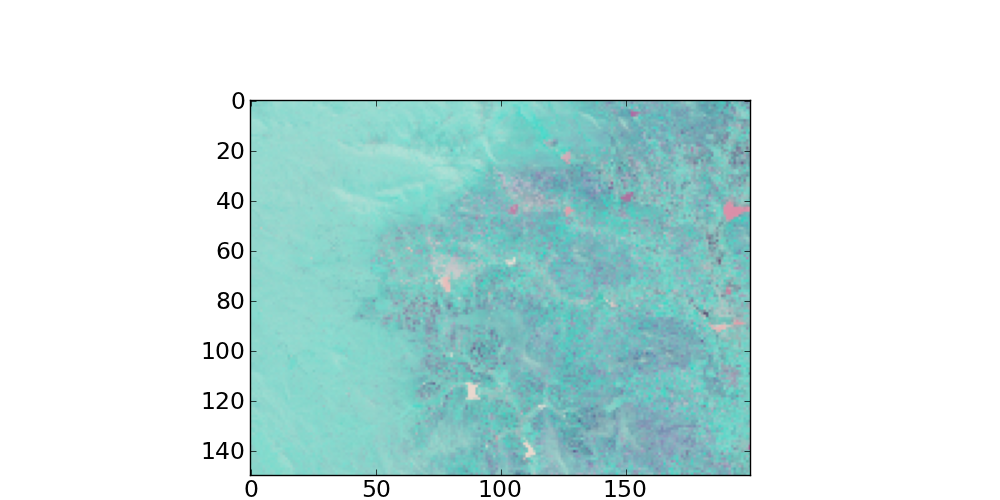
\includegraphics[scale=0.5]{images/imshow.png}
  \caption{Two dimensional plot using the imshow.}
   \label{fig:imshow}
\end{figure}
\afterfig

\verb"pcolor" stands for pseudo color, and is used to increase the contrast in the data while making plots. The \verb"colorbar" is used to show the colormap. The type of colormap is controlled by using the \verb"cmap" as input to \verb"pcolor". Fig. \ref{fig:pcolor} shows the pseudo color plot. 
\beforeverb \begin{verbatim}
>>> plt.pcolor(band2, cmap=plt.cm.Paired)
>>> plt.colorbar()
>>> plt.ylim(ymax=band2.shape[0])
>>> plt.savefig('/home/tomer/my_books/python_in_hydrology/images/pcolor.png')
\end{verbatim} \afterverb
\index{pcolor}

\beforefig
\begin{figure}[h!]
  \centering
    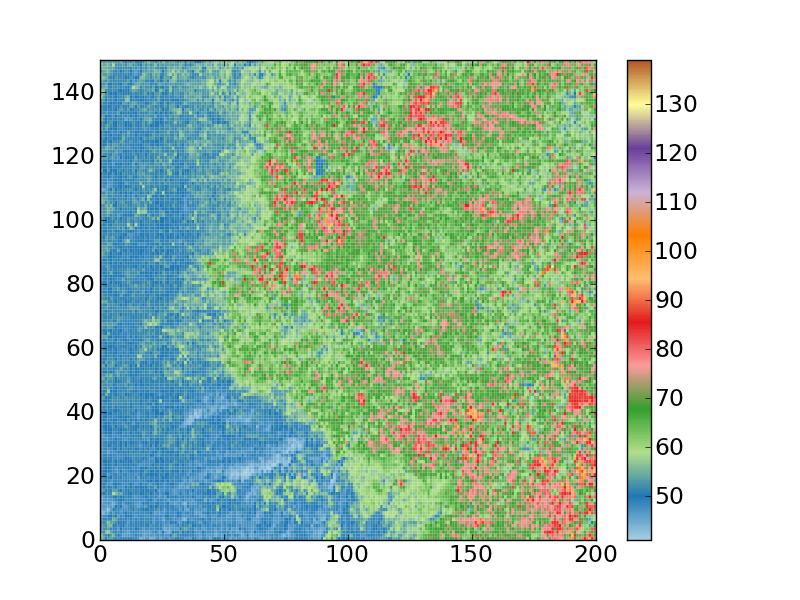
\includegraphics[scale=0.5]{images/pcolor.png}
  \caption{Two dimensional plot using the pcolor.}
   \label{fig:pcolor}
\end{figure}
\afterfig

We will be using the band2 data to make the contours. Since the 'band2' data has very hight spatial variability, we will be first filtering it using median filter. 
\beforeverb \begin{verbatim}
>>> from scipy.signal import medfilt2d
>>> data = medfilt2d(band2, kernel_size=7)
\end{verbatim} \afterverb
\index{Filter, Median}

\verb"plt.contour" is used to make contours. By default it does not show the contour values, to show the contour labels, we use the \verb"plt.clabel". Fig. \ref{fig:contour} shows the contour plot along with contour labels. 
\beforeverb \begin{verbatim}
>>> CS = plt.contour(data,10)
>>> plt.clabel(CS, inline=1, fontsize=10)
>>> plt.savefig('/home/tomer/my_books/python_in_hydrology/images/contour.png')
\end{verbatim} \afterverb
\index{contour}

\beforefig
\begin{figure}[h!]
  \centering
    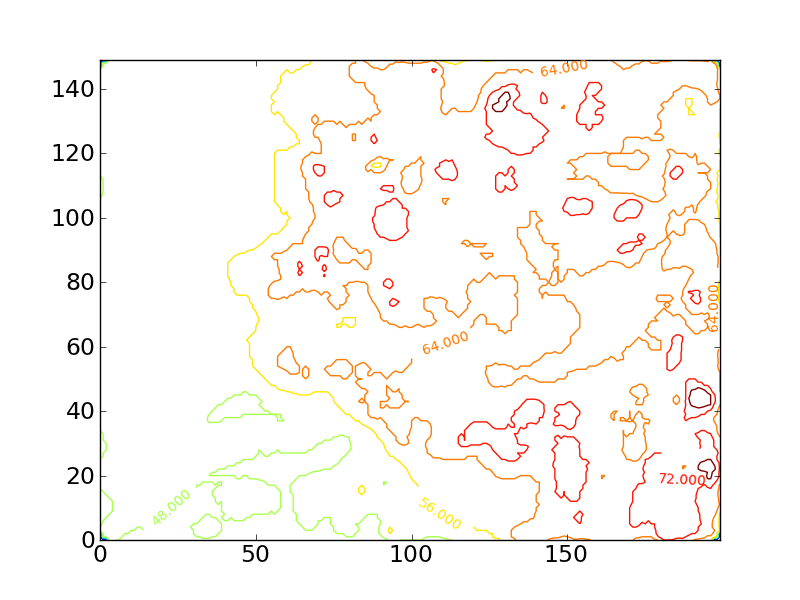
\includegraphics[scale=0.5]{images/contour.png}
  \caption{Plot showing the contour along with contour labels.}
   \label{fig:contour}
\end{figure}
\afterfig

\verb"plt.contour" provides the empty contour, i.e. there is no color between successive contours. We can use \verb"contourf" to make filled contour plots. Fig. \ref{fig:contourf} shows the filled contour plot. 
\beforeverb
\begin{verbatim}
>>> plt.contourf(data,10)
>>> plt.colorbar()
>>> plt.savefig('/home/tomer/my_books/python_in_hydrology/images/contourf.png')
\end{verbatim}
\afterverb
\index{contourf}

\beforefig
\begin{figure}[h!]
  \centering
    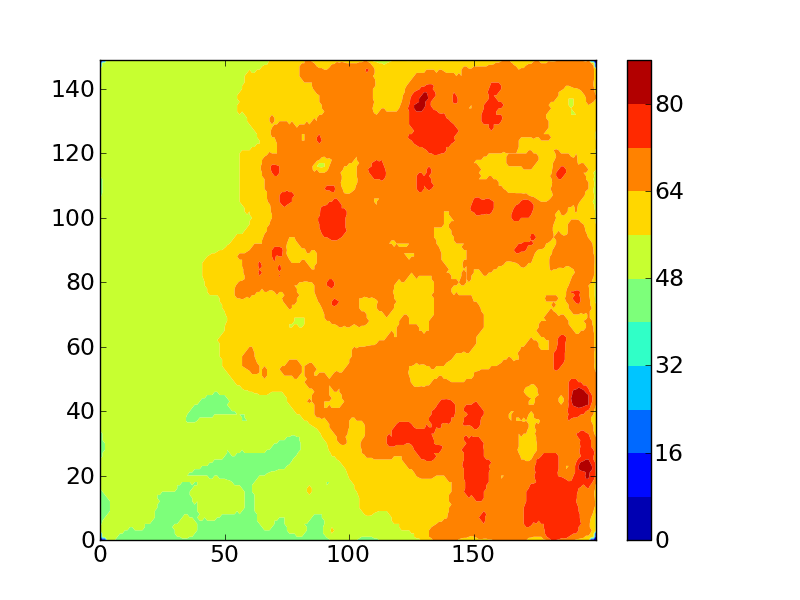
\includegraphics[scale=0.5]{images/contourf.png}
  \caption{Filled contour plotted using the contourf.}
   \label{fig:contourf}
\end{figure}
\afterfig

\section{3 D plots}
To make three dimensional plot, we need to import \verb"Axes3D" library from the \verb"mpl_toolkits.mplot3d". The scatter or line plot in three dimension is made in the way similar to two dimension. We will generate three variables, and make the three dimensional scatter plot. Fig. \ref{fig:3dscatter} shows the three dimensional scatter plot. 
\beforeverb \begin{verbatim}
>>> import numpy as np
>>> from mpl_toolkits.mplot3d import Axes3D
>>> 
>>> x = np.random.randn(100)
>>> y = np.random.randn(100)
>>> z = np.random.randn(100)
>>> 
>>> fig = plt.figure()
>>> ax = fig.add_subplot(111, projection='3d')
>>> ax.scatter(x, y, z, color='k', marker='s')
>>> 
>>> ax.set_xlabel('x')
>>> ax.set_ylabel('y')
>>> ax.set_zlabel('z')
>>> plt.savefig('/home/tomer/my_books/python_in_hydrology/images/3dscatter.png')
>>> plt.close()
\end{verbatim} \afterverb
\index{Plot, 3D}

\beforefig
\begin{figure}[h!]
  \centering
    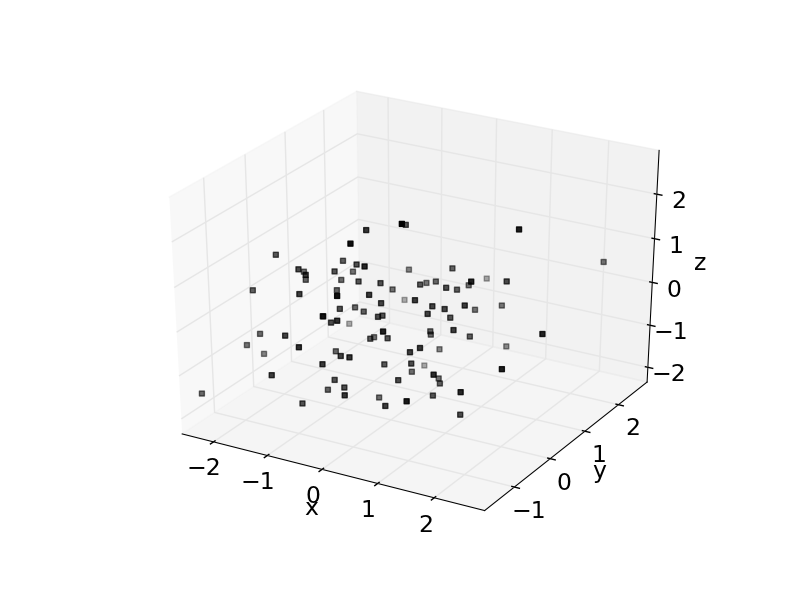
\includegraphics[scale=0.5]{images/3dscatter.png}
  \caption{Date axis}
   \label{fig:3dscatter}
\end{figure}
\afterfig

\section{Box-plot}
\index{Box-plot}
Box-plot is a way to graphically visualize the statistical properties of the data. It provides information about the minimum, first quartile (Q1), median (Q2), upper quartile (Q3), maximum, and outliers if present. \verb"boxplot" is used to make boxplot. Fig. \ref{fig:boxplot"} shows the box plot. 
\beforeverb \begin{verbatim}
>>> n = 4
>>> x = range(n)
>>> y = 5+np.random.randn(100,4)
>>> 
>>> plt.boxplot(y,'gD')
>>> plt.savefig('/home/tomer/my_books/python_in_hydrology/images/boxplot.png')
\end{verbatim} \afterverb

\beforefig
\begin{figure}[h!]
  \centering
    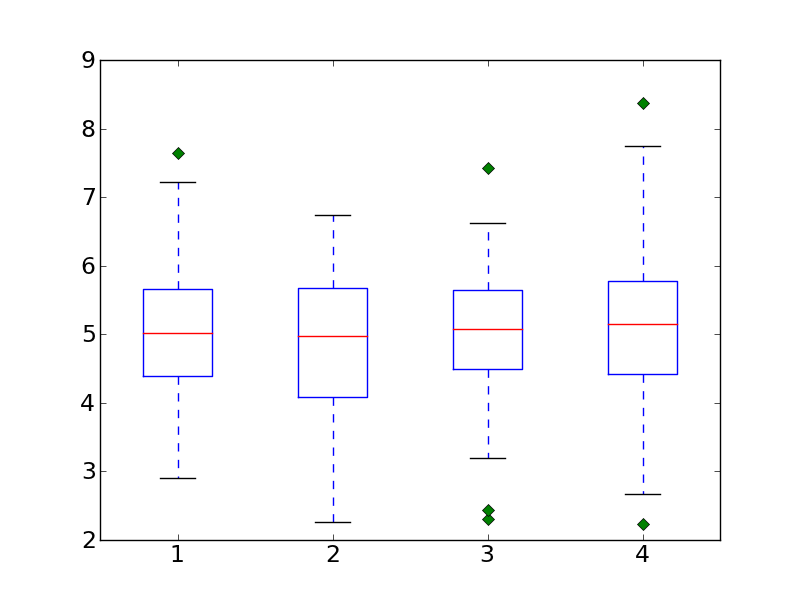
\includegraphics[scale=0.5]{images/boxplot.png}
  \caption{Box plot of data.}
   \label{fig:boxplot}
\end{figure}
\afterfig

\section{Q-Q plot}
\index{Q-Q plot}
The Q-Q (quantile-quantile) plot is a graphical method of comparing two probability distributions by plotting their quantiles against each other. We will use \verb"statistics" library to calculate the quantiles. We will generate three random variable, two having same (normal) distributions, and one having different (uniform) distribution, and will compare their behaviour on the Q-Q plot. Fig. \ref{fig:q_q} shows the Q-Q plot. On the x-axis we have the quantiles for normal distribution, on y-axis we are plotting quantiles of uniform and normal distributions. We  see that when the distributions are same, they fall on 1:1 line, otherwise they depart from it. 
\beforeverb \begin{verbatim}
>>> import statistics as st
>>> from scipy.interpolate import interp1d
>>> 
>>> def Q(data):
>>>     F, data1 = st.cpdf(data, n=1000)
>>>     f = interp1d(F, data1)
>>>     return f(np.linspace(0,1))
>>> 
>>> x = np.random.randn(1000)
>>> y = 5*np.random.rand(1000)
>>> z = np.random.randn(1000)
>>> 
>>> Qx = Q(x)
>>> Qy = Q(y)
>>> Qz = Q(z)
>>> 
>>> plt.plot([-5,5] , [-5,5], 'r', lw=1.5, label='1:1 line')
>>> plt.plot(Qx, Qy, 'gd', label='Uniform')
>>> plt.plot(Qx, Qz,  'm*', label='Normal')
>>> plt.axis((-5, 5, -5, 5))
>>> plt.legend(loc=2)
>>> plt.xlabel('Normal')
>>> plt.ylabel('observed')
>>> plt.savefig('/home/tomer/my_books/python_in_hydrology/images/q_q.png')
\end{verbatim} \afterverb

\beforefig
\begin{figure}[h!]
  \centering
    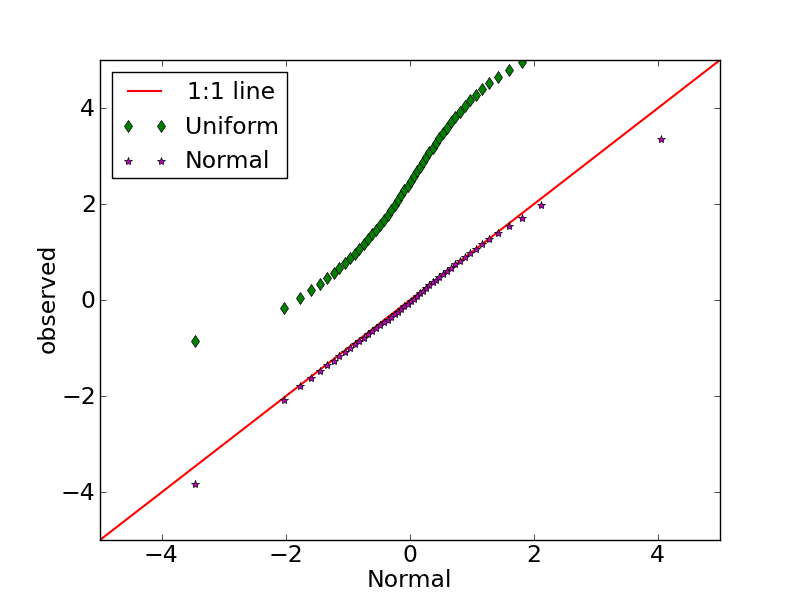
\includegraphics[scale=0.5]{images/q_q.png}
  \caption{Quantile-quantile plot.}
   \label{fig:q_q}
\end{figure}
\afterfig

\section{plotyy}
If we want to plot two variables in the same plot which have different range (minimum and maximum), then we should not plot them using same axis. If we do so, we will not be able to see the variation in one variable. Fig. \ref{fig:multi_y} shows the plot having two y axis. 
\beforeverb
\begin{verbatim}
>>> fig = plt.figure()
>>> plt.subplots_adjust(top=0.9,bottom=0.15,left=0.15,right=0.85)
>>> ax1 = fig.add_subplot(111)
>>> 
>>> t = np.linspace(0,10)
>>> y1 = 5*np.sin(t)
>>> y2 = 10*np.cos(t)
>>> 
>>> ax1.plot(t, y1, 'g', label='sin')
>>> ax1.set_xlabel('time (s)')
>>> 
>>> #Make the y-axis label and tick labels match the line color.
>>> ax1.set_ylabel('sin', color='b')
>>> for tl in ax1.get_yticklabels():
>>>     tl.set_color('b')
>>> ax1.set_ylim(-6,6)
>>> plt.legend(loc=3)
>>> 
>>> ax2 = ax1.twinx()
>>> ax2.plot(t, y2, 'r', label='cos')
>>> ax2.set_ylabel('cos', color='r')
>>> for tl in ax2.get_yticklabels():
>>>     tl.set_color('r')
>>> ax2.set_ylim(-15,15)    
>>> 
>>> plt.legend(loc=4)
>>> plt.savefig('/home/tomer/my_books/python_in_hydrology/images/multiple_y.png')
\end{verbatim}
\afterverb

\beforefig
\begin{figure}[h!]
  \centering
    \includegraphics[scale=0.5]{images/multiple_y.png}
  \caption{Plot showing multiple y-axis.}
   \label{fig:multi_y}
\end{figure}
\afterfig

\section{Annotation}
\index{Annotation}
Apart from plotting lines, dot, legends etc., we may need to put additional information on the plot. This is called annotation. We can put different arrow, texts etc. to make our graph more clear. Fig. \ref{fig:annotate} shows one such figure having few arrows, texts to improve the readability of the graph. 
\beforeverb \begin{verbatim}
>>> t = np.linspace(0,10)
>>> y = 5*np.sin(t)
>>> 
>>> plt.plot(t, y, lw=3, color='m')
>>> plt.xlabel('x')
>>> plt.ylabel('y')
>>> plt.annotate('ridge', xy=(np.pi/2, 5),  xycoords='data',
>>>             xytext=(-20, -75), textcoords='offset points',
>>>             arrowprops=dict(arrowstyle="->")
>>>             )
>>> 
>>> plt.annotate('valley', xy=(1.5*np.pi, -5),  xycoords='data',
>>>             xytext=(-30, 80), textcoords='offset points',
>>>             size=20,
>>>             bbox=dict(boxstyle="round,pad=.5", fc="0.8"),
>>>             arrowprops=dict(arrowstyle="->",),
>>>             )
>>> 
>>> plt.annotate('Annotation', xy=(8, -5),  xycoords='data',
>>>                 xytext=(-20, 0), textcoords='offset points',
>>>                 bbox=dict(boxstyle="round", fc="green"), fontsize=15)
>>> 
>>> plt.text(3.0, 0, "Down", color = "w", ha="center", va="center", rotation=90,
>>>             size=15, bbox=dict(boxstyle="larrow,pad=0.3", fc="r", ec="r", lw=2))
>>> 
>>> plt.text(np.pi*2, 0, "UP", color = "w", ha="center", va="center", rotation=90,
>>>             size=15, bbox=dict(boxstyle="rarrow,pad=0.3", fc="g", ec="g", lw=2))
>>> 
>>> plt.savefig('/home/tomer/my_books/python_in_hydrology/images/annotate.png')
\end{verbatim} \afterverb

\beforefig
\begin{figure}[h!]
  \centering
    \includegraphics[scale=0.5]{images/annotate.png}
  \caption{Plot showing various annotations.}
   \label{fig:annotate}
\end{figure}
\afterfig

\section{Basemap}
\index{Basemap}
The \verb"Basemap" library of \verb"mpl_toolkits.basemap" provides options for showing some variable on the globe, showing boundaries (hydrological, political etc.) in most commonly used projections. We will use plot the band1 data with the boundary of the Berambadi watershed. Fig. \ref{fig:basemap} shows the band1 data with boundary of watershed marked in white. 
\beforeverb \begin{verbatim}
>>> from mpl_toolkits.basemap import Basemap
>>> import gdal
>>> from gdalconst import *
>>> 
>>> # read the data
>>> dataset = gdal.Open("/home/tomer/my_books/python_in_hydrology/datas/band1.tif",GA_ReadOnly)
>>> band1 = dataset.GetRasterBand(1).ReadAsArray()
>>> GT = dataset.GetGeoTransform()
>>> 
>>> dataset = None
>>> 
>>> # make the co ordinate for the berambadi
>>> lon = np.linspace(GT[0]+GT[1]/2, GT[0]+GT[1]*(band1.shape[1]-0.5), band1.shape[1])
>>> lat = np.linspace(GT[3]+GT[5]/2, GT[3]+GT[5]*(band1.shape[0]-0.5), band1.shape[0])
>>> Lon, Lat = np.meshgrid(lon, lat)
>>> 
>>> # make the base map
>>> m = Basemap(projection='merc',llcrnrlat=11.72,urcrnrlat=11.825,\
>>>             llcrnrlon=76.51,urcrnrlon=76.67,lat_ts=20,resolution=None)
>>> 
>>> # draw parallels and meridians.
>>> m.drawparallels(np.arange(11.7,11.9,.05),labels=[1,0,0,0])
>>> m.drawmeridians(np.arange(76.4,76.8,.05),labels=[0,0,0,1])
>>> 
>>> # read the shapefile archive
>>> s = m.readshapefile('/home/tomer/my_books/python_in_hydrology/datas/berambadi','berambadi',
>>>     color='w',linewidth=2.5)
>>> 
>>> # compute native map projection coordinates of lat/lon grid.
>>> x, y = m(Lon,Lat)
>>> 
>>> # contour data over the map
>>> cs = m.pcolor(x,y,band1,cmap=plt.cm.jet)
>>> cb = plt.colorbar(cs, shrink=0.6, extend='both')
>>> 
>>> plt.title(" Band 1")
>>> plt.savefig('/home/tomer/my_books/python_in_hydrology/images/basemap.png')
\end{verbatim} \afterverb

\beforefig
\begin{figure}[h!]
  \centering
    \includegraphics[scale=0.5]{images/basemap.png}
  \caption{Spatial variation of band1 along with boundary of Berambadi watershed.}
   \label{fig:basemap}
\end{figure}
\afterfig


\section{Shared axis}
Often it is required to make two or more plots having the same axis ($x$ or $y$ or both). The \verb"plt.subplots" provides an easy way to make the common (shared) axis. First, we will generate the synthetic data having different range. Then plot using the \verb"plt.subplots". The other options in \verb"plt.subplots" are similar to \verb"plt.subplot". 
\beforeverb \begin{verbatim}
>>> x1 = range(100)
>>> x2 = range(125)
>>> 
>>> y1 = np.random.rand(100)
>>> y2 = 2.0*np.random.rand(125)
>>> y3 = np.random.rand(125)
>>> y4 = 1.5*np.random.rand(100)
>>> 
>>> fig, ((ax1, ax2), (ax3, ax4)) = plt.subplots(2, 2, sharex=True, sharey=True)
>>> ax1.plot(x1,y1, 'ro')
>>> ax2.plot(x2,y2, 'go')
>>> ax3.plot(x2,y3, 'bs')
>>> ax4.plot(x1,y4, 'mp')
>>> plt.tight_layout()
>>> plt.savefig('/home/tomer/my_books/python_in_hydrology/images/shared_xy.png')
\end{verbatim} \afterverb
Fig. \ref{fig:shared_xy} shows the resulted plot.

\beforefig
\begin{figure}[h!]
  \centering
    \includegraphics[scale=0.5]{images/shared_xy.png}
  \caption{Plots having the common (shared) axis.}
   \label{fig:shared_xy}
\end{figure}
\afterfig

\section{Subplot}
So far, we have used subplot having same width and height. The situation might arise, when we need to increase the size for some subplot. In the following section, we will try to plot such in such case. Firs, we will use \verb"plt.subplot", itself to make some particular subplot. 

\beforeverb \begin{verbatim}
>>> x = np.random.rand(25)
>>> y = np.arccos(x)
>>> 
>>> plt.close('all')
>>> plt.subplot(221)
>>> plt.scatter(x,y)
>>> 
>>> plt.subplot(223)
>>> plt.scatter(x,y)
>>> 
>>> plt.subplot(122)
>>> plt.scatter(x,y)
>>> plt.tight_layout()
>>> plt.savefig('/home/tomer/my_books/python_in_hydrology/images/sub_plot1.png')
\end{verbatim} \afterverb
Fig. \ref{fig:subplot1} shows the resulted plot. The \verb"plt.tight_layout()" increase the readability of the ticks labels. If this option is not used, then you might have got figures with overlapping labels etc. This options prevents overlapping of axis, title etc.

\beforefig
\begin{figure}[h!]
  \centering
    \includegraphics[scale=0.5]{images/sub_plot1.png}
  \caption{Plot with varying span of subplots.}
   \label{fig:subplot1}
\end{figure}
\afterfig

Now, we will make these kinds of subplot using \verb"subplot2grid". 
\beforeverb \begin{verbatim}
>>> fig = plt.figure()
>>> fig.subplots_adjust(wspace=0.5, hspace=0.4)
>>> 
>>> ax1 = plt.subplot2grid((3, 3), (0, 0))
>>> ax2 = plt.subplot2grid((3, 3), (0, 1), colspan=2)
>>> ax3 = plt.subplot2grid((3, 3), (1, 0), colspan=2, rowspan=2)
>>> ax4 = plt.subplot2grid((3, 3), (1, 2), rowspan=2)
>>> 
>>> ax1.scatter(10*x,y)
>>> ax2.scatter(10*x,y)
>>> ax3.scatter(10*x,y)
>>> ax4.scatter(10*x,y)
>>> plt.savefig('/home/tomer/my_books/python_in_hydrology/images/sub_plot2.png')
\end{verbatim} \afterverb
Fig. \ref{fig:subplot2} shows the resulted plot.

\beforefig
\begin{figure}[h!]
  \centering
    \includegraphics[scale=0.5]{images/sub_plot2.png}
  \caption{Plot with varying span of subplots plotted using subplot2grid.}
   \label{fig:subplot2}
\end{figure}
\afterfig

\chapter{Input-Output}
\section{xls}
\index{xls}
The \verb"data.xls" file contains the data of soil moisture estimated from the AMSR-E platform. You can open the xls file and have a look at its content. In this file we have data in two sheets, Ascending and Descending which corresponds to satellite direction. Each sheet contains the time series data for various grids point. Missing data is assigned a number of 999.9. In this section we will read data of one station for all the time, modify the data which is missing, and write in another xls file. We will be using \verb"xlsrd" library to read data from xls file, and \verb"xlwt" to write the data to xls file. The \verb"xlrd" does not read \verb"xlsx" data file, you should convert the \verb"xlsx" type of file into \verb"xls" before reading.

\beforeverb \begin{verbatim}
>>> import xlrd
>>> import numpy as np
\end{verbatim} \afterverb

We create book object by passing the name of xls file to \verb"xlrd.open_workbook". The sheet from which we need to read the data is specified using the \verb"sheet_by_name".  
\beforeverb \begin{verbatim}
>>> book = xlrd.open_workbook('/home/tomer/my_books/python_in_hydrology/datas/data.xls')
>>> sheet = book.sheet_by_name('Ascending')
\end{verbatim} \afterverb

The number of columns and rows in sheets can be checked by using the \verb"nrows" and \verb"ncols" attributes respectively. 
\beforeverb \begin{verbatim}
>>> sheet.nrows
1100
>>> sheet.ncols
39
\end{verbatim} \afterverb
Our sheet's first two rows are heading of table and latitude and longitude, and hence the length of time series data is two lesser than the number of rows. First we create an empty array to store the data, and then we read the data cell by cell using the \verb"cell_value". We will be reading the data of grid having latitude equal to 12.4958 and longitude equal to 75.7484, which is in fourth column (indices start with zero). 
\beforeverb \begin{verbatim}
>>> sm = np.empty(sheet.nrows-2)
>>> year = np.empty(sheet.nrows-2, int)
>>> month = np.empty(sheet.nrows-2, int)
>>> day = np.empty(sheet.nrows-2, int)
>>> for i in range(sm.shape[0]): 
>>>    sm[i] = sheet.cell_value(i+2,27)  
>>>    year[i] = sheet.cell_value(i+2,0)
>>>    month[i] = sheet.cell_value(i+2,1)
>>>    day[i] = sheet.cell_value(i+2,2)
\end{verbatim} \afterverb
We can check the data of some variable e.g. sm.
\beforeverb \begin{verbatim}
>>> sm
array([  16.6,  999.9,   15.3, ...,   17.4,  999.9,   18.2])
\end{verbatim} \afterverb
We can define all the missing data as nan. 
\beforeverb \begin{verbatim}
>>> sm[sm==999.9] = np.nan
>>> sm
array([ 16.6,   nan,  15.3, ...,  17.4,   nan,  18.2])
\end{verbatim} \afterverb
Now the soil moisture data has nan instead of 999.9 to denote missing values. We will write this soil moisture data into xls file using \verb"xlwt" library. First we open a workbook, then we add a sheet by name using \verb"add_sheet". After this we start writing entries cell by cell. Finally, we save the worksheet using \verb"book.save". 

\beforeverb \begin{verbatim}
>>> import xlwt
>>> book = xlwt.Workbook()
>>> sheet = book.add_sheet('Ascending')
>>> sheet.write(0,0, 'Year')
>>> sheet.write(0,1, 'Month')
>>> sheet.write(0,2, 'Day')
>>> sheet.write(0,3, 'Latitude')
>>> sheet.write(1,3, 'Longitude')
>>> 
>>> for i in range(len(sm)):
>>>     sheet.write(i+2, 4, sm[i])
>>>     sheet.write(i+2, 0, year[i])
>>>     sheet.write(i+2, 1, month[i])
>>>     sheet.write(i+2, 2, day[i])
>>>     
>>> book.save('/home/tomer/my_books/python_in_hydrology/datas/data1.xls')
\end{verbatim} \afterverb

I have written a library \verb"ambhas.xls" which provides relatively easy way to read and write the xls data. The data can be read in the following way. 
\beforeverb \begin{verbatim}
>>> from ambhas.xls import xlsread
>>> fname = '/home/tomer/my_books/python_in_hydrology/datas/data.xls'
>>> foo = xlsread(fname)
>>> data = foo.get_cells('a3:a5', 'Ascending')
\end{verbatim} \afterverb

The data to \verb"xls" file is written in the following way. The data which is written should be a numpy array.
\beforeverb \begin{verbatim}
>>> from ambhas.xls import xlswrite
>>> fname = '/home/tomer/my_books/python_in_hydrology/datas/data.xls'
>>> foo = xlswrite(data, 'a3', 'Ascending')
>>> foo.save(fname)
\end{verbatim} \afterverb
As this library depends upon the \verb"xlrd", it also does not read \verb"xlsx" data file, and you should convert the \verb"xlsx" type of file into \verb"xls" before reading.

\section{Text file}
\index{Text file}
Some of the software/tools take the input form text files and then write to text files. If we want to do bath processing (process many files) using these tools, then we need to modify the input text files and extract the information from the file written by the tool. In this section we will read a file, and then change some parameter of the file, and then write it.\\

Before jumping into many thing, first we will just read the text file. The 'r' is for reading, 'w' is for 'writing' and 'a' is for appending into existing file. 
\beforeverb \begin{verbatim}
>>> fname_read = '/home/tomer/my_books/python_in_hydrology/datas/Albedo.prm'
>>> f_read = open(fname_read, 'r')
>>> for line in f_read:
>>>     print line
>>> f_read.close()
NUM_RUNS = 1



BEGIN

INPUT_FILENAME = /home/tomer/data/input.hdf

OBJECT_NAME = MOD_Grid_BRDF|

FIELD_NAME = Albedo_BSA_Band1

BAND_NUMBER = 1

SPATIAL_SUBSET_UL_CORNER = ( 13.0 75.0 )

SPATIAL_SUBSET_LR_CORNER = ( 11.0 78.0 )

RESAMPLING_TYPE = BI

OUTPUT_PROJECTION_TYPE = UTM

ELLIPSOID_CODE = WGS84

UTM_ZONE = 0

OUTPUT_PROJECTION_PARAMETERS = ( 0.0 0.0 0.0 0.0 0.0 0.0 0.0 0.0 0.0 0.0 0.0 0.0 0.0 0.0 0.0  )

OUTPUT_FILENAME = /home/tomer/data/output.tif

OUTPUT_TYPE = GEO

END
\end{verbatim} \afterverb
We see that file has many parameters defined, which will be used by some tool to process input hdf images. Let us say, we have four input files, and we want to batch process them.

\beforeverb \begin{verbatim}
>>> fname_input = ['input0', 'input1', 'input2', 'input3']
>>> fname_output = ['output0', 'output1', 'ouput2', 'output3']
>>> 
>>> for i in range(len(fname_input)):
>>>     
>>>     fname_read = '/home/tomer/my_books/python_in_hydrology/datas/Albedo.prm'
>>>     f_read = open(fname_read, 'r')
>>> 
>>>     fname_write = '/home/tomer/my_books/python_in_hydrology/datas/Albedo_ii.prm'.replace('ii',str(i))
>>>     f_write = open(fname_write, 'w')
>>>     for line in f_read:
>>>         if 'INPUT_FILENAME' in line:
>>>             line = line.replace('input',fname_input[i])
>>>             print line
>>>         if 'OUTPUT_FILENAME' in line:
>>>             line = line.replace('output',fname_output[i])
>>>             print line
>>>         f_write.write(line)
>>>         
>>>     f_write.close()
>>> 
>>> f_read.close()
\end{verbatim} \afterverb

\section{NetCDF}
\index{NetCDF}
In this section, we will read a NetCDF file, and write in the same format. I am using the file, \emph{rhum.2003.nc} which can be downloaded from \url{http://www.unidata.ucar.edu/software/netcdf/examples/files.html}. We will be using \verb"NetCDF" library from \verb"Scientific.IO" to read and write the NetCDF data, so lets first import it.
\beforeverb \begin{verbatim}
>>> import numpy as np
>>> from Scientific.IO import NetCDF as nc
\end{verbatim} \afterverb

First, we open the file. 
\beforeverb \begin{verbatim}
>>> file = nc.NetCDFFile('/home/tomer/my_books/python_in_hydrology/datas/rhum.2003.nc', 'r')
\end{verbatim} \afterverb

We can look at its attributes by using \verb"dir".
\beforeverb \begin{verbatim}
>>> dir(file)
['Conventions', 'base_date', 'close', 'createDimension', 'createVariable', 'description', 
'flush', 'history', 'platform', 'sync', 'title']
\end{verbatim} \afterverb

The \verb"title" tells about the title of dataset, description provides the description of the content of file. 
\beforeverb \begin{verbatim}
>>> file.title
'mean daily NMC reanalysis (2003)'
>>> file.description
'Data is from NMC initialized reanalysis\n(4x/day).  It consists of most variables interpolated to\npressure surfaces from model (sigma) surfaces.'
\end{verbatim} \afterverb

We can look at the dimension of the data.
\beforeverb \begin{verbatim}
>>> file.dimensions
{'lat': 73, 'time': None, 'lon': 144, 'level': 8}
\end{verbatim} \afterverb
We see that, the data has four dimensions: lat, time, lon, and level. The size of each dimensions is also given. Now, we can look at the variables in the data.

\beforeverb \begin{verbatim}
>>> file.variables
{'lat': <NetCDFVariable object at 0x1d33270>, 'rhum': <NetCDFVariable object at 0x1d33030>, 'time': <NetCDFVariable object at 0x1d33348>, 'lon': <NetCDFVariable object at 0x1d336f0>, 'level': <NetCDFVariable object at 0x1d33858>}
\end{verbatim} \afterverb

This provides, the name of variables and a reference of the variable to the data. This means that this does not load the data into memory, in fact just provide a reference in the file, and we can retrieve only the variable that we want. We shall get the value of 'rhum' variable. First we the reference to some variable name. Then we can see its unit, data type, and get its value.
\beforeverb \begin{verbatim}
>>> foo = file.variables['level']
>>> foo.units
'%'
>>> foo.typecode
'h'
>>> rhum = foo.getValue
\end{verbatim} \afterverb

Now, we can look at the shape of the variable 'rhum'.
\beforeverb \begin{verbatim}
>>> rhum.shape
(365, 8, 73, 144)
\end{verbatim} \afterverb
The first dimension represent the time, second represent the various pressure levels, and third represent the latitude, and the last one is longitude. 

We can write the file in the same way. First we open the file for writing. 
\beforeverb \begin{verbatim}
>>> file = nc.NetCDFFile('/home/tomer/my_books/python_in_hydrology/datas/test.nc', 'w')
\end{verbatim} \afterverb

Then we can define some global attributes like title, description etc.
\beforeverb \begin{verbatim}
>>> setattr(file, 'title', 'trial')
>>> setattr(file, 'description', 'File generated while tesing to write in NetCDF')
\end{verbatim} \afterverb

Now, we can create some dimensions. We need to define the name of dimension and their size. 
\beforeverb \begin{verbatim}
>>> file.createDimension('lat', 73) 
>>> file.createDimension('lon', 144) 
>>> file.createDimension('level', 8) 
>>> file.createDimension('time', 365) 
\end{verbatim} \afterverb

Now, we can save the variables. First, we need to define the dimension from the list created above. The dimension should be tuple, notice the comma after the \verb" 'lat', ". After this, we can create variable using \verb"createVariable", we need to specify the name of variable, format and dimension. We see that it has created a variable named 'lat' and is referring to it.
\beforeverb \begin{verbatim}
>>> varDims = 'lat',
>>> lat = file.createVariable('lat', 'f', varDims)
>>> print(file.variables)
{'lat': <NetCDFVariable object at 0x2c39078>}
\end{verbatim} \afterverb

Finally, we can assign our data to this variable. 
\beforeverb \begin{verbatim}
>>> lat = np.random.rand(73)
\end{verbatim} \afterverb
Now, we can close the file.
\beforeverb \begin{verbatim}
>>> file.close()
\end{verbatim} \afterverb

\section{Pickle}
\index{Pickle}
\verb"Pickle" format is very fast to read and write. But it is only useful when you want to keep data for yourself, e.g. write data from one program, and read the same data into another program. First we import \verb"cPicle" and call it \verb"pickle". 
\beforeverb \begin{verbatim}
>>> import cPickle as pickle
\end{verbatim} \afterverb

We define one variable e.g. a list and first save it and then read it.
\beforeverb \begin{verbatim}
>>> var = [2, 5, 8, 'foo']
\end{verbatim} \afterverb

We use \verb"pickle.dump" to save the data. 
\beforeverb \begin{verbatim}
>>> var = [2, 5, 8, 'foo']
>>> pickle.dump(var, open( "/home/tomer/my_books/python_in_hydrology.pkl", "wb" ) )
>>> 
>>> var1 = pickle.load( open( "/home/tomer/my_books/python_in_hydrology.pkl", "rb" ) )
>>> print(var1)
[2, 5, 8, 'foo']
\end{verbatim} \afterverb

\chapter{Numerical Modelling}

\section{Integration}
\index{Integration}
Suppose we want to integrate some function and the function can not be integrated analytical, then we go for numerical integration. To check if our numerical integration schemes is working properly or not, we integrate the function for which analytical solution is available and then we compare our solution. So let us begin with function of one variable. Suppose, we have function $f(x) = x$ to integrate over limit 0 to 10. We know from mathematics that the answer is 50. Let us now try numerical methods about the solution. We will use \verb"integrate" library of \verb"scipy". For simple function we can use \verb"lambda" function instead of \verb"def" to define the function. The function \verb"integrate.quad" perform our task. It returns the integration and error in integration.
\beforeverb \begin{verbatim}
>>> from scipy import integrate
>>> y_fun = lambda x: x
>>> y,err = integrate.quad(x2,0,10)
>>> print(y,err)
(50.0, 5.551115123125783e-13)
\end{verbatim} \afterverb

We get the 50.0 as answer which is exactly the analytical solution, and also it says that error is the solution is very low. It could be by chance, that we get accurate solution from the numerical scheme. So let us try one more function, this time exponential. We will integrate $f(x)=exp(-x)$ over 0 to $\infty$. 
\beforeverb \begin{verbatim}
>>> y_func = lambda x: np.exp(-x)
>>> y = integrate.quad(y_func, 0, np.inf)
>>> print(y)
(1.0000000000000002, 5.842606742906004e-11)
\end{verbatim} \afterverb
We see that the solution is very near to the analytical solution (1.0). These function had only the variable as input, but we may want to have additional parameter in the function, e.g. $f(x)=exp(-ax$, and assume $a=0.5$ for this example. The \verb"integrate.quad" provides options for providing additional argument also. 
\beforeverb \begin{verbatim}
f = lambda x,a : np.exp(-a*x)
y, err = integrate.quad(f, 0, 1, args=(0.5,))
>>> y
0.786938680574733
\end{verbatim} \afterverb


\section{ODE}
\index{ODE}
Let us solve the ordinary differential equation, given as:
\begin{equation}
\frac{dy}{dt} = -xt,
\end{equation}
with,
\begin{equation}
y_0 = 10.
\end{equation}

First, we can import required libraries.
\beforeverb \begin{verbatim}
>>> import numpy as np
>>> from scipy import integrate
>>> import matplotlib.pyplot as plt
\end{verbatim} \afterverb

Now, we define our function, and the timer at which we want the solution. 
\beforeverb \begin{verbatim}
>>> y1 = lambda x,t : -x*t
>>> t = np.linspace(0,10)
\end{verbatim} \afterverb

Now, we can use \verb"integrate.odeint" to solve the ordinary differential equation. Then, we can make a plot of the solution with respect to the time. 
\beforeverb \begin{verbatim}
>>> y = integrate.odeint(y1, 10, t)
>>> # plot
>>> plt.plot(t,y)
>>> plt.xlabel('x')
>>> plt.ylabel('y')
>>> plt.savefig('/home/tomer/my_books/python_in_hydrology/images/ode.png')
\end{verbatim} \afterverb

Fig. \ref{fig:ode} shows the variation of $y$ over time. 

\beforefig
\begin{figure}[h!]
  \centering
    \includegraphics[scale=0.5]{images/ode.png}
  \caption{Variation of $y$ over time.}
   \label{fig:ode}
\end{figure}
\afterfig

Let us, solve a system of ordinary differential equation given as,
\begin{equation}
\frac{dx}{dt} = Ax,
\end{equation}
where,
\begin{equation}
A = \begin{bmatrix}
  -D_1 & D_1 & 0 \\
  D_1 & -D_1-D_2 & D_2 \\
  0 & D_2 & -D_3\\
 \end{bmatrix}
\end{equation}

We begin with defining the parameters and $A$ matrix. 
\beforeverb \begin{verbatim}
>>> D = [0.2, 0.1, 0.3]
>>> A = np.array([[D[0], -D[0], 0],
>>>              [D[0], -D[0]-D[1], D[1]],
>>>              [0, D[2], -D[2]]])
\end{verbatim} \afterverb

Now, we can define our function $dx/dt$. 
\beforeverb \begin{verbatim}                 
>>> def dX_dt(sm, t=0):
>>>     return np.dot(A,sm)
\end{verbatim} \afterverb

Finally, we define time, initial condition, use \verb"integrate.odeint" to solve, and then plot. 
\beforeverb \begin{verbatim}     
>>> t = np.linspace(0, 10, 100)    
>>> X0 = np.array([10, 5, 20]) 
>>> X, infodict = integrate.odeint(dX_dt, X0, t, full_output=True)
>>> 
>>> plt.plot(t,X)
>>> plt.xlabel('Time')
>>> plt.ylabel('X')
>>> plt.legend(['X1','X2','X3'])
>>> plt.savefig('/home/tomer/my_books/python_in_hydrology/images/ode_system.png')
\end{verbatim} \afterverb

\beforefig
\begin{figure}[h!]
  \centering
    \includegraphics[scale=0.5]{images/ode_system.png}
  \caption{Variation of $x$ over time.}
   \label{fig:ode}
\end{figure}
\afterfig

\section{Parameter Estimation}
\index{Parameter Estimation}
\beforeverb \begin{verbatim}
>>> from scipy import optimize, special
>>> x = np.arange(0,10,0.01)
>>> for k in np.arange(0.5,5.5):
>>>     y = special.jv(k,x)
>>> 
>>> f = lambda x: -special.jv(k,x)
>>> x_max = optimize.fminbound(f,0,6)
>>> 
>>> plt.plot(x,y, lw=3)
>>> plt.plot([x_max], [special.jv(k,x_max)],'rs', ms=12)
>>> plt.title('Different Bessel functions and their local maxima')
>>> plt.savefig('/home/tomer/my_books/python_in_hydrology/images/inverse.png')
>>> plt.close()
\end{verbatim} \afterverb
\index{fminbound}

\beforefig
\begin{figure}[h!]
  \centering
    \includegraphics[scale=0.5]{images/inverse.png}
  \caption{Demonstration of inverse modelling.}
   \label{fig:inverse}
\end{figure}
\afterfig

\chapter{Advance statistics}

\section{copula}
Copulas are used to describe the dependence between random variables. Copula means coupling two CDFs. Let us generate two random variables; one having normal distribution, another combination of first one and uniform distribution.

\beforeverb \begin{verbatim}
>>> import numpy as np
>>> import matplotlib.pyplot as plt
>>> from matplotlib.ticker import NullFormatter
>>> 
>>> # synthetic data
>>> x = np.random.randn(1000)
>>> y = np.random.randn(1000)
\end{verbatim} \afterverb

First we would like to how is our data related by using scatter plot, and also we would like to see how is the distribution of $x$ and $y$. We can do this in three separate plots, or using subplots. In the present case we will trying this in one plot by specifying different axis for these 3 plots. We begin with defining the axis limits for our three plots. The input to \verb"axis" are $x$ and $y$ for the lower left corner, width and height of the plot. in the following example we are specifying axis in such as way so that plots are aligned properly. 

\beforeverb \begin{verbatim}
>>> plt.clf()
>>> axScatter = plt.axes([0.1, 0.1, 0.5, 0.5])
>>> axHistx = plt.axes([0.1, 0.65, 0.5, 0.3])
>>> axHisty = plt.axes([0.65, 0.1, 0.3, 0.5])
\end{verbatim} \afterverb

Now, we use this axis to make plots. 
\beforeverb \begin{verbatim}
>>> # the plots
>>> axScatter.scatter(x, y)
>>> axHistx.hist(x)
>>> axHisty.hist(y, orientation='horizontal')
>>> 
>>> # set the limit of histogram plots
>>> axHistx.set_xlim( axScatter.get_xlim() )
>>> axHisty.set_ylim( axScatter.get_ylim() )
>>> 
>>> plt.savefig('/home/tomer/my_books/python_in_hydrology/images/copula_1.png')
\end{verbatim} \afterverb

Fig. \ref{fig:copula1} shows the resulted plot. 
\beforefig
\begin{figure}[h!]
  \centering
    \includegraphics[scale=0.5]{images/copula_1.png}
  \caption{Scatter plot along with marginal histograms.}
   \label{fig:copula1}
\end{figure}
\afterfig

Now, let us try to simulate ensemble of data using copula. I have written a library, \verb"ambhas.copula" to deal with copulas. This library has three copulas (Frank, Clayton, and Gumbel) in it. First we import the library, then we initialize the class. 

\beforeverb \begin{verbatim}
>>> from ambhas.copula import Copula
>>> foo = Copula(x, y, 'frank')
\end{verbatim} \afterverb

We can get the value of Kendall's tau, and the parameter of Frank copula by attributes \verb"tau" and \verb"theta" respectively. 
\beforeverb \begin{verbatim}
>>> print(foo.tau)
0.179797979798
>>> print(foo.theta)
1.66204833984
\end{verbatim} \afterverb

We can generate the ensemble using Frank copula. 
\beforeverb \begin{verbatim}
>>> x1,y1 = foo.generate_xy()
\end{verbatim} \afterverb

Now, we can plot the simulated data with original data.
\beforeverb \begin{verbatim}
>>> plt.scatter(x1,y1, color='g')
>>> plt.scatter(x,y, color='r')
>>> plt.xlabel('x')
>>> plt.ylabel('y')
>>> plt.savefig('/home/tomer/my_books/python_in_hydrology/images/copula_2.png')
\end{verbatim} \afterverb

Fig. \ref{fig:copula2} shows the resulted plot. 
\beforefig
\begin{figure}[h!]
  \centering
    \includegraphics[scale=0.5]{images/copula_2.png}
  \caption{Simulated ensemble along with original data.}
   \label{fig:copula2}
\end{figure}
\afterfig

\section{Multivariate distribution}
So far, we have generated random variables with only univariate distribution. In this section we will be generating multivariate nominally distributed random variable by specifying the mean and covariance matrix to \verb"np.random.multivariate_normal". 
\beforeverb \begin{verbatim}
>>> mean = [0,5]
>>> cov = [[1,0.4],[0.4,1]]
>>> data = np.random.multivariate_normal(mean,cov,5000)
\end{verbatim} \afterverb

We can check its mean and covariance.
\beforeverb \begin{verbatim}
>>> print(data.mean(axis=0))
[ 0.00814047  5.00406784]
>>> print(np.corrcoef(data.T))
[[ 1.          0.40707918]
 [ 0.40707918  1.        ]]
\end{verbatim} \afterverb
We see that generated random variable had mean and covariance close to the specified input. 


\section{Kriging}
Kriging is a widely used method for interpolation in hydrology apart from other areas. The advantage of Kriging over other interpolation method e.g. linear interpolation, radial basis function and  spline etc. is that Kriging methodology provides a way to estimate the parameter of interpolation and also provides the uncertainty in the interpolated values. The Kriging methodology involves two steps: (i) estimation of variogram and fitting a theortical variogram to it, and (ii) performing the interpolation. The empirical variogram reveals many interesesting thing about the data and sampling intervals. It is worthwhile to look into these aspects. So, first we begin by generating different type of synthetic dataset to understand the variogram. The example taken in this are from the book, 'Introduction to Geostatistics' by P. K. Kitanidis. The python library used for Kriging is \verb"ambhas.krige".\\

First, we consider the case when the scale of variability is larger than the scale of sampling. Consider the variable,
\begin{equation}
z(x) = cos(2 x/0.001).
\end{equation}
Where, $x$ is sampled 100 times from the uniform distribution in the range 0 to 1. Because the \verb"ambhas.krige" library work only on two dimensional data, we will generate one more variable $y$ apart from $x$ and $y$. The value of $y$ will be constant as to mimic only one dimensional effects. The python code to generate the synthetic data is:

\beforeverb \begin{verbatim}
>>> # import required library
>>> import numpy as np
>>> import matplotlib.pyplot as plt
>>> 
>>> x = np.random.rand(100) # uniformly distributed x
>>> y = np.ones(x.shape) 
>>> z = np.cos(2*np.pi*x/0.001) 
\end{verbatim} \afterverb

Let us have a look at the generated synthetic data. The resulted plot is shown in Fig. \ref{fig:krige_1}. 

\beforeverb \begin{verbatim}
>>> plt.clf()
>>> plt.plot(x,z, 'ro')
>>> plt.xlabel('x')
>>> plt.ylabel('z')
>>> plt.savefig('/home/tomer/svn/python-in-hydrology/images/krige_1.png')
\end{verbatim} \afterverb

\beforefig
\begin{figure}[h!]
  \centering
    \includegraphics[scale=0.5]{images/krige_1.png}
  \caption{The variation in $z$ with respect to $x$.}
   \label{fig:krige_1}
\end{figure}
\afterfig

We begin with importing the \verb"ambhas.krige" library. The we use its function Ordinary Kriging which is defined by name \verb"OK" to make an instance of Kriging class. To view the variogram, we use the \verb"variogram" method. There are two types of variogram available, first one is the raw variogram, i.e. the averaging over the data is not performed, second one is averaged over uniform intervals of lag distance. Let us first look how the raw variogram looks like. 

\beforeverb \begin{verbatim}
>>> from ambhas import krige
>>> foo = krige.OK(x,y,z)
>>> D,G = foo.variogram(var_type='scattered')
>>> 
>>> plt.clf()
>>> plt.plot(D,G, '.')
>>> plt.xlabel('lag distance')
>>> plt.ylabel('variogram')
>>> plt.savefig('/home/tomer/svn/python-in-hydrology/images/krige_2.png')
\end{verbatim} \afterverb

The raw variogarm is shown in Fig. \ref{fig:krige_2}. This variogram is very scattered and does not provide any insight into the behaviour of the data. To look into the behaviour of the data, we use averaged variogram. 

\beforefig
\begin{figure}[h!]
  \centering
    \includegraphics[scale=0.5]{images/krige_2.png}
  \caption{Raw variogram.}
   \label{fig:krige_2}
\end{figure}
\afterfig

The averaged variogram (or simply called variogram) is estimated by giving the \verb"averaged" as input to the argument \verb"var_type" of \verb"variogram" method. The variogram is shown in Fig. \ref{fig:krige_3}. The variogram looks nearly flat. It means that the behaviour is same at any lag distance, or the variable ($z$) has same variability at any scale. This could happen because of either the variable is like this, or that our sampling is so poor that we are unable to capture the behaviour of variable. 

\beforeverb \begin{verbatim}
>>> DE, GE = foo.variogram(var_type='averaged', min_lag=0.025)
>>> 
>>> plt.clf()
>>> plt.plot(DE,GE, 'ro')
>>> plt.xlabel('lag distance')
>>> plt.ylabel('variogram')
>>> plt.ylim((0,1))
>>> plt.savefig('/home/tomer/svn/python-in-hydrology/images/krige_3.png')
\end{verbatim} \afterverb

\beforefig
\begin{figure}[!h]
  \centering
    \includegraphics[scale=0.5]{images/krige_3.png}
  \caption{Variogram.}
   \label{fig:krige_3}
\end{figure}
\afterfig

Let us try another variable that has variability at larger scaler than our sampling. We keep the same sampling, and change the variability of the signal in the following way:
\begin{equation}
z(x) = cos(2 x/0.25).
\end{equation}

\beforeverb \begin{verbatim}
>>> x = np.random.rand(100) # uniformly distributed x
>>> y = np.ones(x.shape) 
>>> z = np.cos(2*x/0.25) 
>>> 
>>> plt.clf()
>>> plt.plot(x,z, 'ro')
>>> plt.xlabel('x')
>>> plt.ylabel('z')
>>> plt.savefig('/home/tomer/svn/python-in-hydrology/images/krige_4.png')
\end{verbatim} \afterverb

Fig. \ref{fig:krige_4} shows the signal. In the figure, we see that data shows a nice patterns. The visibility of patterns come from either the data really has some pattern or the sampling is good enough. As we have seen in last example the raw variogram is very cluttered, so we plot only the averaged variogram. 

\beforefig
\begin{figure}[h!]
  \centering
    \includegraphics[scale=0.5]{images/krige_4.png}
  \caption{The variation of $z$ with $x$.}
   \label{fig:krige_4}
\end{figure}
\afterfig


\beforeverb \begin{verbatim}
>>> foo = krige.OK(x,y,z)
>>> DE,GE = foo.variogram(var_type='averaged', min_lag=0.025)
>>> 
>>> plt.clf()
>>> plt.plot(DE,GE, 'r--o')
>>> plt.xlabel('lag distance')
>>> plt.ylabel('variogram')
>>> plt.ylim((0,1))
>>> plt.savefig('/home/tomer/svn/python-in-hydrology/images/krige_5.png')
\end{verbatim} \afterverb

The resulted variogram is shown in Fig. \ref{fig:krige_5}. The variogram shows a clear trend. The variability is increasing as the lag distance is increasing. This means that the variability is higher at larger lag distance i.e. the sampling is good enough to capture the variability in the data. 

\beforefig
\begin{figure}[h!]
  \centering
    \includegraphics[scale=0.5]{images/krige_5.png}
  \caption{Variogram.}
   \label{fig:krige_5}
\end{figure}
\afterfig

The variogram is stabilising at around lag distance of 0.3. This distance is approximately the correlation length (after this lag distance data shows no relation to each other). 

Let us generate one more signal. Fig. \ref{fig:krige_6} shows the signal. The variable ($z$) is showing an increasing trend with the increase in $x$, hence the signal is non-stationary. The variable is also varying rapidly, and any behaviour can not be seen apart from this trend. 
\beforeverb \begin{verbatim}
>>> x = np.random.rand(100) # uniformly distributed x
>>> y = np.ones(x.shape) 
>>> z = x + 0.2*np.random.randn(len(x))
>>> 
>>> plt.clf()
>>> plt.plot(x,z, 'ro')
>>> plt.xlabel('x')
>>> plt.ylabel('z')
>>> plt.savefig('/home/tomer/svn/python-in-hydrology/images/krige_6.png')
>>> 
>>> foo = krige.OK(x,y,z)
>>> DE, GE = foo.variogram(var_type='averaged', min_lag=0.05)
>>> 
>>> plt.clf()
>>> plt.plot(DE,GE, 'r--o')
>>> plt.xlabel('lag distance')
>>> plt.ylabel('variogram')
>>> plt.ylim(ymin=0)
>>> plt.savefig('/home/tomer/svn/python-in-hydrology/images/krige_7.png')
\end{verbatim} \afterverb


\beforefig
\begin{figure}[h!]
  \centering
    \includegraphics[scale=0.5]{images/krige_6.png}
  \caption{The variation of $z$ with $x$.}
   \label{fig:krige_6}
\end{figure}
\afterfig

Let us now estimate its variogram. The variogram is shown in Fig. \ref{fig:krige_7}. The variogram has following two distinct features:
\begin{itemize}
\item The variogram is not close to zero at the zero lag distance. \\
\item The variogram is constantly increasing with the lag distance. \\
\item The variogram is not stabilizing. \\
\end{itemize}

\beforefig
\begin{figure}[h!]
  \centering
    \includegraphics[scale=0.5]{images/krige_7.png}
  \caption{Variogram.}
   \label{fig:krige_7}
\end{figure}
\afterfig

The above three features have the following interpretations:

\begin{itemize}
\item The sampling of data is at larger scale then the variability of the data. \\
\item The extent of the data is not enough to capture the variability of the data. \\
\item The data is non-stationary. \\
\end{itemize}

We remove the trend in the $z$, and then plot the variogram. The detrended data is shown in Fig. \ref{fig:krige_8} and the variogram is shown in Fig. \ref{fig:krige_9}. Now the data has no trend, since the trend was removed. And the data looks like only random numbers with no trend. The resulted variogram also tells that data has same variability at all lag distance which means that it is behaving randomly. 

\beforeverb \begin{verbatim}
>>> z = z-x
>>> 
>>> plt.clf()
>>> plt.plot(x,z, 'ro')
>>> plt.xlabel('x')
>>> plt.ylabel('z')
>>> plt.savefig('/home/tomer/svn/python-in-hydrology/images/krige_8.png')
>>> 
>>> foo = krige.OK(x,y,z)
>>> DE, GE = foo.variogram(var_type='averaged', min_lag=0.05)
>>> 
>>> plt.clf()
>>> plt.plot(DE,GE, 'r--o')
>>> plt.xlabel('lag distance')
>>> plt.ylabel('variogram')
>>> plt.ylim(ymin=0)
>>> plt.savefig('/home/tomer/svn/python-in-hydrology/images/krige_9.png')
\end{verbatim} \afterverb

\beforefig
\begin{figure}[h!]
  \centering
    \includegraphics[scale=0.5]{images/krige_8.png}
  \caption{The variation of $z$ with $x$.}
   \label{fig:krige_8}
\end{figure}
\afterfig

\beforefig
\begin{figure}[h!]
  \centering
    \includegraphics[scale=0.5]{images/krige_9.png}
  \caption{Variogram.}
   \label{fig:krige_9}
\end{figure}
\afterfig

Now let us perform the Krigging on the station data to make the map of variable along with uncertainty estimated. First we estimate the empirical variogram, and then fit a theoretical variogram (spherical in this case) to the data by hit and trial. The empircial and theortical fitted variogram is shown in Fig. \ref{fig:krige_10}. 

\beforeverb \begin{verbatim}
>>> x = np.array([6.8, 4.3, 5.9, 11.6, 5.5, 10.8, 8.6, 12.6, 14.7, 13.9, 
...      9.47, 14.3, 8.9, 11.9, 11.75])
>>> y = np.array([6.4, 5.0, 6.0, 4.9, 2.7, 8.2, 3.9, 6.7, 10.4, 10.9, 5.6, 
...      11.0, 7.3, 6.7, 10.8])
>>> z = np.array([10, 11, 12, 9, 12, 8, 10, 8, 6, 6, 
...      10, 6, 8, 8, 6])
>>> foo = krige.OK(x,y,z)
>>> DE, GE = foo.variogram(var_type='averaged', min_lag=0.5)
>>> 
>>> model_par = {'nugget':0, 'range':20, 'sill':6}
>>> 
>>> lags = np.linspace(0,6)
>>> G = foo.vario_model(lags, model_par, 'spherical')
>>> 
>>> plt.clf()
>>> plt.plot(DE,GE, 'rs', ms=10)
>>> plt.plot(lags, G, 'g', lw=3)
>>> plt.xlabel('lag distance')
>>> plt.ylabel('variogram')
>>> plt.ylim(ymin=0)
>>> plt.savefig('/home/tomer/svn/python-in-hydrology/images/krige_10.png')
\end{verbatim} \afterverb

\beforefig
\begin{figure}[h!]
  \centering
    \includegraphics[scale=0.5]{images/krige_10.png}
  \caption{Empirical variogram along with the theoretical fitted variogram.}
   \label{fig:krige_10}
\end{figure}
\afterfig

Now, first we generate the required grid on which data is to be interpolated. This need not to be in grid format, it can be any location. But for mapping purpose, the location in grid format is needed. The \verb"krige" method of \verb"OK" class is used for performing the Krigging. The \verb"krige" method generate two attributed \verb"Zg" and \verb"s2_k" for the Krigged values, and variance respectively. The attributes are one dimensional array, so we need to change their shape to make them two dimensional array for making the map. 
\beforeverb \begin{verbatim}
>>> Xg, Yg = np.meshgrid(np.linspace(4,16), np.linspace(2,12))
>>> foo.krige(Xg, Yg, model_par, 'spherical')
>>> krig_z = foo.Zg
>>> var_z = foo.s2_k
>>> krig_z.shape = 50,50
>>> var_z.shape = 50,50
>>> 
>>> plt.clf()
>>> plt.pcolor(Xg, Yg, krig_z)
>>> plt.colorbar()
>>> plt.xlabel('x')
>>> plt.ylabel('y')
>>> plt.savefig('/home/tomer/svn/python-in-hydrology/images/krige_11.png')
>>> 
>>> plt.clf()
>>> plt.pcolor(Xg, Yg, var_z)
>>> plt.plot(x,y, 'ro', ms=12)
>>> plt.xlabel('x')
>>> plt.ylabel('y')
>>> plt.colorbar()
>>> plt.savefig('/home/tomer/svn/python-in-hydrology/images/krige_12.png')
\end{verbatim} \afterverb

Fig. \ref{fig:krige_11} shows the map of the Krigged values. The variance along with the location of the original station is shown in Fig. \ref{fig:krige_12}. It is evident from the figure that near to the stations the variance of the error is low, and it increases when we move away form the stations, and it reaches a very hight value when there is no station in surroundings. 


\beforefig
\begin{figure}[h!]
  \centering
    \includegraphics[scale=0.5]{images/krige_11.png}
  \caption{Map of the Krigged data.}
   \label{fig:krige_11}
\end{figure}
\afterfig

\beforefig
\begin{figure}[h!]
  \centering
    \includegraphics[scale=0.5]{images/krige_12.png}
  \caption{Variance of the error in Krigged data along with the location of the stations.}
   \label{fig:krige_12}
\end{figure}
\afterfig

\section{Bias Correction}
CDF matching is one of the commonly used approach for bias correction in hydrological data. For a hydrological variable $x$ the method is written as,
\begin{equation}
x_{m-adjusted} = F^{-1}_{o-c}\left(F_{m-c} \left(x_{m-p} \right) \right),
\end{equation}
where, subscript $m$ is for \emph{model}, $o$ is for observation, $c$ is for current, $p$ is for prediction and $f$ is the CDF. \\

We will make bias correction using the \verb"bias_correction" function of the \verb"ambhas.stats" library. We begin with importing the library. Then we generate some random numbers to apply the bias corrections. We deliberately modify the mean of the modeled variable, so that the bias correction method can be compared. As we can see, the mean of the modeled prediction was 2, while the mean of observed data is approximately 0 before applying bias correction. The mean of the bias adjusted modeled prediction has become approximately 0 after applying the CDF based bias correction. \\

\beforeverb \begin{verbatim}
>>> import numpy as np
>>> from ambhas.stats import bias_correction
>>> oc = np.random.randn(100)
>>> mc = 2+np.random.randn(100)
>>> mp = 2+np.random.randn(1000)
>>> 
>>> print("mean of observed current is %f"%oc.mean())
>>> print("mean of modeled current is %f"%mc.mean())
>>> print("mean of modeled prediction is %f"%mp.mean())
>>> 
>>> mp_adjusted = bias_correction(oc, mc, mp)
>>> print("mean of adjusted modeled prediction is %f"%mp_adjusted.mean())
mean of observed current is -0.015670
mean of modeled current is 2.139606
mean of modeled prediction is 2.039000
mean of adjusted modeled prediction is -0.109323
\end{verbatim} \afterverb

\section{PCA}
Principal component analysis (PCA) is a tool to reduce the dimensionality of the data. Sometimes few dimension have significant correlation among each other, which is to say that they share almost the same information, in such case even if we reduce such dimension, almost the same information will be preserved. We will use the \verb"matplotlib.mlap.PCA" to perform the \verb"PCA". First we generate the data and looks at its correlation. 

\beforeverb \begin{verbatim}
>>> import numpy as np
>>> from matplotlib.mlab import PCA
>>> import matplotlib.pyplot as plt
>>> 
>>> # change the default parameters of the plot
>>> params = {'text.fontsize': 17}
>>> plt.rcParams.update(params)
>>> 
>>> # let us generate 4 dimensional data set
>>> mean = 10*np.random.rand(4)
>>> cov = np.random.rand(4,4)
>>> data = np.random.multivariate_normal(mean,cov,100)
>>> names = ['A', 'B', 'C', 'D']
>>> 
>>> plt.matshow(np.corrcoef(data.T), vmax=1, vmin=0)
>>> plt.colorbar(shrink=0.6)
>>> plt.xticks(range(4), names)
>>> plt.yticks(range(4), names)
>>> plt.savefig('/home/tomer/svn/python-in-hydrology/images/pca_correlation.png')
>>> plt.close()
\end{verbatim} \afterverb
Fig. \ref{fig:pca1} shows the correlation among the dimension of the data. The off diagonal correlation is non-zero, it means the PCA can reduce the dimensionality, higher the off-diagonal entries, more PCA will be able to reduce the dimensionality of the data. 

\beforefig
\begin{figure}[h!]
  \centering
    \includegraphics[scale=0.5]{images/pca_correlation.png}
  \caption{The correlation of the generated data.}
   \label{fig:pca1}
\end{figure}
\afterfig
 
The instance of PCA class is generated as:
\beforeverb \begin{verbatim}
>>> foo = PCA(data)
\end{verbatim} \afterverb

The rescaled data is given by \verb"Y" attributes of PCA instance.
\beforeverb \begin{verbatim}
>>> data_new = foo.Y
\end{verbatim} \afterverb

We can check its correlation. Fig. \ref{fig:pca_2} shows the correlation of the scaled/new data. Off-diagonal element of the correlation matrix are zero, which means the data is orthogonal now. That is why this is also called Empirical Orthogonal Function in hydrology. 
\beforeverb \begin{verbatim}
>>> plt.matshow(np.corrcoef(data_new.T), vmax=1, vmin=0)
>>> plt.colorbar(shrink=0.6)
>>> plt.xticks(range(4), names)
>>> plt.yticks(range(4), names)
>>> plt.savefig('/home/tomer/svn/python-in-hydrology/images/pca_correlation_new.png')
>>> plt.close()
\end{verbatim} \afterverb

\beforefig
\begin{figure}[h!]
  \centering
    \includegraphics[scale=0.5]{images/pca_correlation_new.png}
  \caption{The correlation of the data after performing PCA. All the dimensions are uncorrelated which is expected from the PCA.}
   \label{fig:pca_2}
\end{figure}
\afterfig

We can check the variance explained by each dimension by using the attribute \verb"fracs".
\beforeverb \begin{verbatim}
>>> print(foo.fracs)
[ 0.59376529  0.18604241  0.12759934  0.09259297]
\end{verbatim} \afterverb
This tells us that one dimension is only explaining 9 percent of the variation, and we can drop it without loosing much of the data.

\section{Kalman Filtering}
The Kalman filter is frequently used tool in hydrology, which tries to get the optimal solution of the problem given the variance of the model and observation error. The system which Kalman discrete filter tries to optimize is given by following equations:
\begin{equation}
x_{k+1} = Ax_k + Bu_k + w,
\end{equation}
where the measurements are given by,
\begin{equation}
y_{k+1} = Hx_{k+1} + v
\end{equation}
The random variable $w$ and $v$ are the process and measurement noise respectively, and their variance is $Q$ and $R$ respectively. 

\beforeverb \begin{verbatim}
>>> import numpy as np
>>> import matplotlib.pyplot as plt
>>> 
>>> # change the default parameters of the plot
>>> params = {'text.fontsize': 25}
>>> plt.rcParams.update(params)
>>> 
>>> # length of the data
>>> n = 100
>>> 
>>> # generate true signal
>>> A = 0.9
>>> B = 0.5
>>> u = 10*np.random.rand(n)
>>> H = 1.0
>>> x_true = np.empty(n+1)
>>> x_true[0] = 15.0 #initial condition
>>> for k in range(n):
>>>     x_true[k+1] = A*x_true[k]+ B*u[k] 
>>> 
>>> #plt.plot(x_true, '--bs', label='x', lw=2)
>>> #plt.xlabel('k')
>>> #plt.legend(loc='best')
>>> #plt.savefig('/home/tomer/svn/python-in-hydrology/images/kalman0.png')
>>> #plt.close()
>>> 
>>> # generate signal with noise
>>> Q = 0.5
>>> R = 5
>>> x = np.empty(n+1)
>>> x[0] = x_true[0]
>>> z = np.empty(n+1)
>>> z[0] = np.nan
>>> for k in range(n):
>>>     # time equation
>>>     w = np.sqrt(Q)*np.random.randn(1)
>>>     x[k+1] = A*x[k]+ B*u[k] + w
>>>     # measurment equation
>>>     v = np.sqrt(R)*np.random.randn(1)
>>>     z[k+1] = H*x[k+1] + v
>>> 
>>> plt.plot(x_true, 'g', label='x_true', lw=2)
>>> plt.plot(x, 'b', label='x', lw=2)
>>> plt.plot(z, 'rs', label='z', lw=2)
>>> plt.xlabel('k')
>>> plt.legend(loc='best')
>>> plt.savefig('/home/tomer/svn/python-in-hydrology/images/kalman1.png')
>>> plt.close()
>>>  
>>> #################### kalman filter #################33
>>> x_hat = np.empty(n+1)
>>> x_hat_minus = np.empty(n+1)
>>> P_minus = np.empty(n+1)
>>> kalman_gain = np.empty(n+1)
>>> P = np.empty(n+1)
>>> kalman_gain[0] = np.nan
>>> P[0] = np.nan
>>> # initial guess
>>> x_hat[0] = 10.0
>>> P_minus[0] = 1.0
>>> 
>>> for k in range(n):
>>>     # time update
>>>     x_hat_minus[k+1] = A*x_hat[k] + B*u[k]
>>>     P_minus[k+1] = A*P_minus[k]*A + Q
>>>     
>>>     # measurment update
>>>     kalman_gain[k+1] = P_minus[k+1]*H/(H*P_minus[k+1]*H+R)
>>>     x_hat[k+1] = x_hat_minus[k+1] + kalman_gain[k+1]*(z[k+1]-H*x_hat_minus[k+1])
>>>     P[k+1] = P_minus[k+1] - kalman_gain[k+1]*(H*P_minus[k+1]*H+R)*kalman_gain[k+1]  
>>> 
>>> plt.plot(x_true, 'g', label='x_true', lw=2)
>>> plt.plot(z, 'rs', label='z', lw=2)
>>> plt.plot(x_hat, 'b', label='x_hat', lw=2)
>>> plt.xlabel('k')
>>> plt.legend(loc='best')
>>> plt.savefig('/home/tomer/svn/python-in-hydrology/images/kalman2.png')
>>> plt.close()
>>> 
>>> fig = plt.figure()
>>> ax1 = fig.add_subplot(111)
>>> ax1.plot(kalman_gain, 'r', label='Kalman Gain', lw=10)
>>> ax1.set_xlabel('k')
>>> ax1.set_ylabel('Kalman Gain', color='r', weight='bold')
>>> for tl in ax1.get_yticklabels():
>>>     tl.set_color('r')
>>> 
>>> ax2 = ax1.twinx()
>>> ax2.plot(P, 'b', label='P', lw=4)
>>> ax2.set_ylabel('P', color='b', weight='bold')
>>> for tl in ax2.get_yticklabels():
>>>     tl.set_color('b')
>>> 
>>> #plt.plot(z, 'rs', label='z', lw=2)
>>> #plt.plot(x_hat, 'b', label='x_hat', lw=2)
>>> #plt.legend(loc='best')
>>> plt.savefig('/home/tomer/svn/python-in-hydrology/images/kalman3.png')
>>> plt.close()
\end{verbatim} \afterverb

\beforefig
\begin{figure}[h!]
  \centering
    \includegraphics[scale=0.5]{images/kalman1.png}
  \caption{The correlation of the data after performing PCA. All the dimensions are uncorrelated which is expected from the PCA.}
   \label{fig:pca_2}
\end{figure}
\afterfig

\beforefig
\begin{figure}[h!]
  \centering
    \includegraphics[scale=0.5]{images/kalman2.png}
  \caption{The correlation of the data after performing PCA. All the dimensions are uncorrelated which is expected from the PCA.}
   \label{fig:pca_2}
\end{figure}
\afterfig

\beforefig
\begin{figure}[h!]
  \centering
    \includegraphics[scale=0.5]{images/kalman3.png}
  \caption{The correlation of the data after performing PCA. All the dimensions are uncorrelated which is expected from the PCA.}
   \label{fig:pca_2}
\end{figure}
\afterfig

\appendix

\chapter{Install library}
\section{Basemap}
The installation of new library looks very easy by use of \verb"pip", but in reality it is not true. Each library has its own dependency, and the way to get those dependency, and hence needs special way to install them. We used \verb"Basemap" in making maps. So lets install this library. This library is available for download from \url{http://sourceforge.net/projects/matplotlib/files/matplotlib-toolkits/}. Download the latest version of basemap from this weblink. There are some *.exe files meant to be install in Windows. I have not tired them, if you are window you can try them first, if these does work for some reason, then you can download source (*.tar.gz) file. \\

After downloading any new library, first you should try,
\beforeverb \begin{verbatim}
>>> sudo pip install /path/to/*.tar.gz
\end{verbatim} \afterverb
if this works, then installation is really easy. \\

Now, unzip/untar the downloaded *.tar.gz file. If there is \verb"setup.py" file in the directory, then you should run the following command (after going into the folder),
\beforeverb \begin{verbatim}
>>> sudo python setup.py install
\end{verbatim} \afterverb


If this fails, or there is no file, \verb"setup.py" then, you should read either \verb"readme" or \verb"install" file. Atleast one of them will tell, how to install the library. In the case of \verb"basemap" library, we see that some instructions are given in the section, `install' in the file \emph{README}. It says that first we need to install the \verb"geos" library, and says that we can install by going to \verb"geos" sub directory in the \verb"basemap" directory, and issuing the following commands:

\beforeverb \begin{verbatim}
>>> sudo make
>>> sudo make install
\end{verbatim} \afterverb

Now, the \verb"geos" library is installed, you can go back to the basemap directory, and installed it by issuing the following command:

\beforeverb \begin{verbatim}
>>> sudo python setup.py install
\end{verbatim} \afterverb

\printindex
\end{document}
